\section{Các chức năng chính}
\label{sec:system_function}

\noindent Phần này trình bày các chức năng chính được triển khai trong ứng dụng VieVu, minh họa bằng các hình ảnh giao diện thực tế. Các chức năng này bao gồm từ việc xác thực người dùng, khám phá thông tin du lịch, quản lý chuyến đi, đến các tính năng tương tác xã hội và ứng dụng AI như nhắn tin, tổng hợp lịch trình và gợi ý.

\subsection{Xác thực và Hồ sơ người dùng}
\noindent Hệ thống yêu cầu người dùng xác thực tài khoản thông qua việc đăng ký hoặc đăng nhập. Sau khi đăng ký thành công, người dùng được yêu cầu hoàn thành một khảo sát ngắn về sở thích du lịch (Hình~\ref{fig:func_pref}) để cá nhân hóa trải nghiệm. Mỗi người dùng có một trang hồ sơ cá nhân (Hình~\ref{fig:func_profile}) nơi họ có thể xem và cập nhật thông tin cơ bản của mình.

\begin{figure}[H]
    \centering
    \begin{subfigure}{0.326\textwidth}
        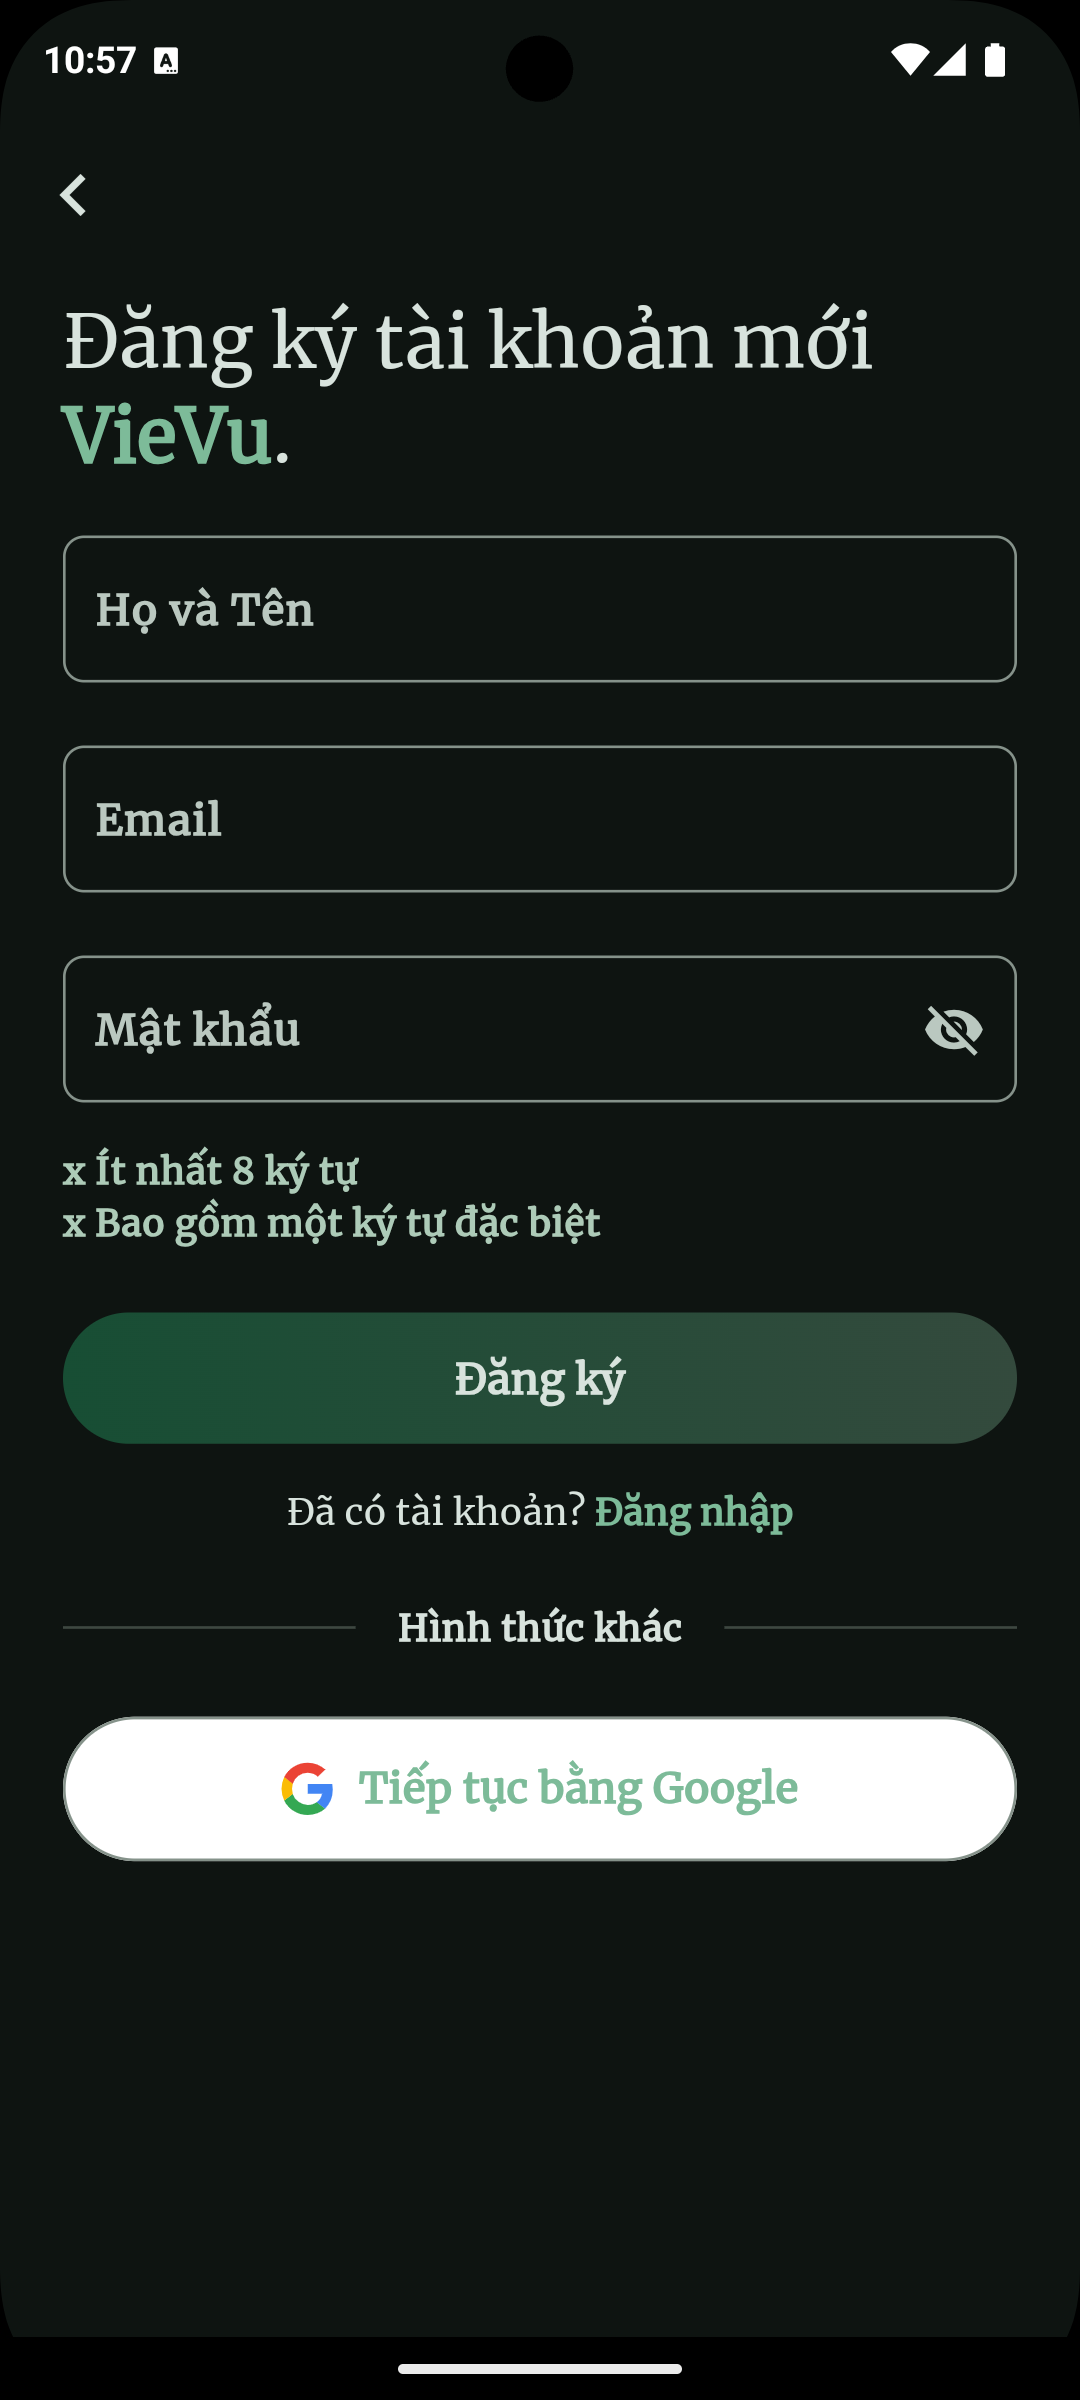
\includegraphics[width=1\linewidth]{figures/c4/system_func/sign_up.png}
        \caption{Form đăng ký}
        \label{fig:func_sign_up}
    \end{subfigure}
    \hfill
    \begin{subfigure}{0.326\textwidth}
        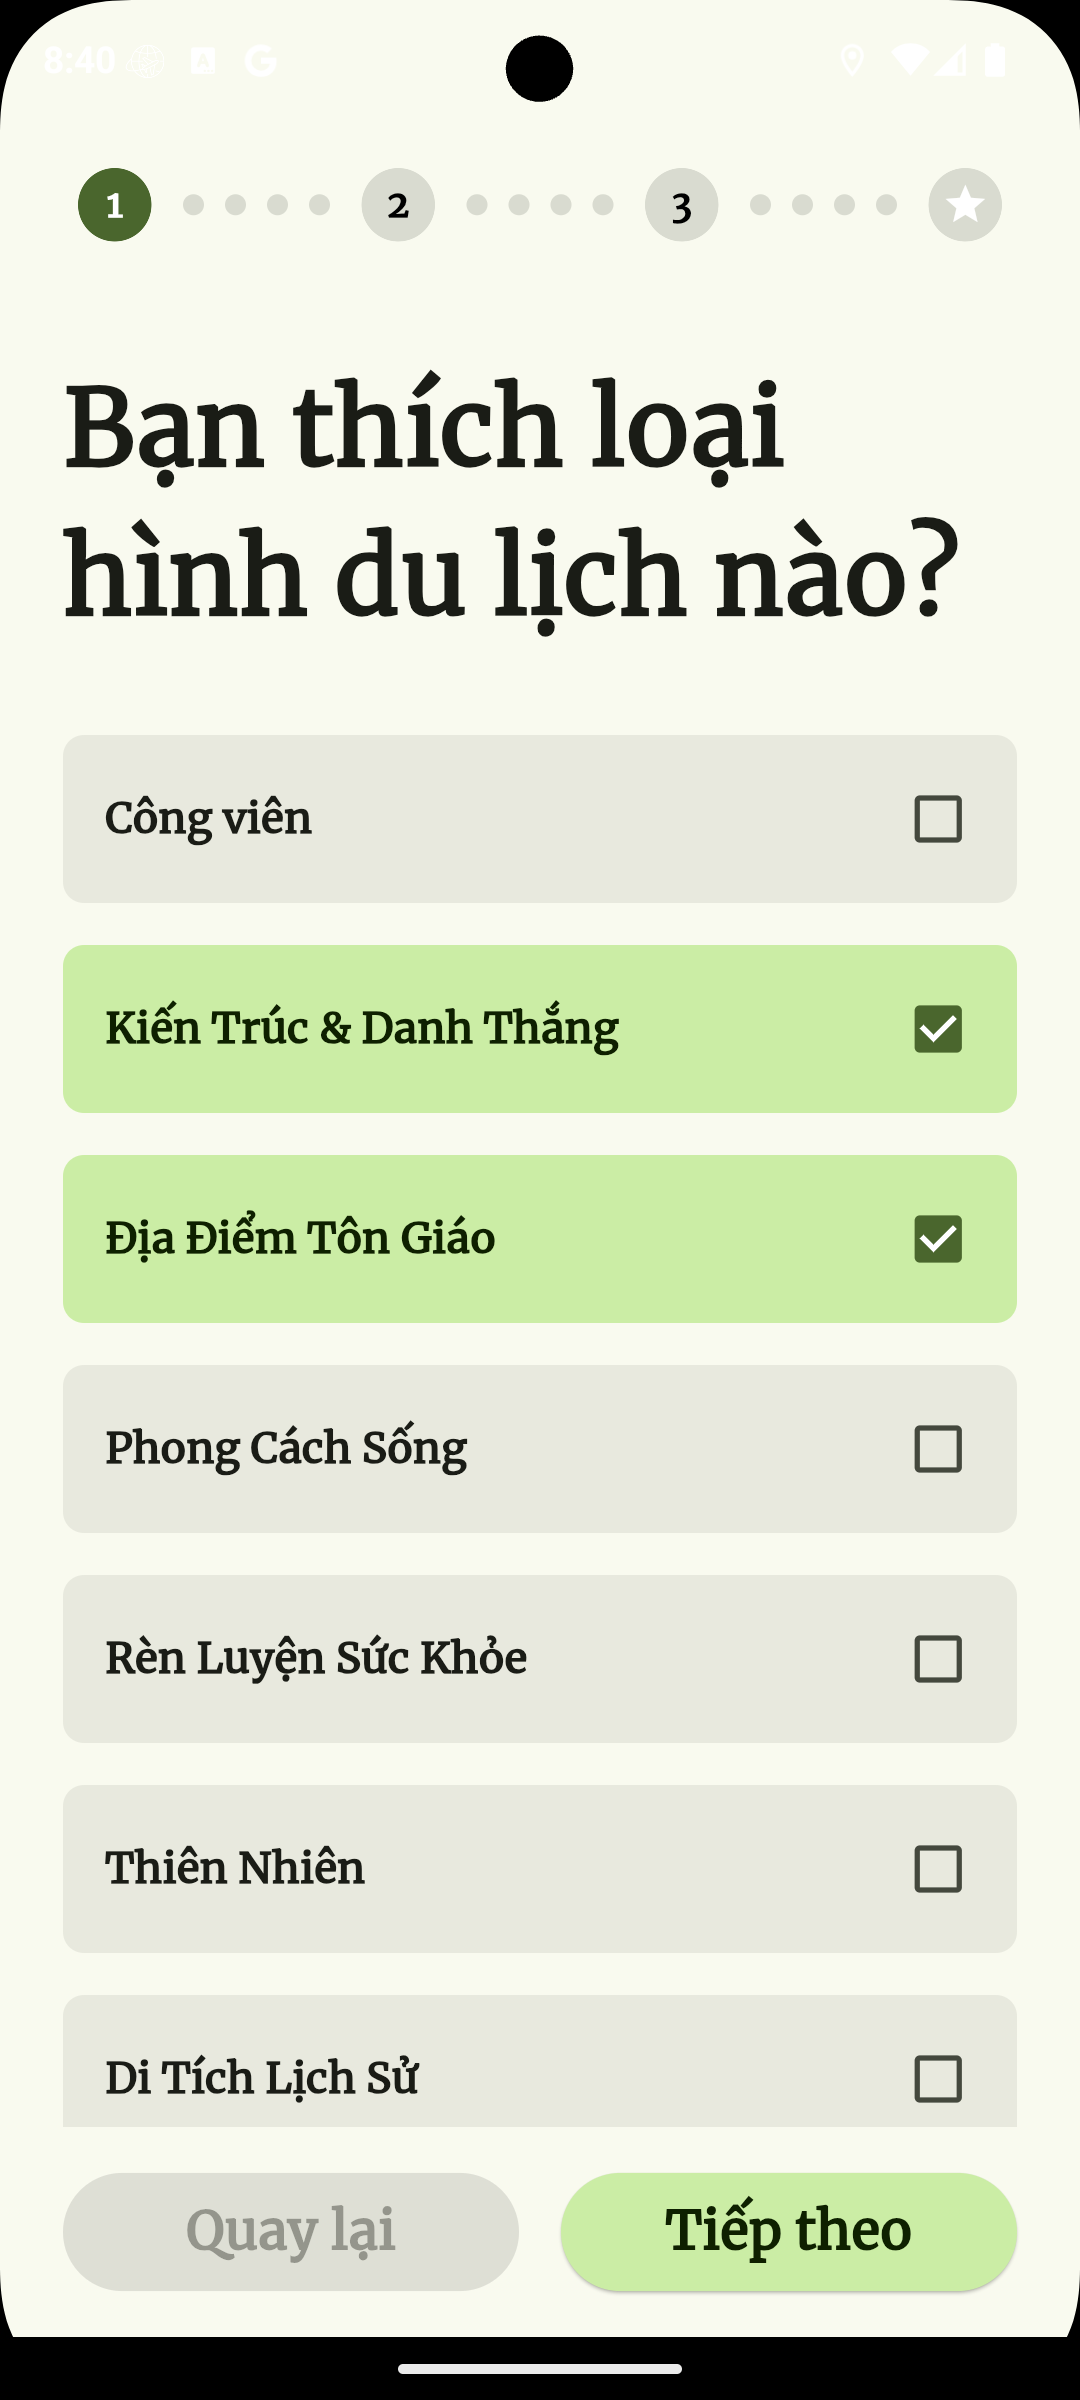
\includegraphics[width=1\linewidth]{figures/c4/system_func/pref.png}
        \caption{Khảo sát sở thích}
        \label{fig:func_pref}
    \end{subfigure}
    \hfill
    \begin{subfigure}{0.326\textwidth}
        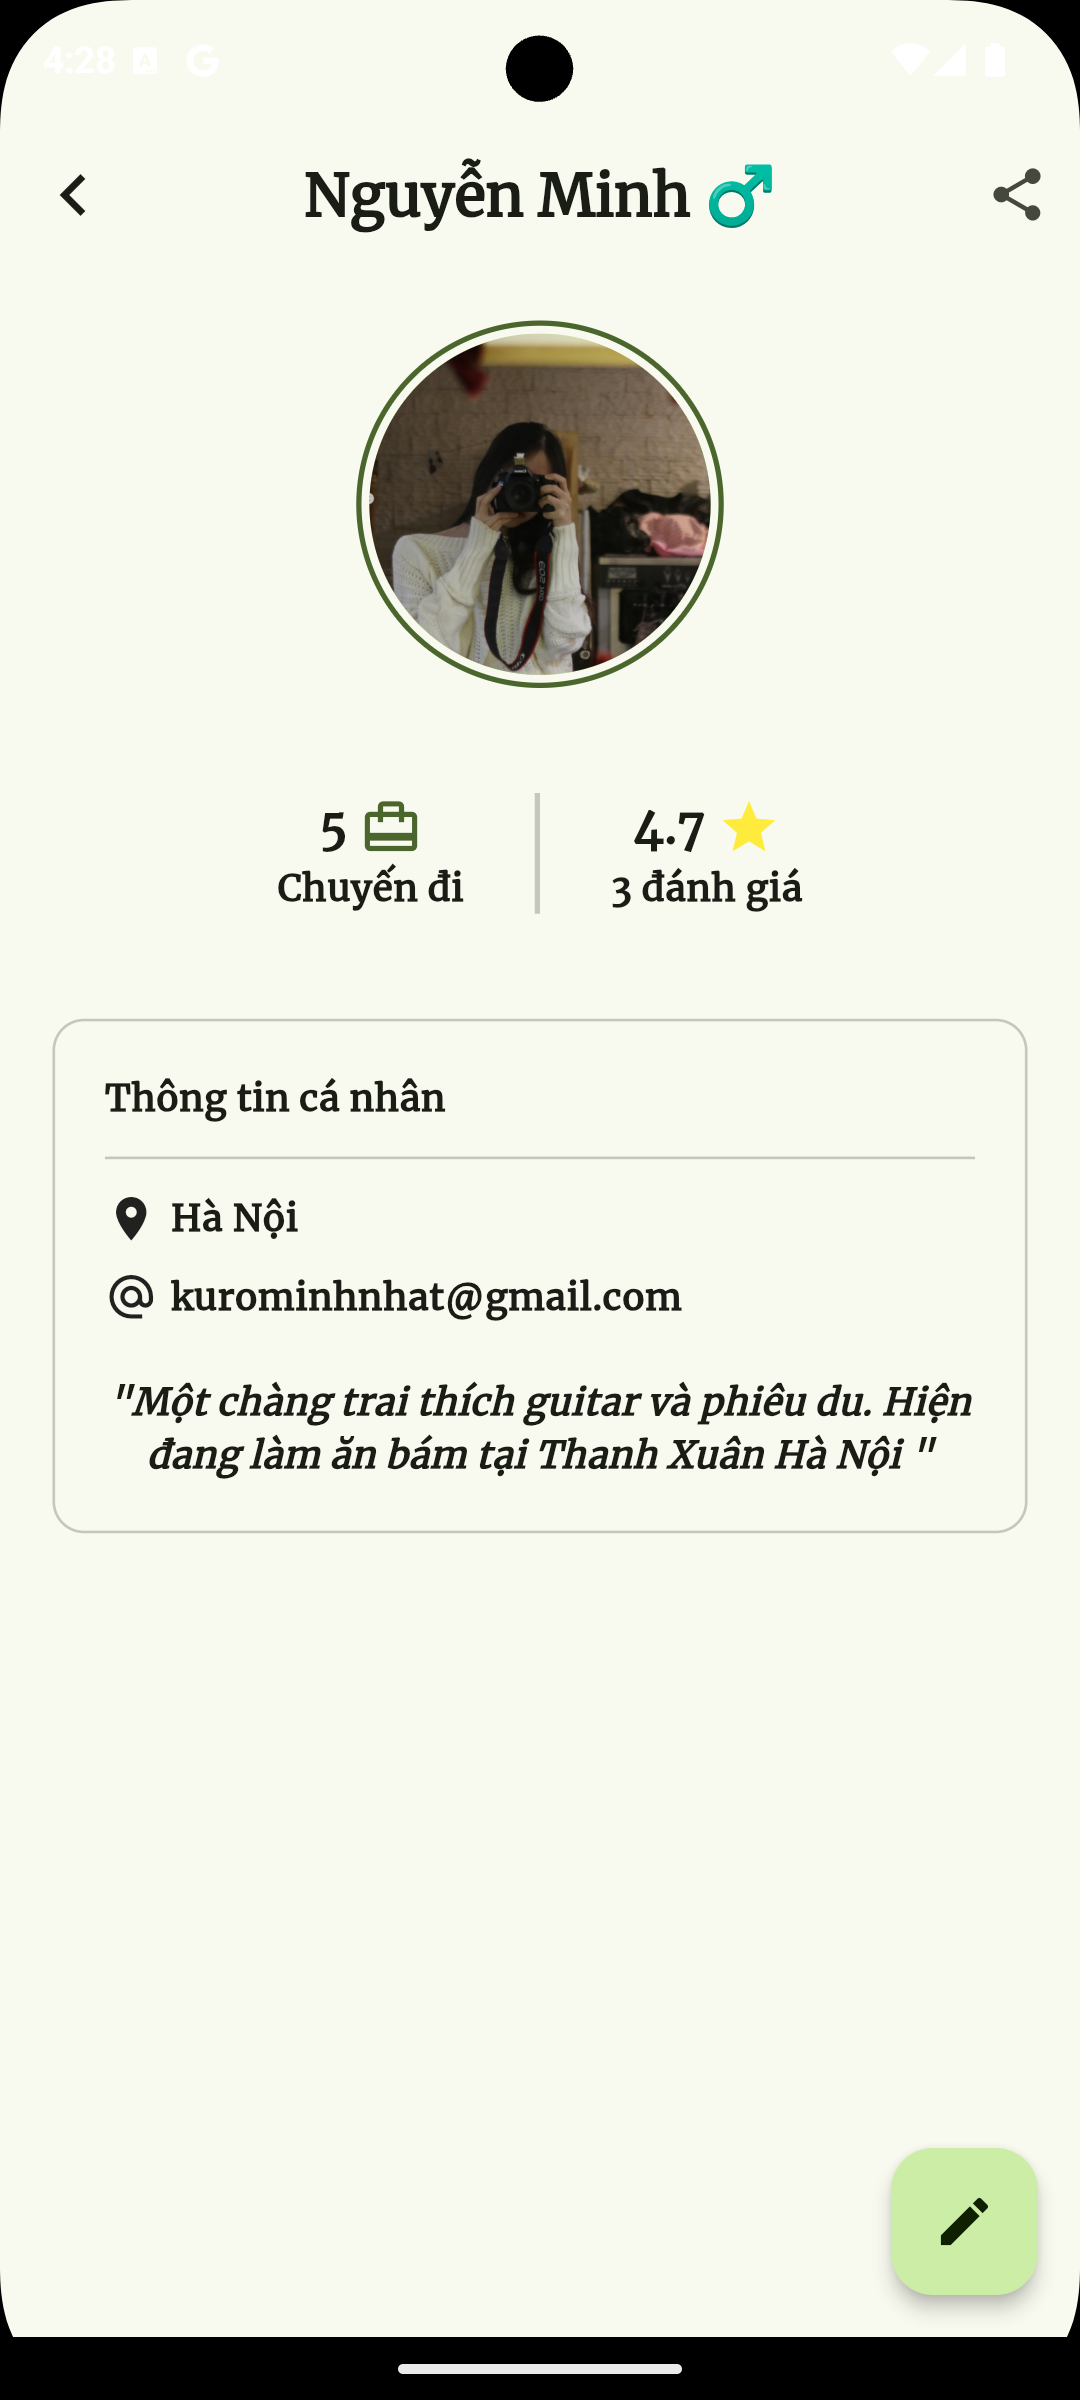
\includegraphics[width=1\linewidth]{figures/c4/system_func/profile.png}
        \caption{Hồ sơ cá nhân}
        \label{fig:func_profile}
    \end{subfigure}
    \caption{Giao diện xác thực và hồ sơ người dùng.}
    \label{fig:auth-screen}
\end{figure}

\subsection{Trang chủ và Giới thiệu}
\noindent Sau khi xác thực, người dùng được dẫn đến màn hình giới thiệu ngắn gọn (Hình~\ref{fig:func_intro}) trước khi vào trang chính của ứng dụng. Trang chủ (Hình~\ref{fig:func_home}) là nơi hiển thị danh sách các chuyến đi công khai mà người dùng có thể tham gia. Chức năng tìm kiếm (Hình~\ref{fig:func_search_home}) cho phép lọc các chuyến đi theo từ khóa. Các giao diện này được minh họa trong Hình~\ref{fig:home-screen}.

\begin{figure}[H]
    \centering
    \begin{subfigure}{0.326\textwidth}
        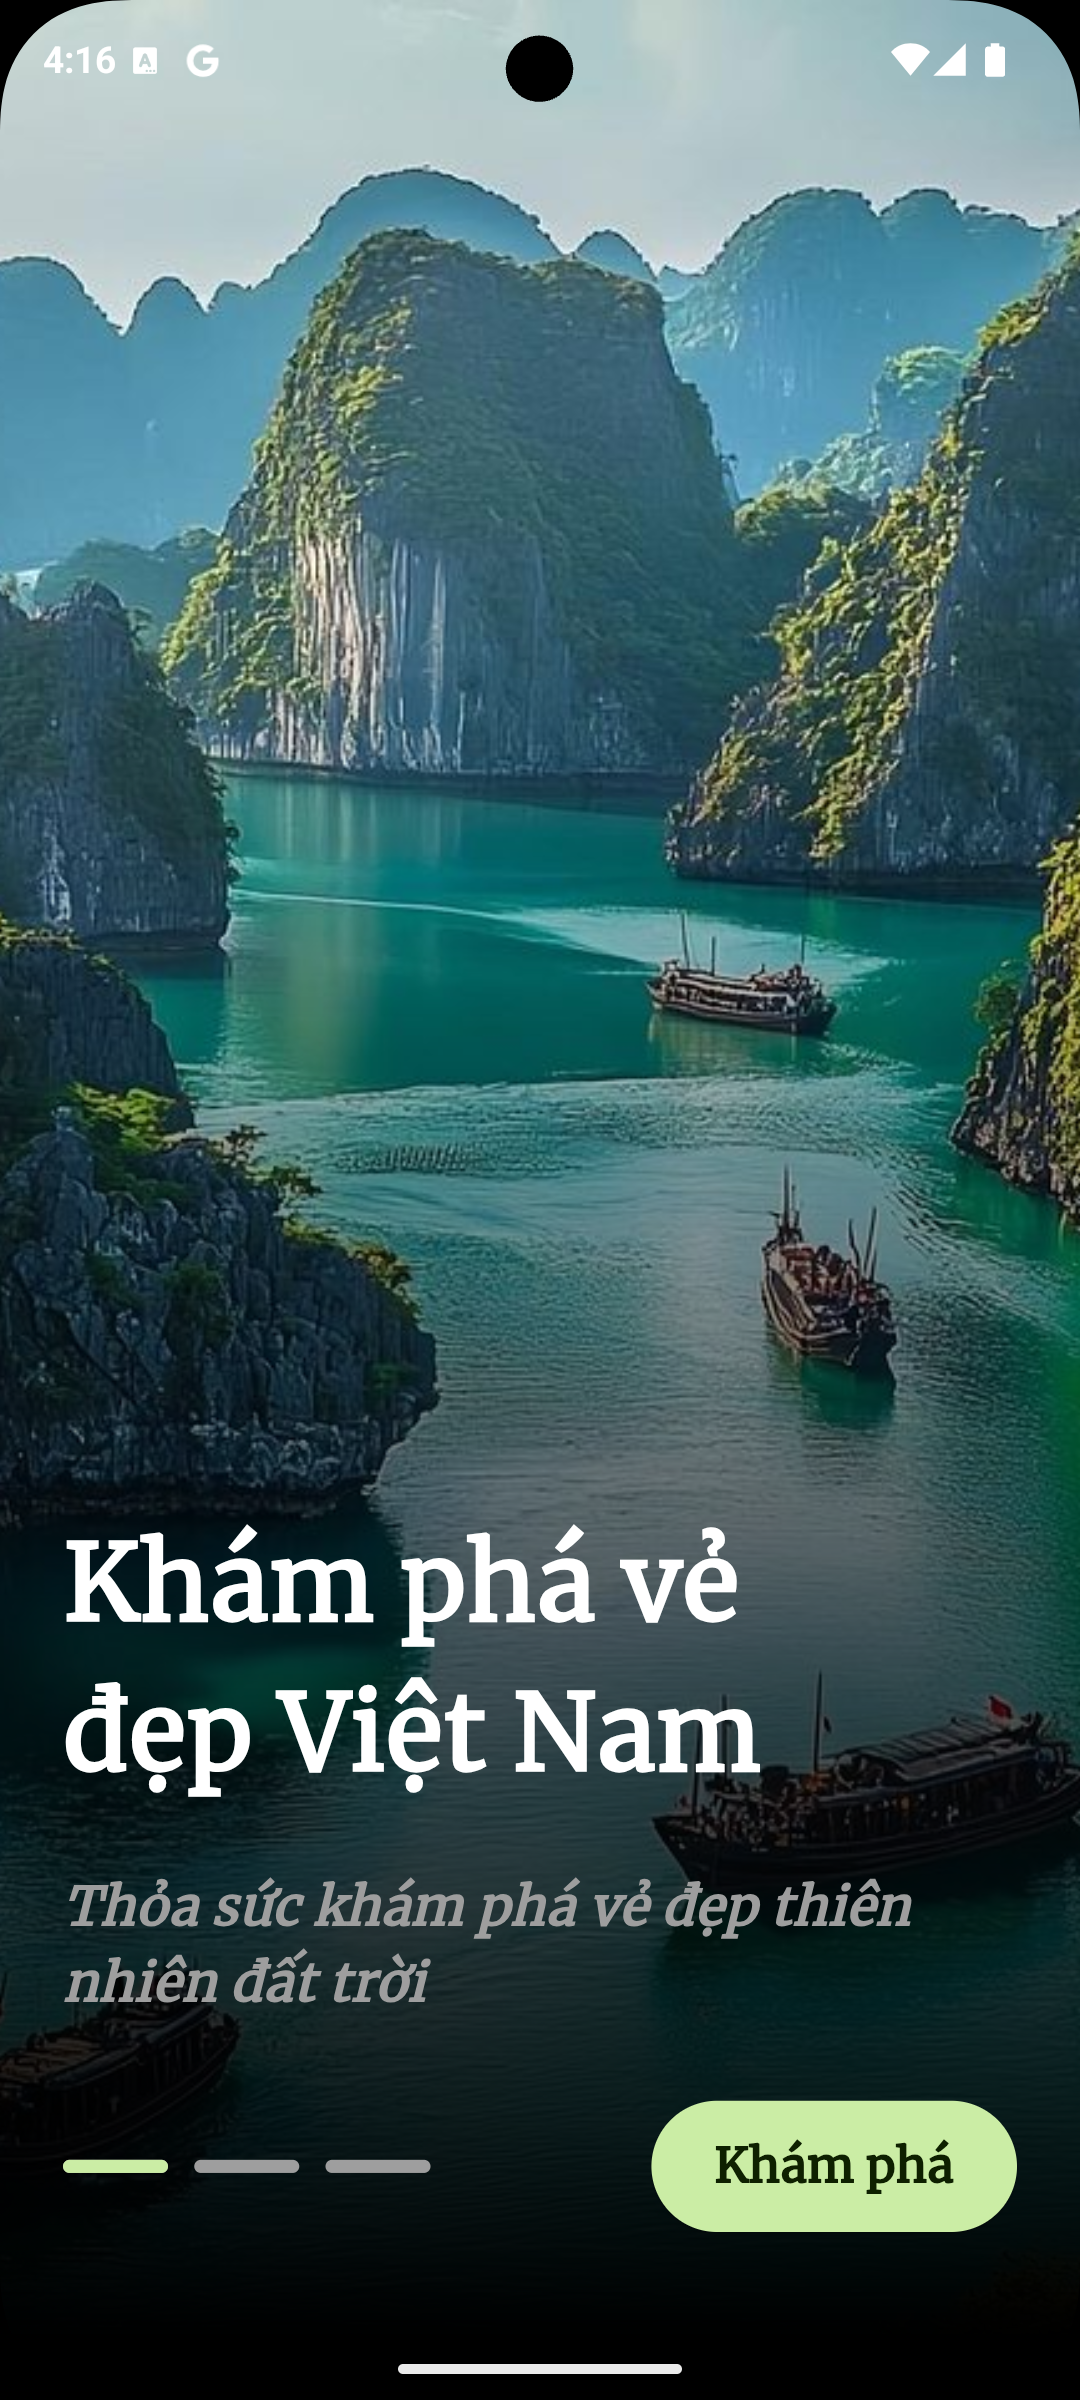
\includegraphics[width=1\linewidth]{figures/c4/system_func/intro.png}
        \caption{Màn hình giới thiệu}
        \label{fig:func_intro}
    \end{subfigure}
    \hfill
    \begin{subfigure}{0.326\textwidth}
        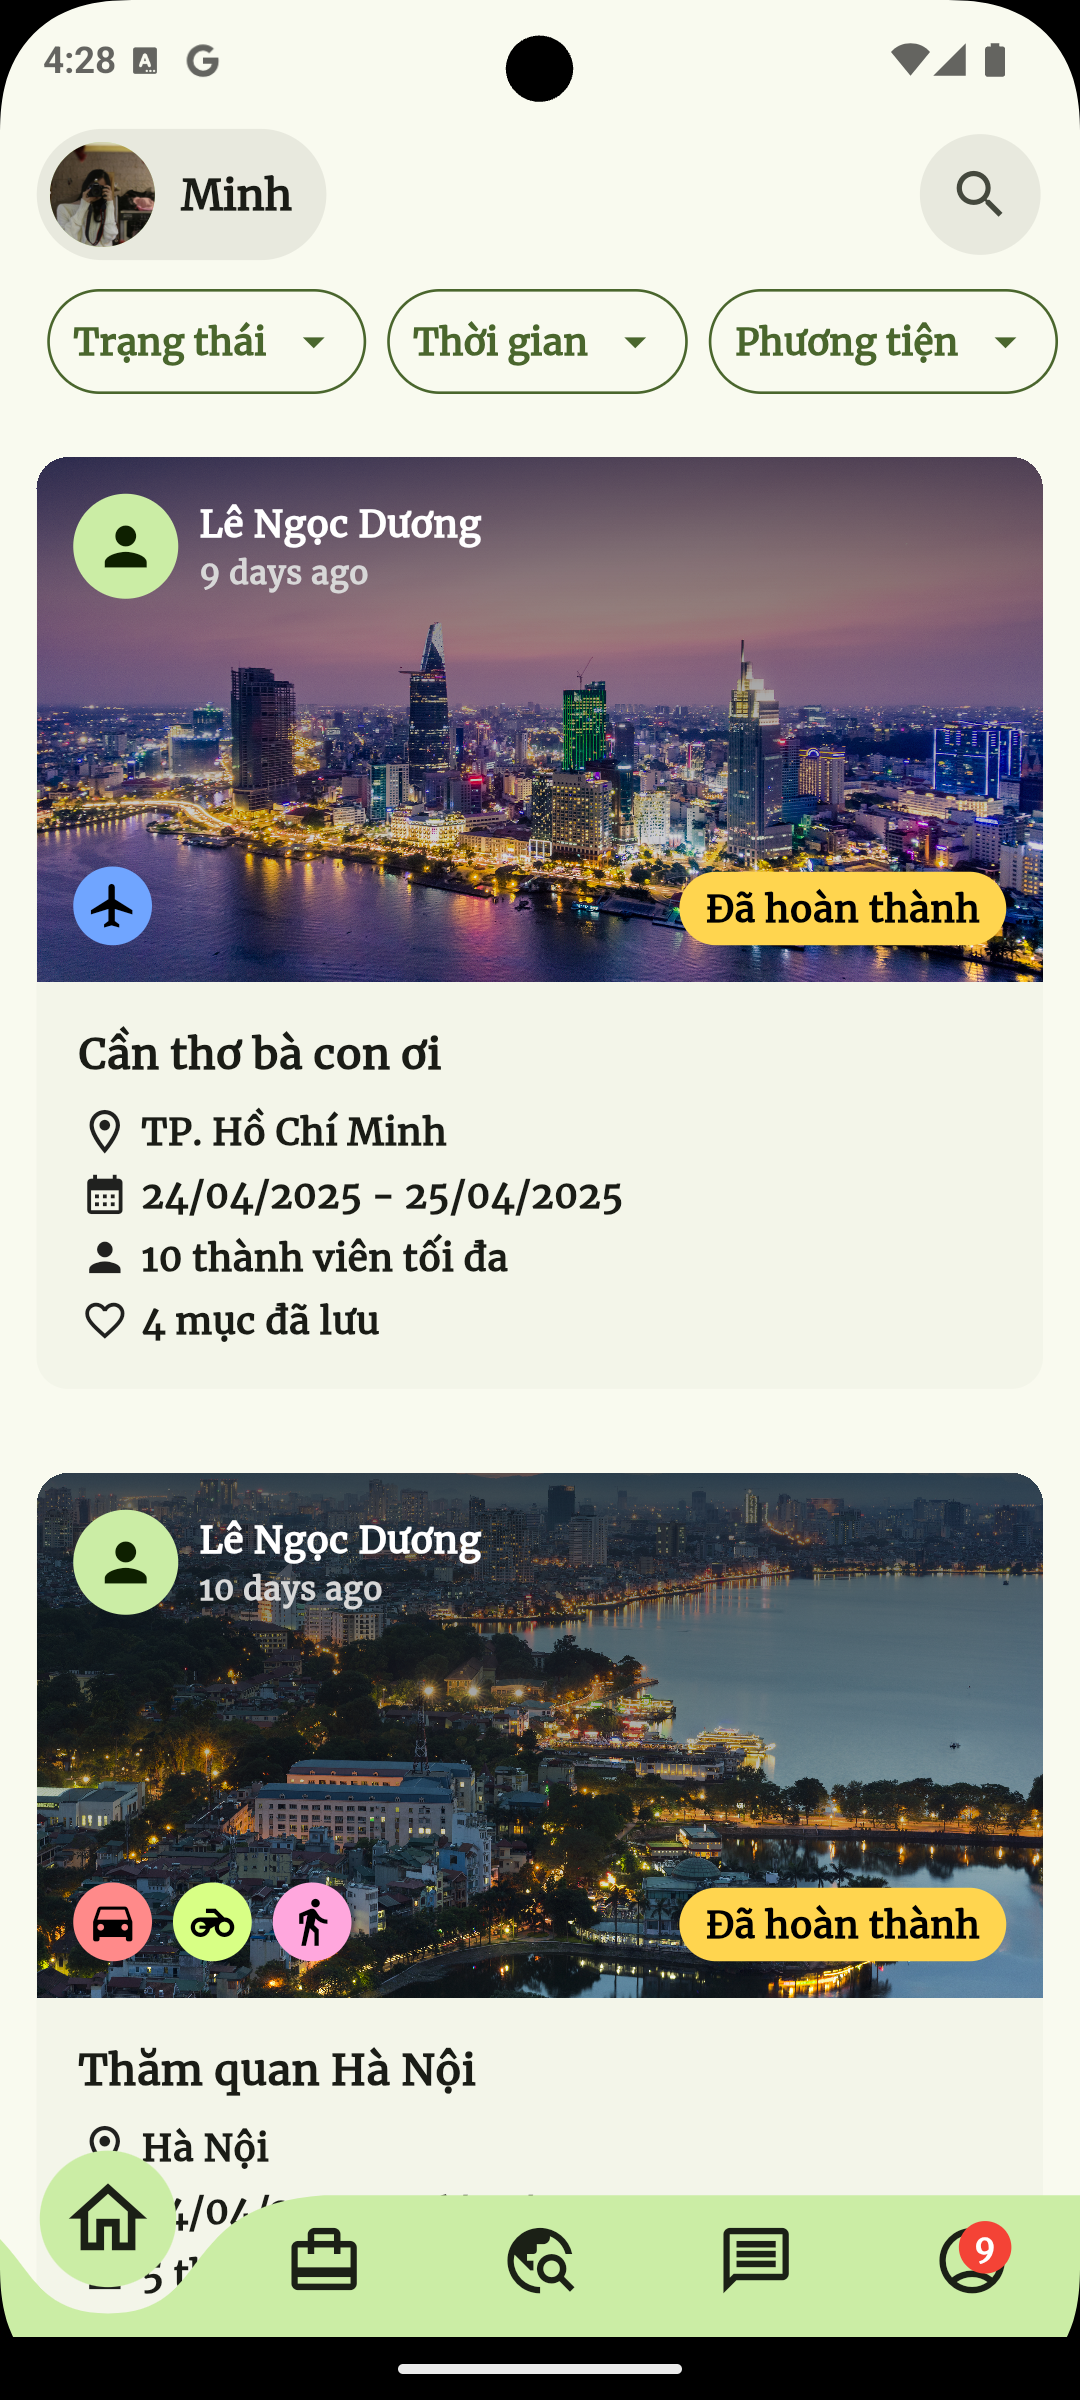
\includegraphics[width=1\linewidth]{figures/c4/system_func/home.png}
        \caption{Trang chủ}
        \label{fig:func_home}
    \end{subfigure}
    \hfill
    \begin{subfigure}{0.326\textwidth}
        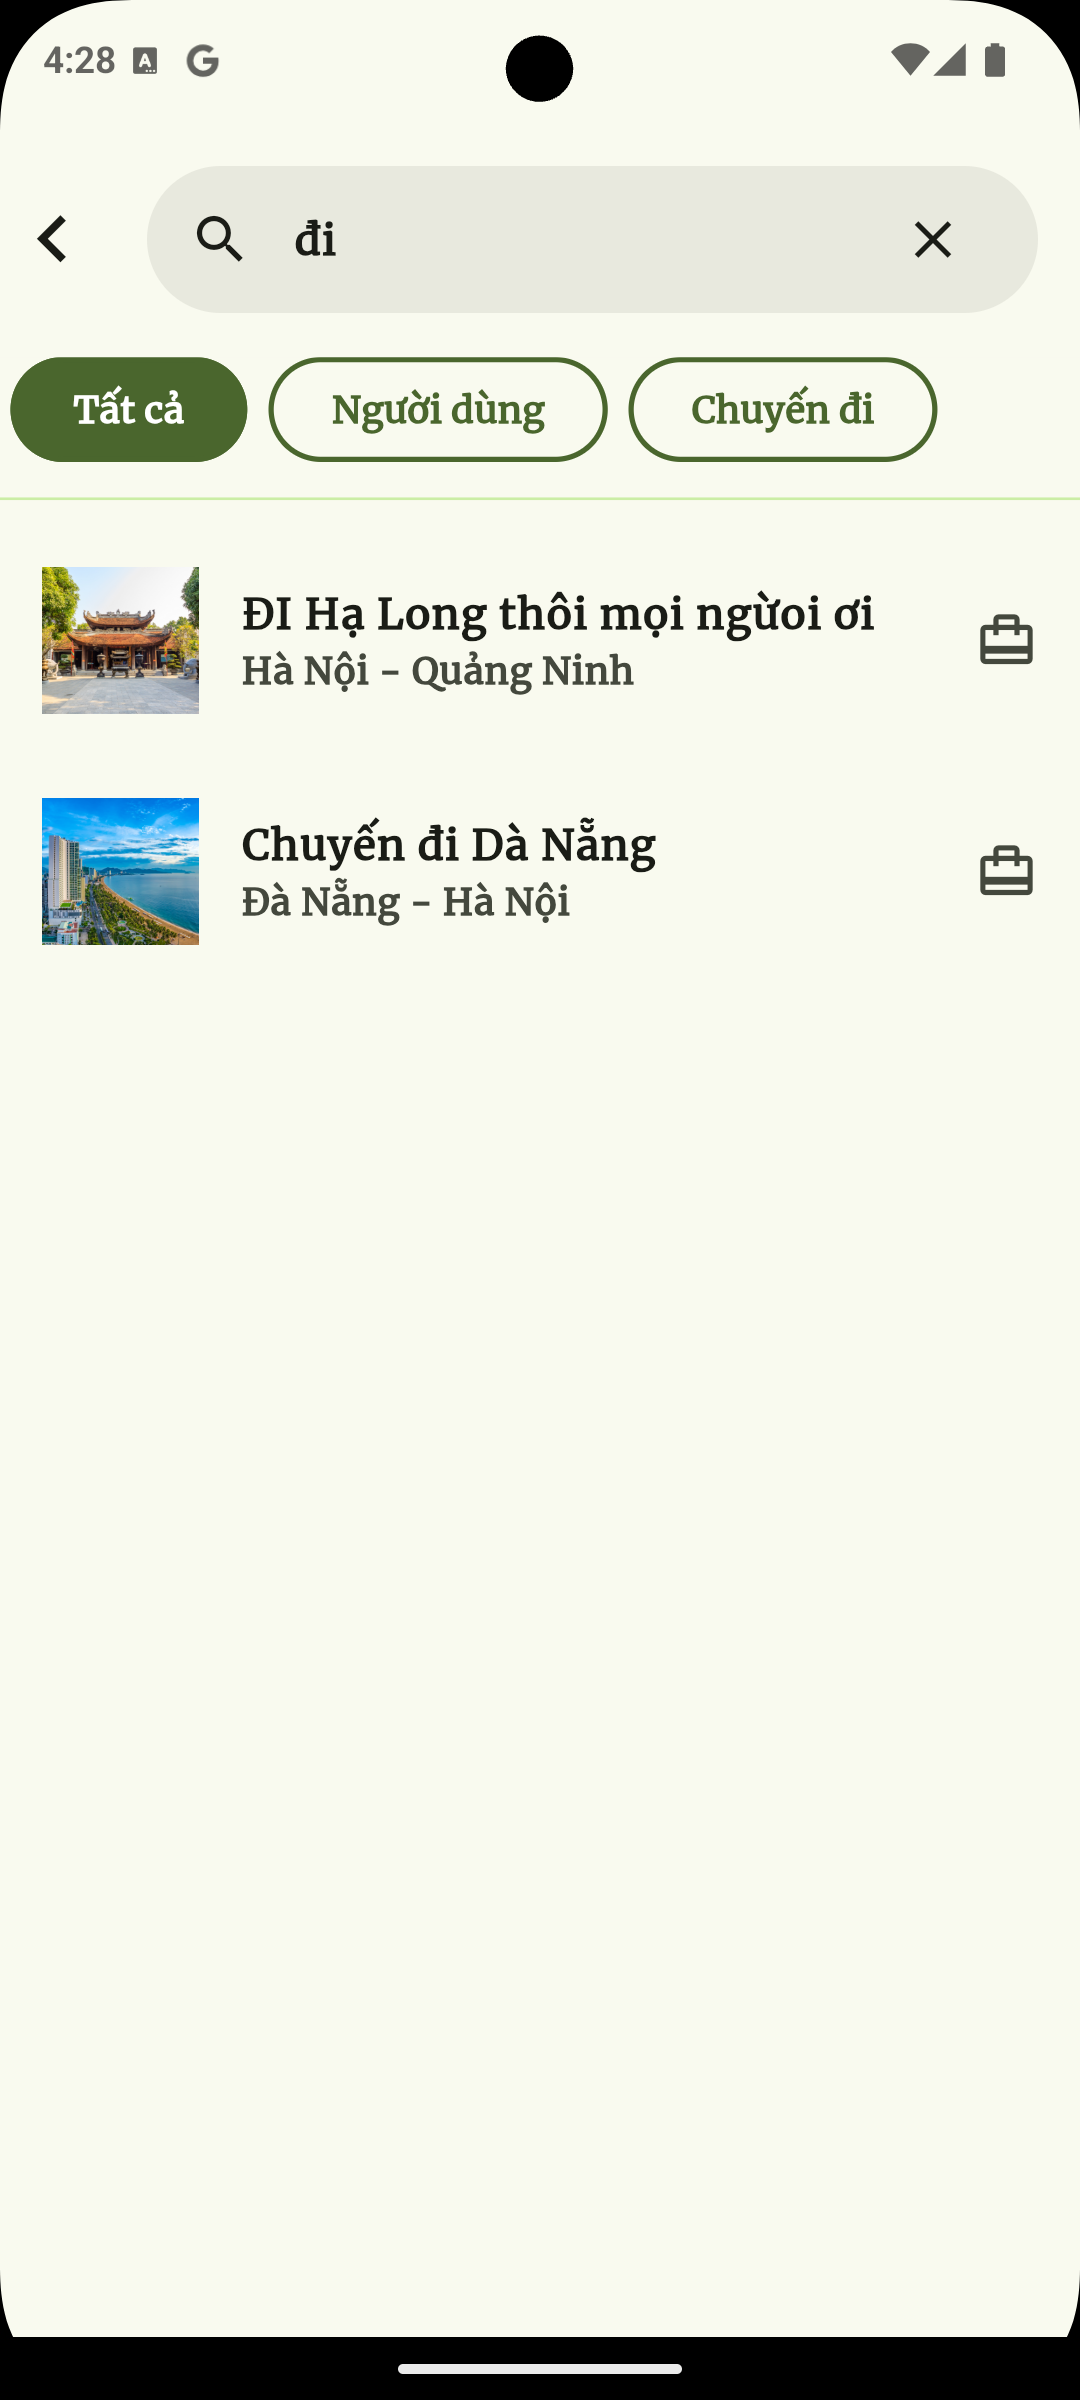
\includegraphics[width=1\linewidth]{figures/c4/system_func/search_home.png}
        \caption{Tìm kiếm chuyến đi}
        \label{fig:func_search_home}
    \end{subfigure}
    \caption{Giao diện giới thiệu và trang chủ.}
    \label{fig:home-screen}
\end{figure}

\subsection{Khám phá Thông tin Du lịch}
\noindent Người dùng có thể xem danh sách các địa điểm, sự kiện (Hình~\ref{fig:func_explore}), xem thông tin chi tiết và đánh giá của một địa điểm cụ thể (Hình~\ref{fig:func_att_detail}), hoặc trực quan hóa vị trí các địa điểm trên bản đồ (Hình~\ref{fig:func_map_loc}). Hệ thống cũng hỗ trợ tìm kiếm các dịch vụ lân cận vị trí hiện tại (Hình~\ref{fig:func_nearby}), tìm kiếm theo từ khóa (Hình~\ref{fig:func_search_loc}), và lọc kết quả theo tiêu chí như loại hình, giá, đánh giá (ví dụ lọc nhà hàng Hình~\ref{fig:func_filter_res}).

\begin{figure}[H]
    \centering
    % --- First Row ---
    \begin{subfigure}{0.326\textwidth}
        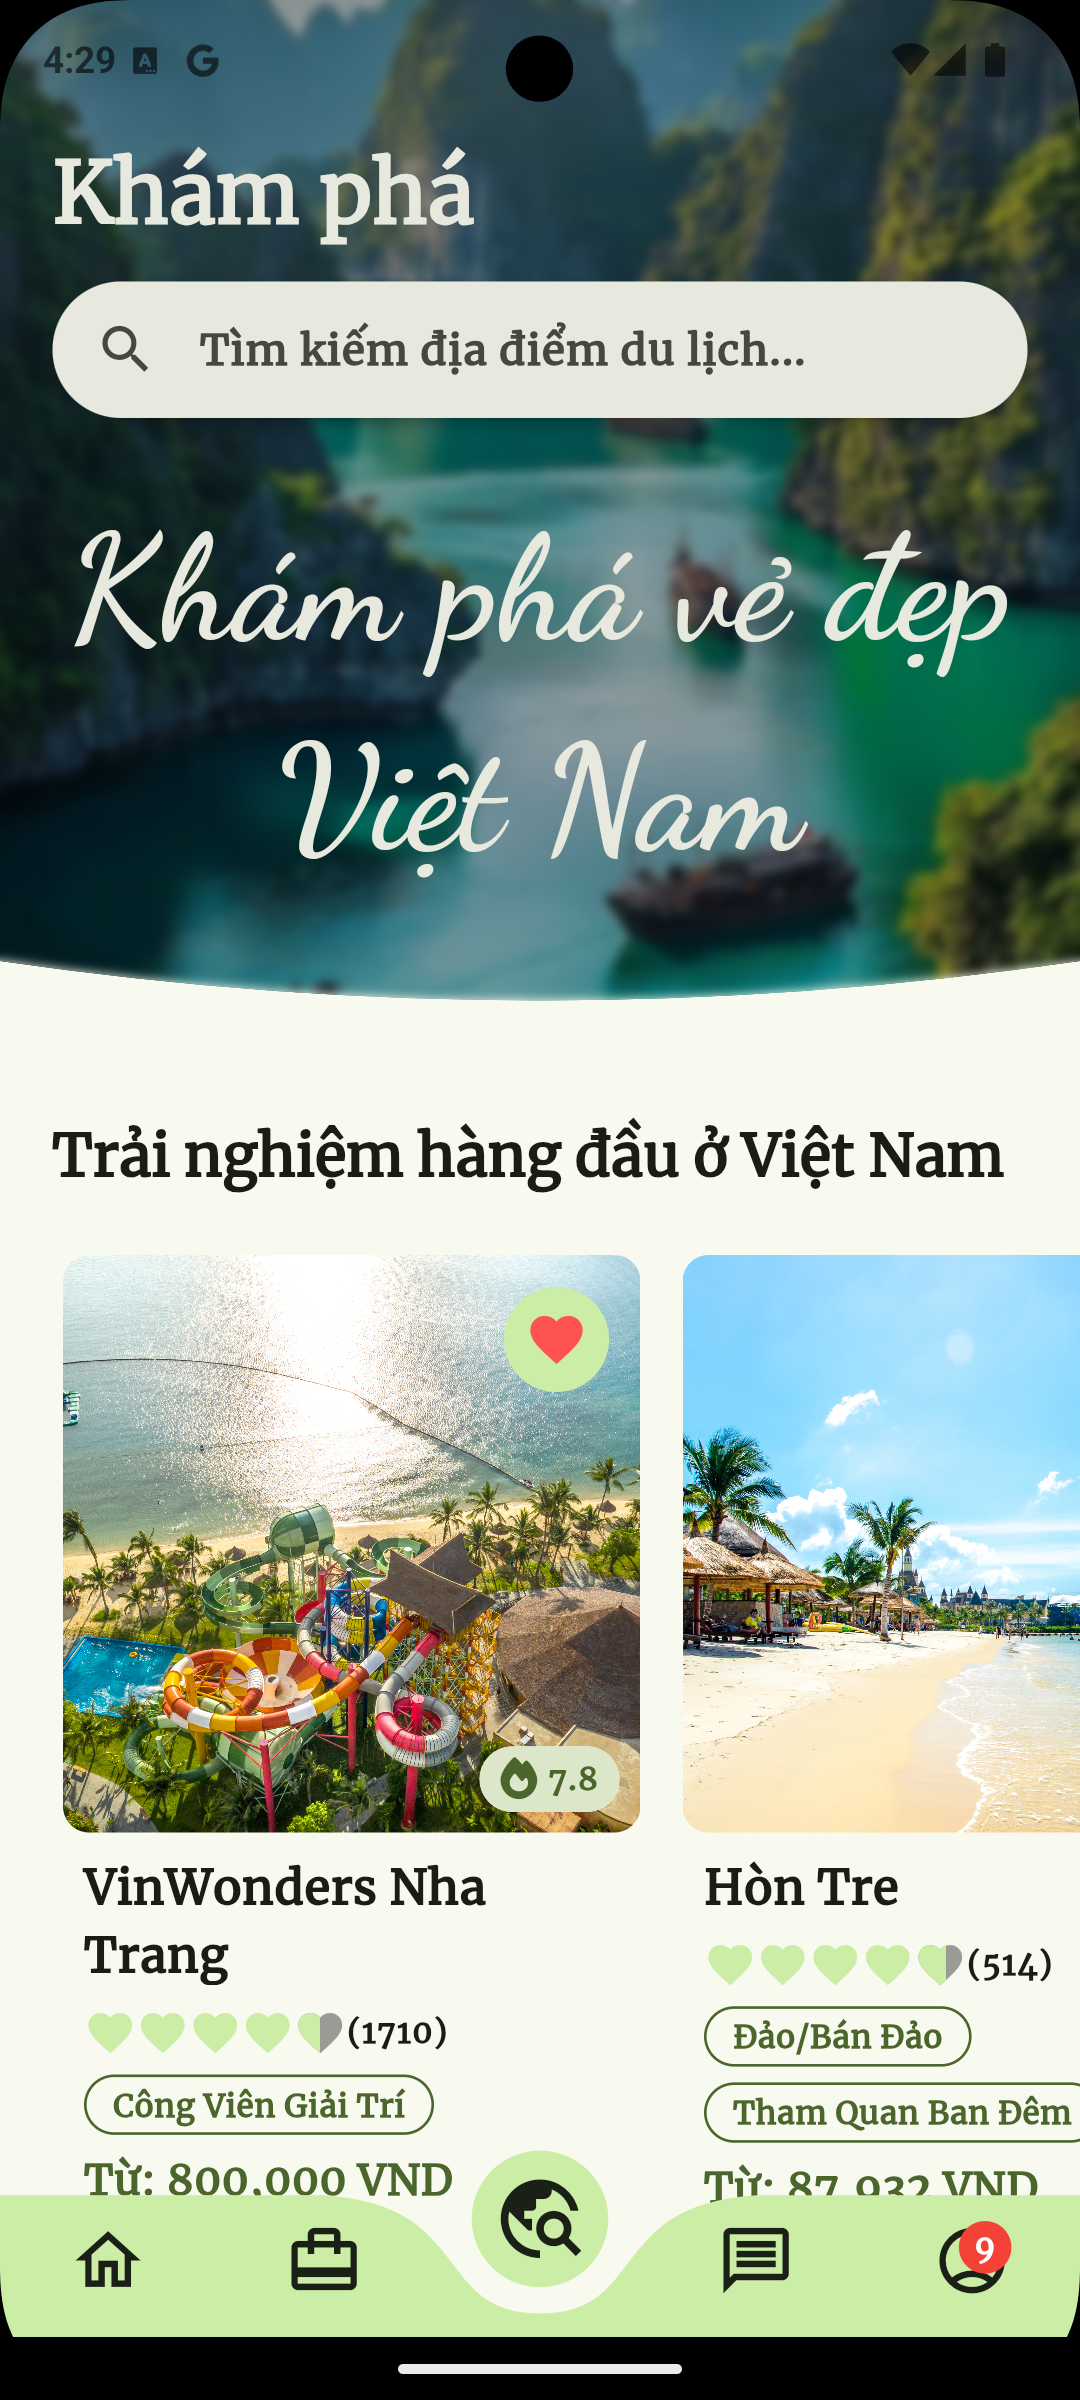
\includegraphics[height=10cm,width=1\linewidth]{figures/c4/system_func/explore.png}
        \caption{Trang Khám phá}
        \label{fig:func_explore}
    \end{subfigure}
    \hfill
    \begin{subfigure}{0.326\textwidth}
        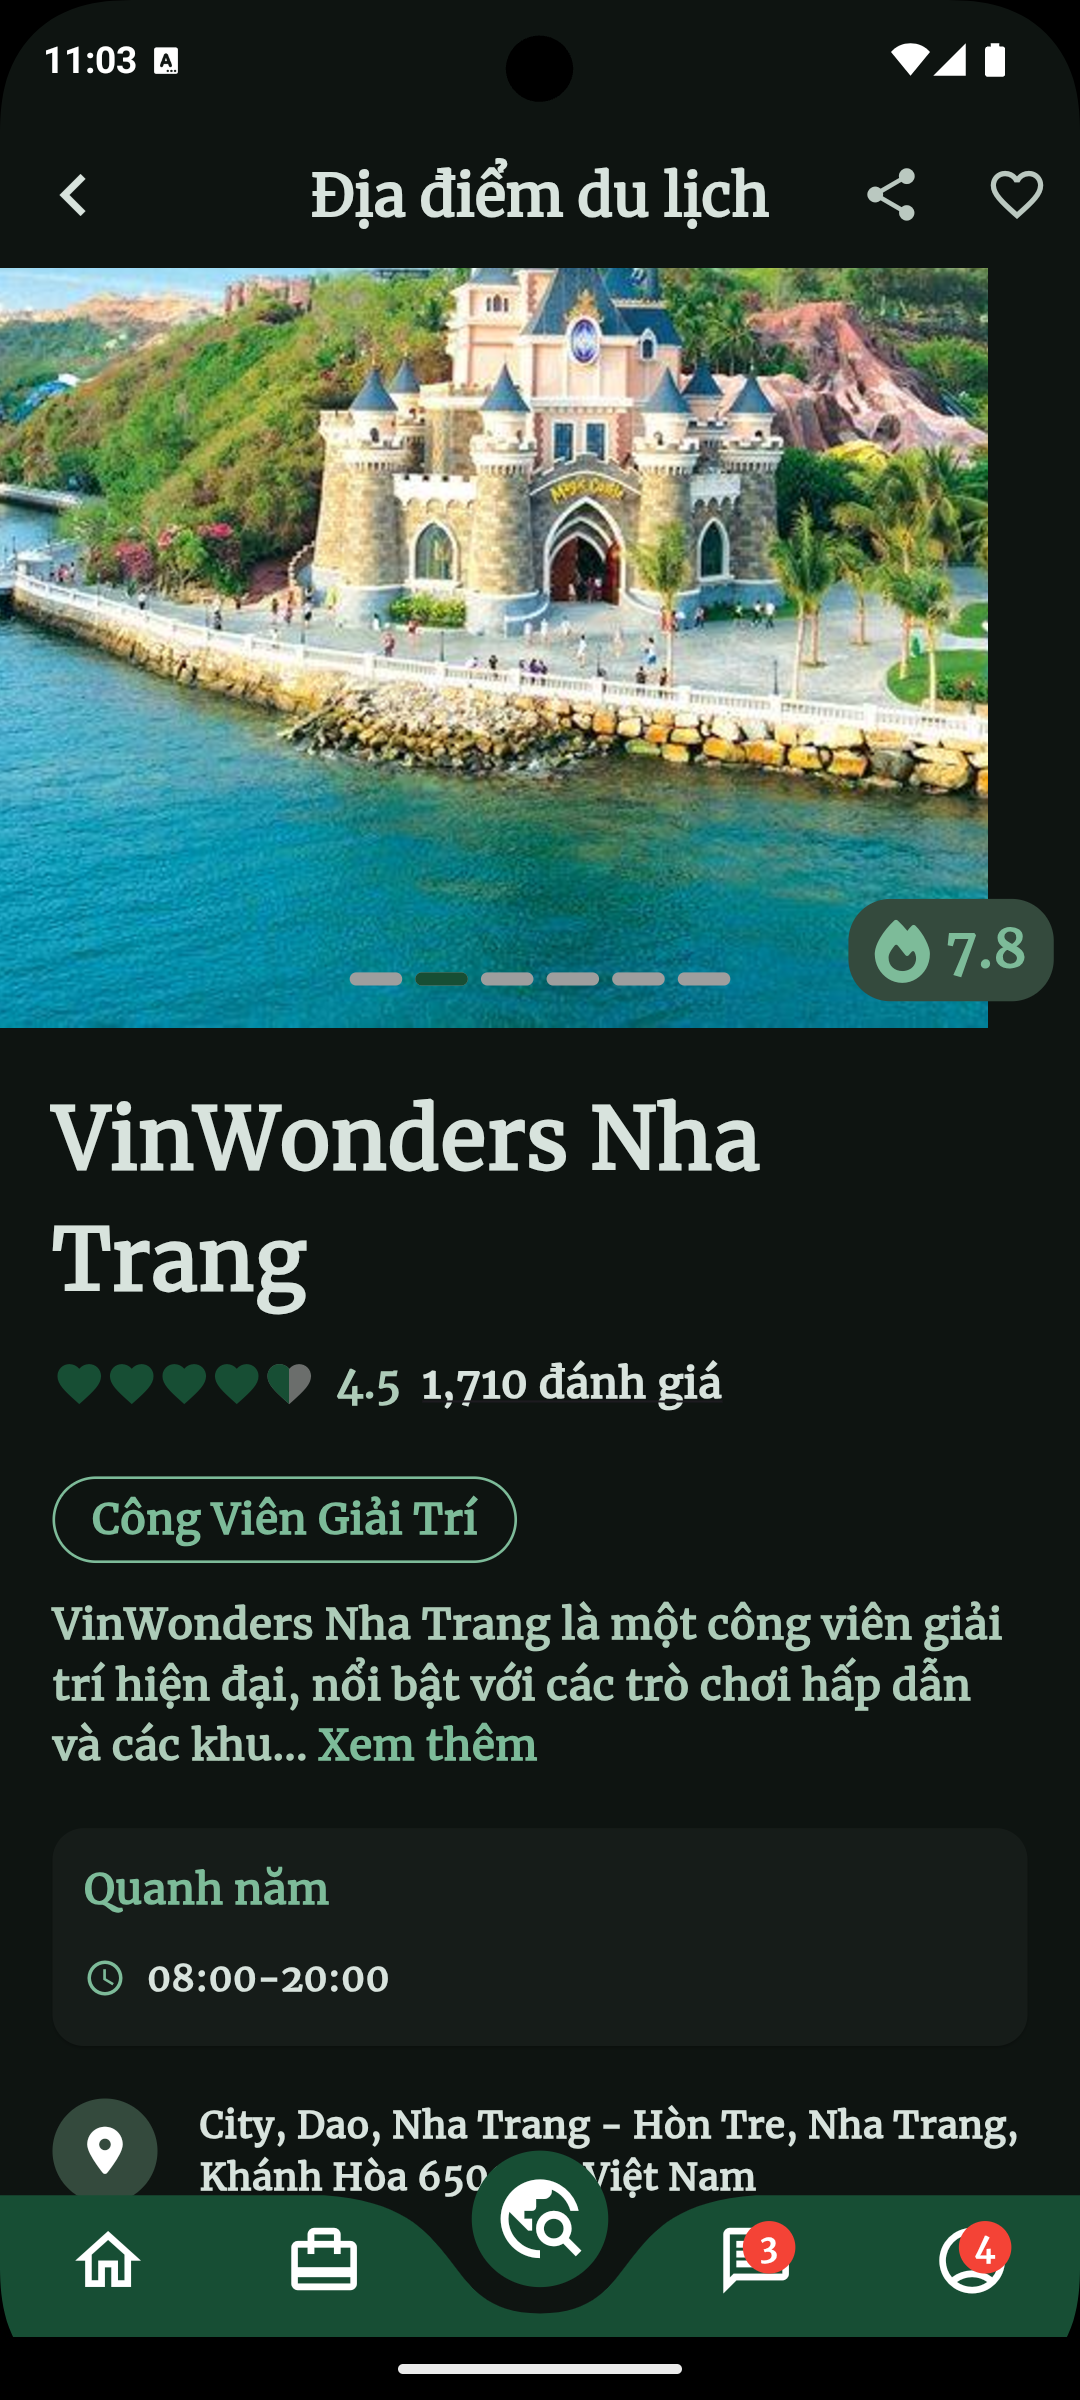
\includegraphics[height=10cm,width=1\linewidth]{figures/c4/system_func/att.png}
        \caption{Chi tiết địa điểm}
        \label{fig:func_att_detail}
    \end{subfigure}
    \hfill
    \begin{subfigure}{0.326\textwidth}
        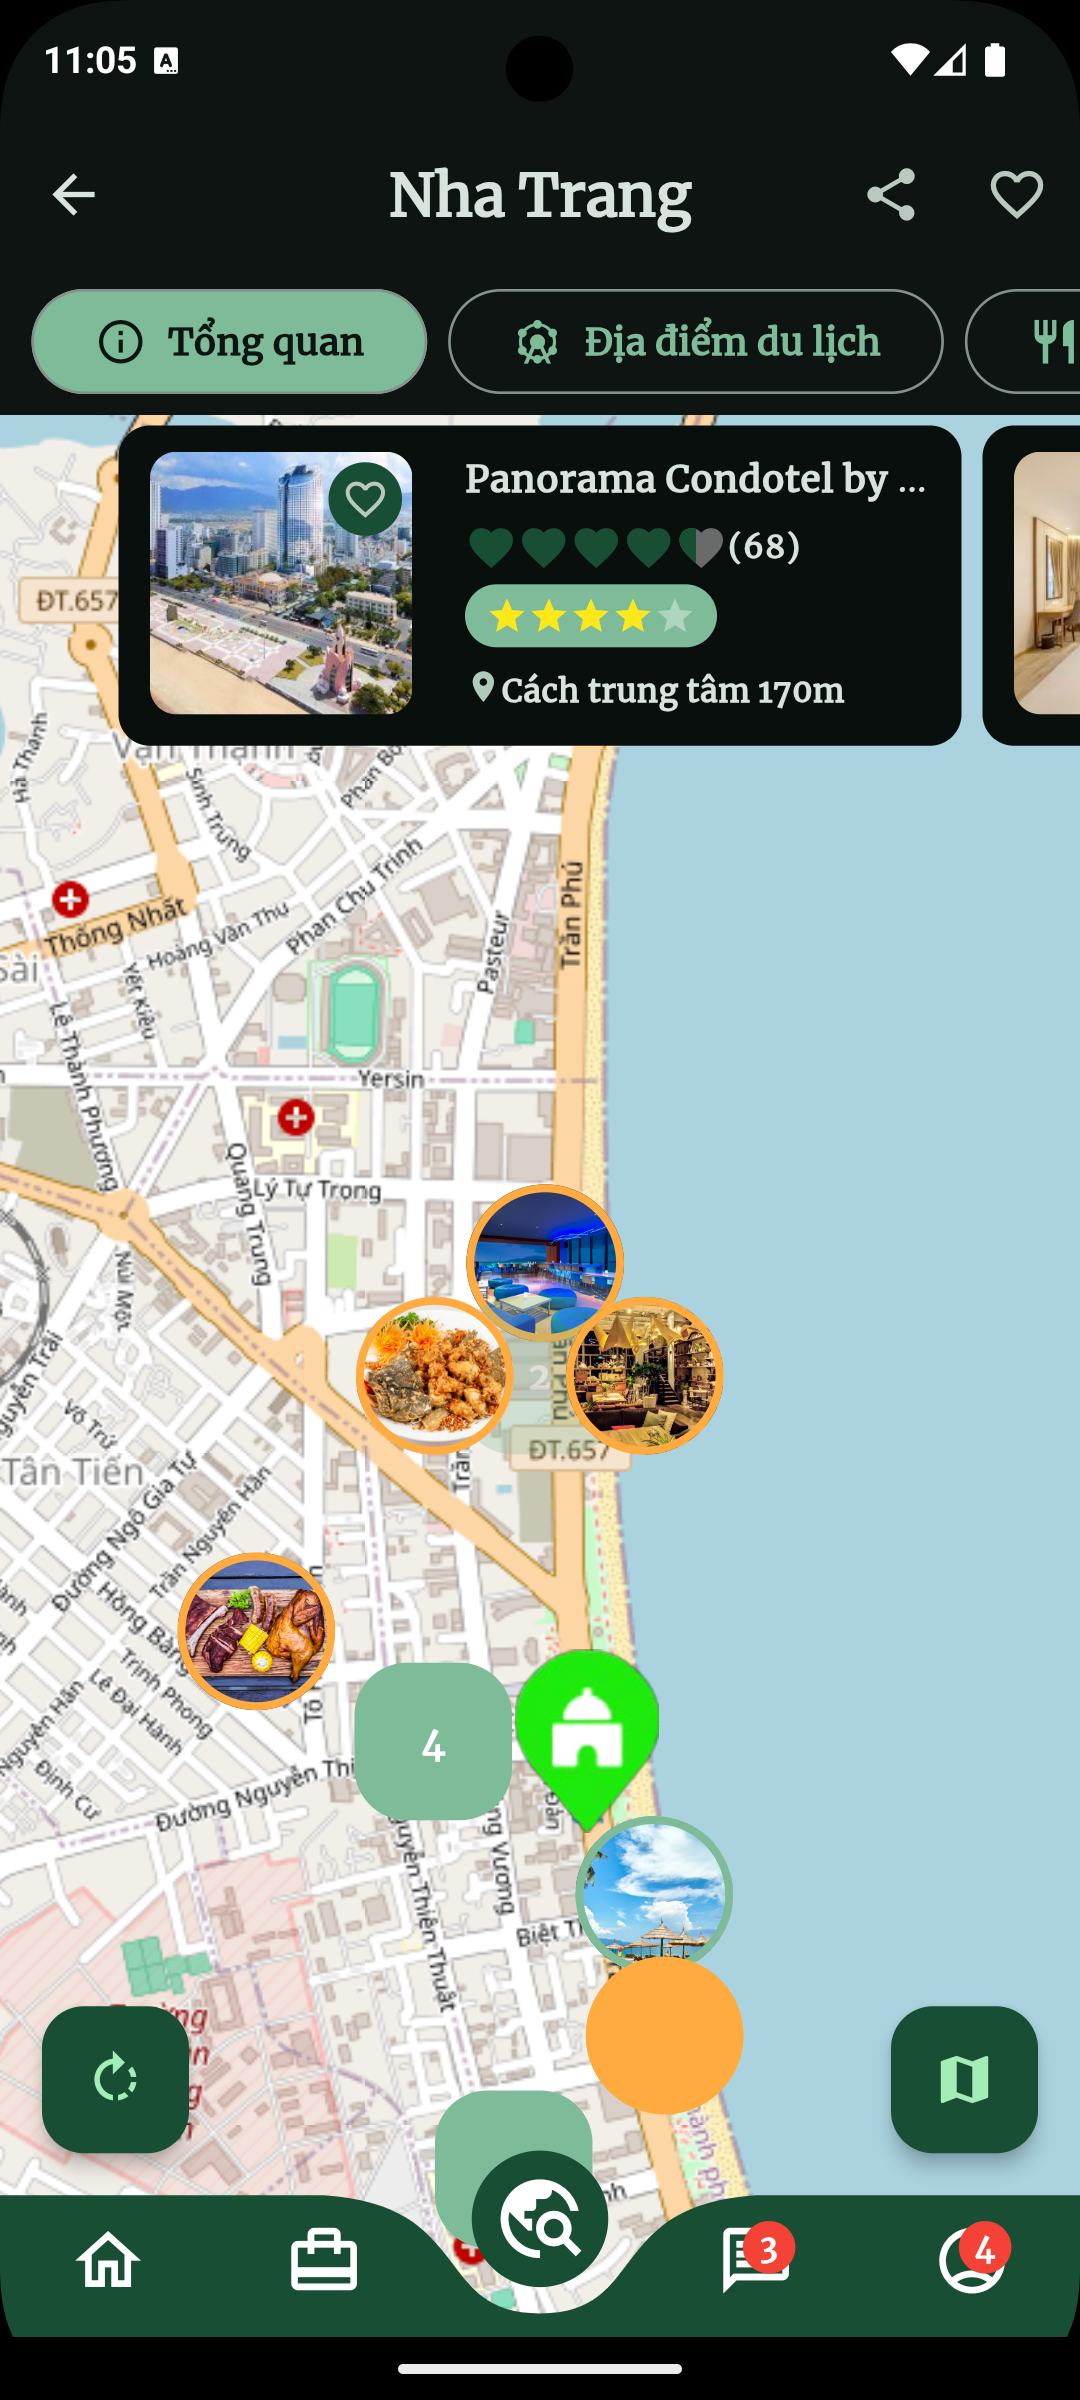
\includegraphics[height=10cm,width=1\linewidth]{figures/c4/system_func/map_loc.png}
        \caption{Xem trên bản đồ}
        \label{fig:func_map_loc}
    \end{subfigure}

    \vspace{\baselineskip} % Vertical space between rows

    % --- Second Row ---
    \begin{subfigure}{0.326\textwidth}
        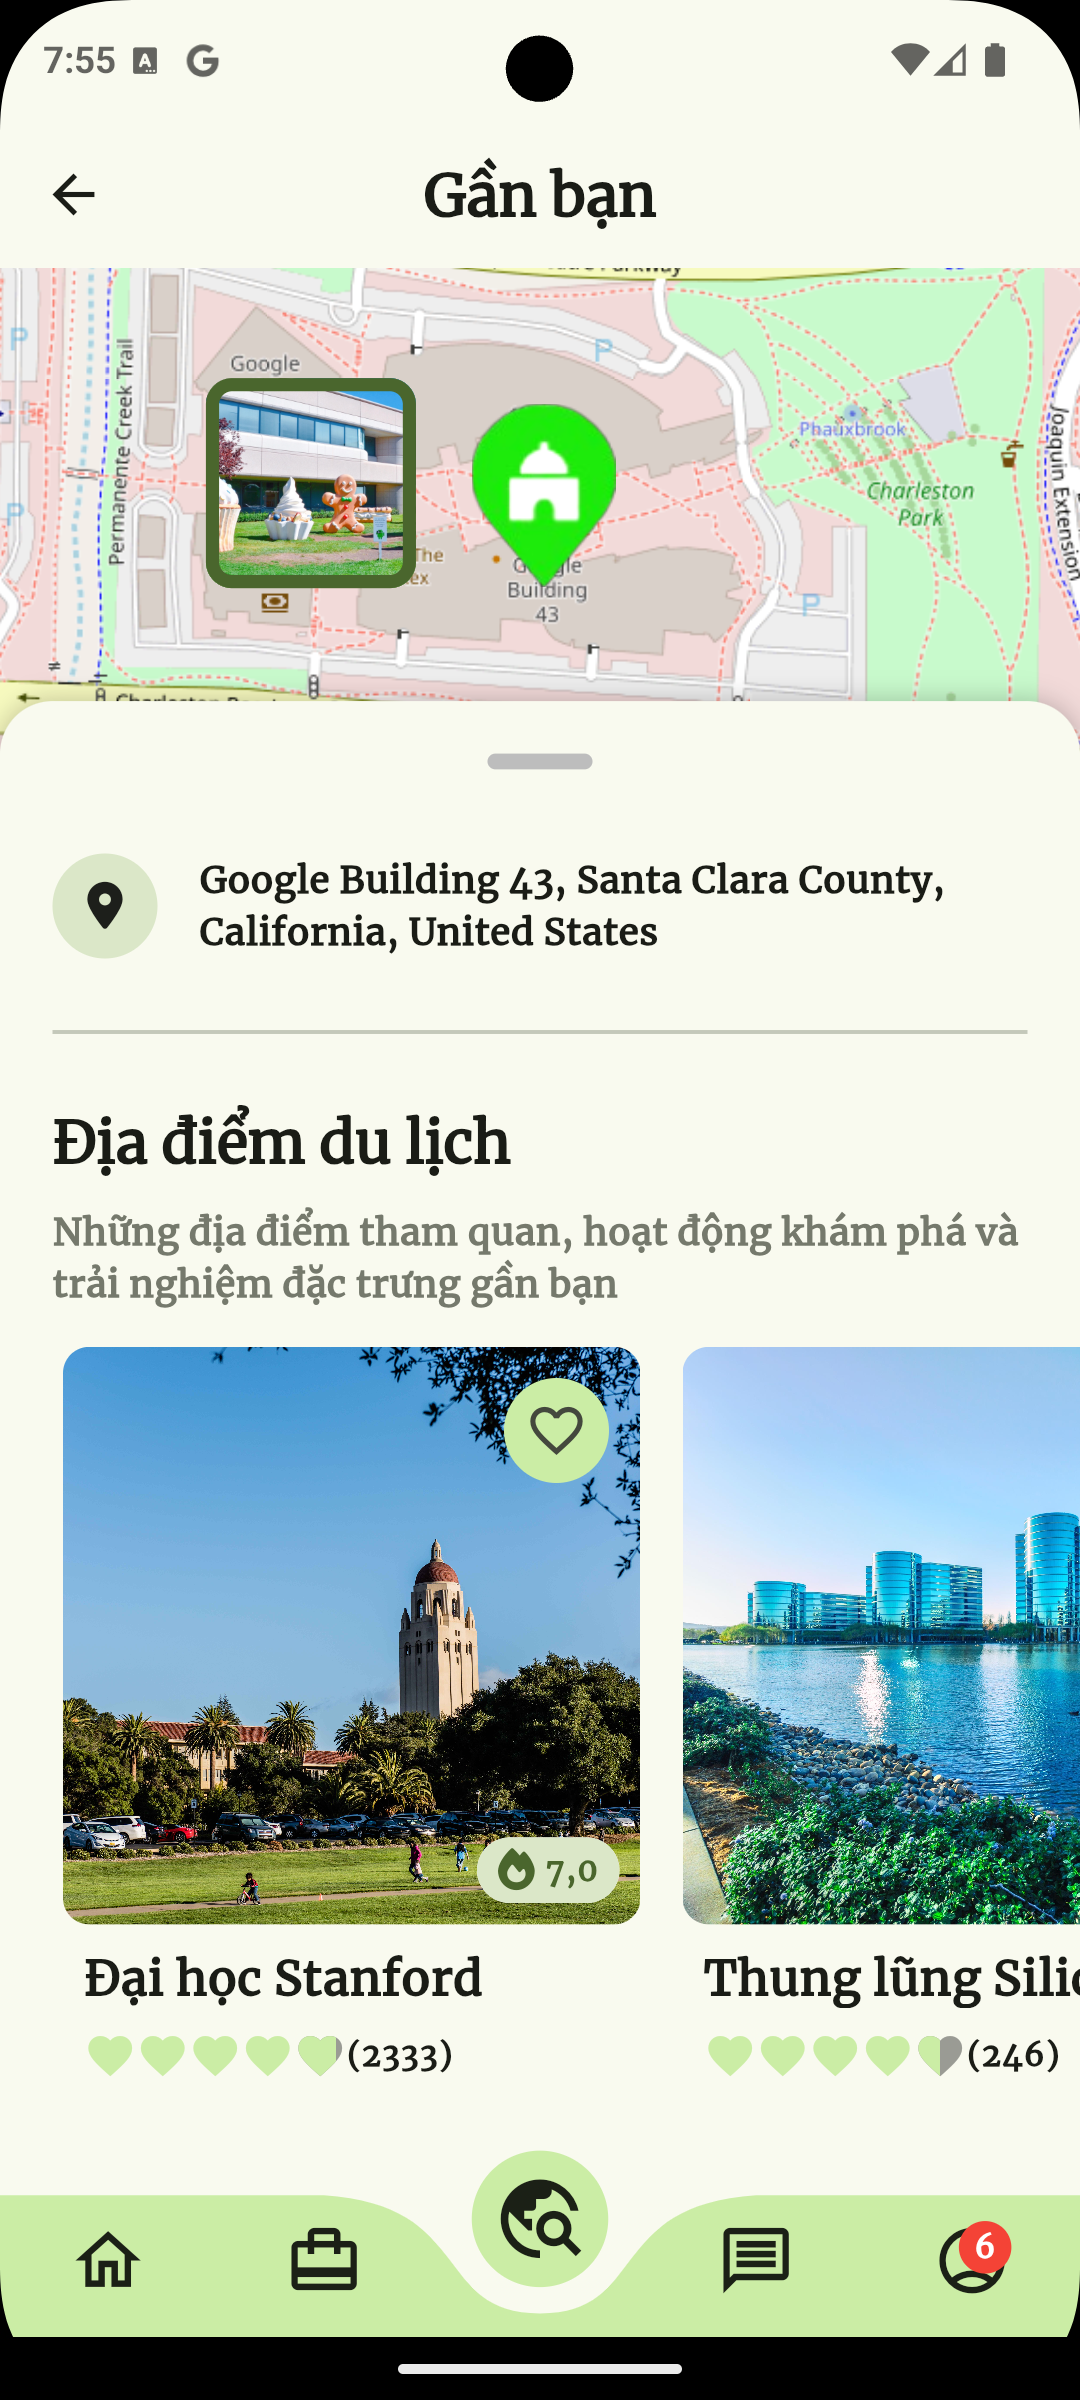
\includegraphics[height=10cm,width=1\linewidth]{figures/c4/system_func/nearby.png}
        \caption{Địa điểm lân cận}
        \label{fig:func_nearby}
    \end{subfigure}
    \hfill
    \begin{subfigure}{0.326\textwidth}
        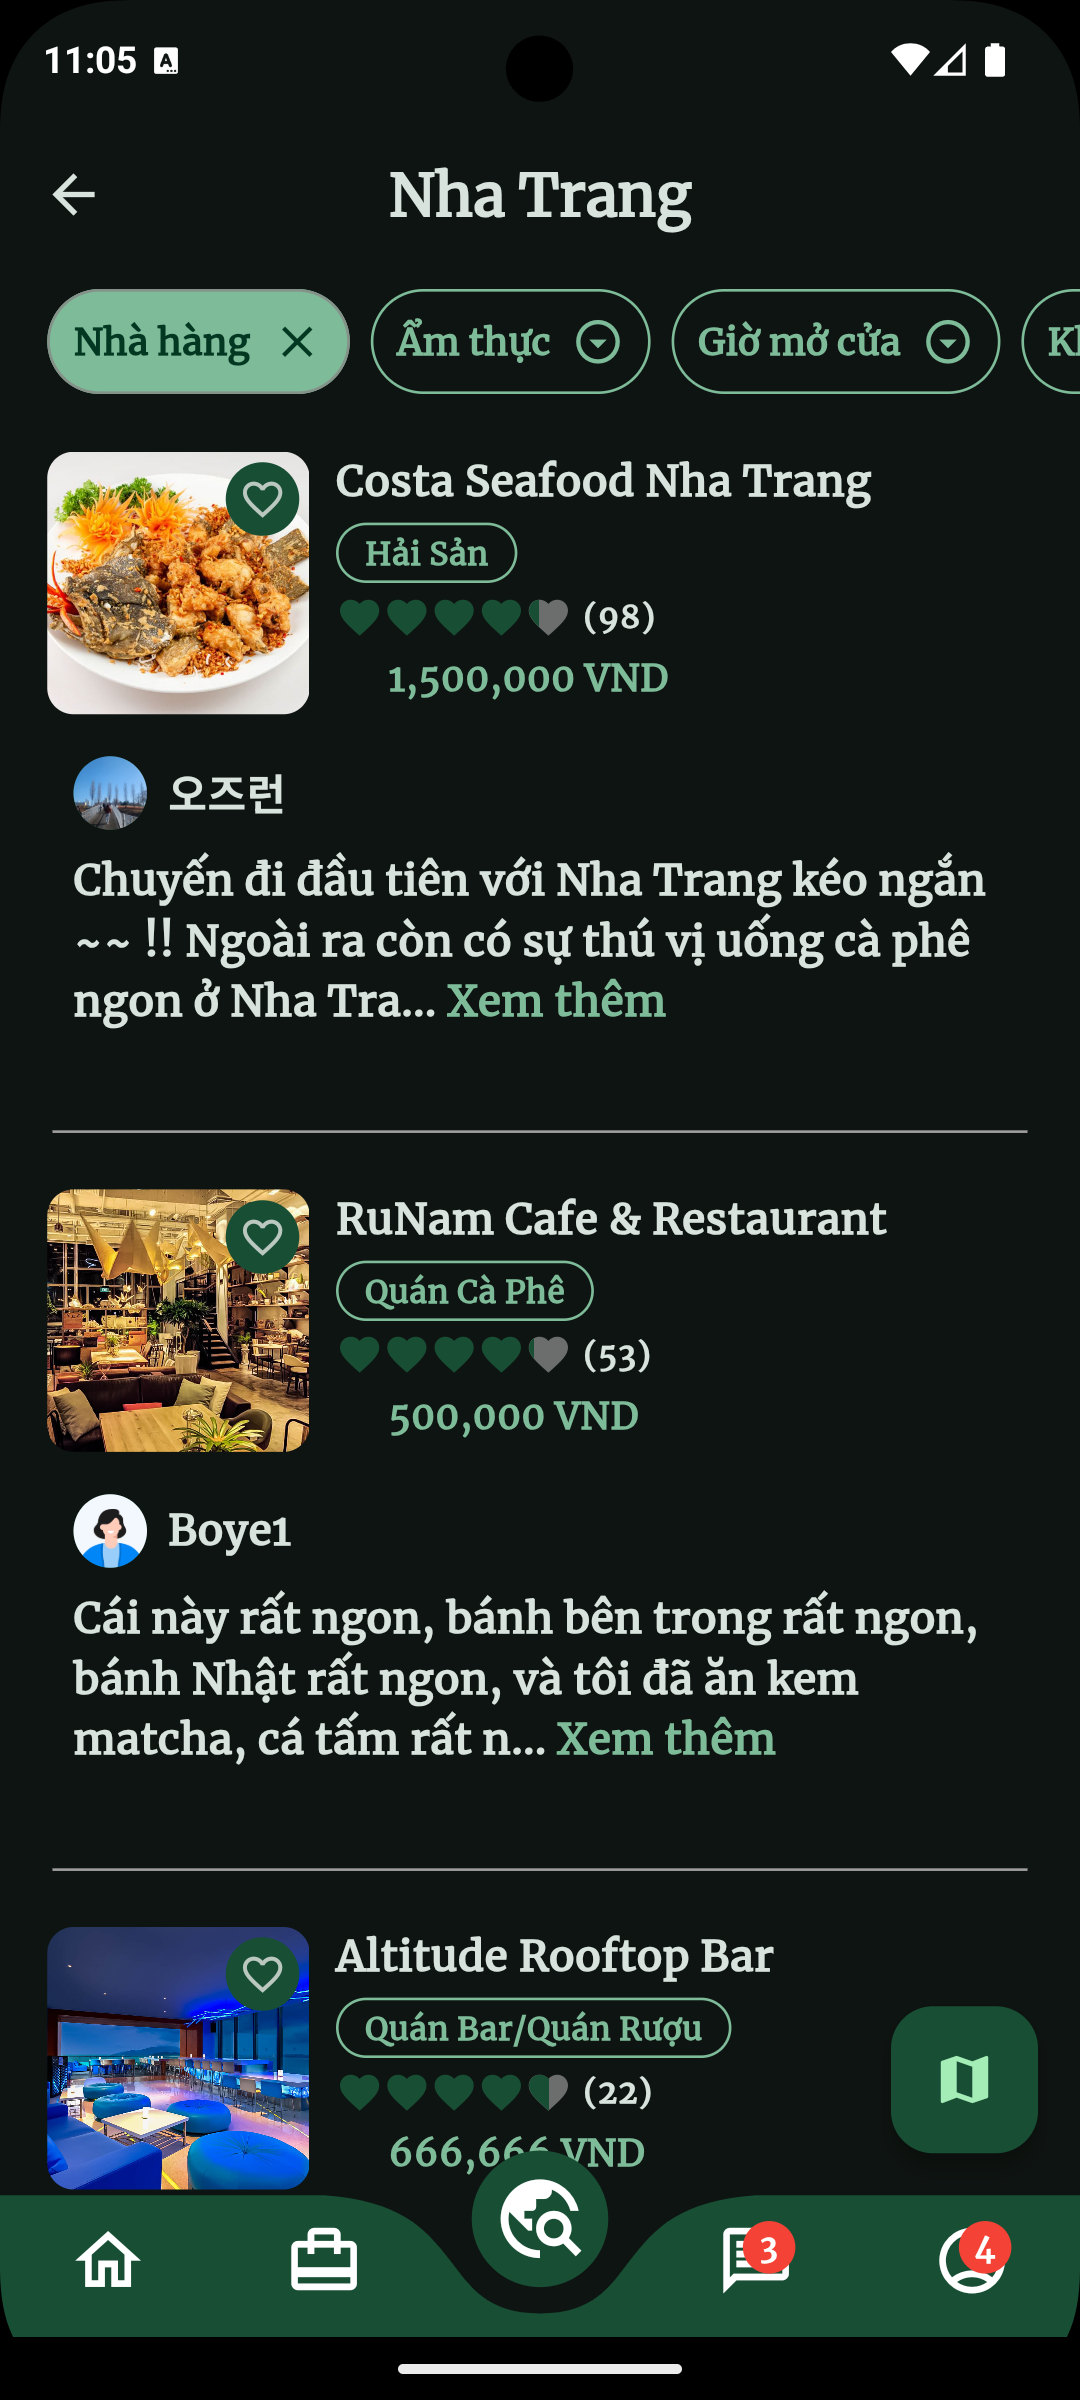
\includegraphics[height=10cm,width=1\linewidth]{figures/c4/system_func/res.png}
        \caption{Lọc địa điểm}
        \label{fig:func_filter_res}
    \end{subfigure}
    \hfill
    \begin{subfigure}{0.326\textwidth}
        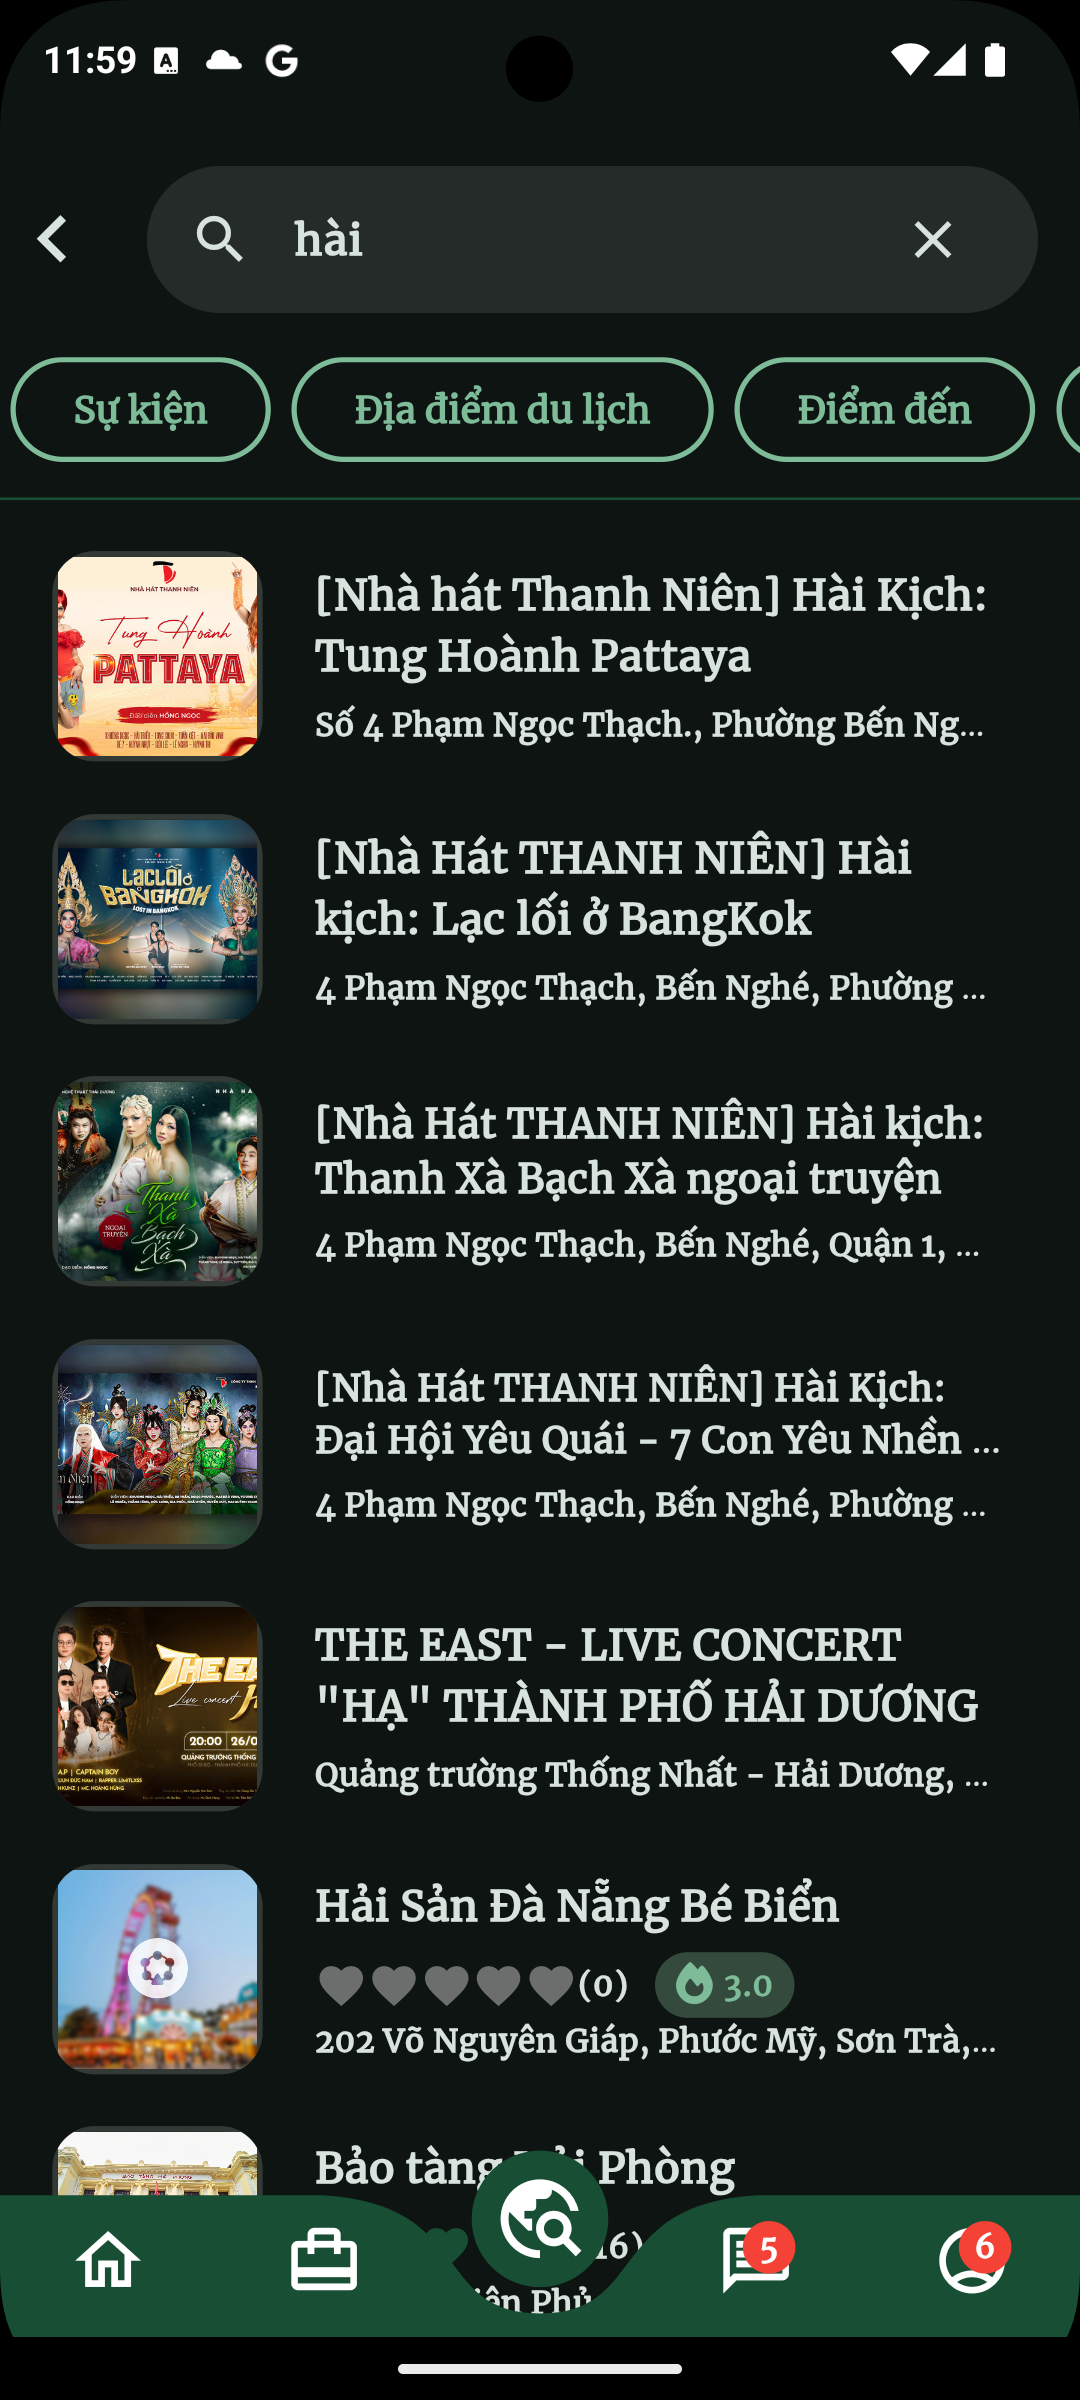
\includegraphics[height=10cm,width=1\linewidth]{figures/c4/system_func/search.png}
        \caption{Tìm kiếm địa điểm}
        \label{fig:func_search_loc}
    \end{subfigure}

    \caption{Các giao diện chính của chức năng Khám phá.}
    \label{fig:explore-screens}
\end{figure}

\subsection{Quản lý Chuyến đi và Lịch trình}
\noindent Người dùng có thể tạo, tham gia và quản lý các chuyến đi. Trong mỗi chuyến đi, người dùng có thể xem và chỉnh sửa thông tin chung (Hình~\ref{fig:func_trip_info}), quản lý danh sách các địa điểm/dịch vụ đã lưu để cân nhắc (Hình~\ref{fig:func_saved_service}), và quản lý thành viên tham gia (Hình~\ref{fig:func_manage_member}), như minh họa trong Hình~\ref{fig:trip-management-1}.

\begin{figure}[H]
    \centering
    \begin{subfigure}{0.326\textwidth}
        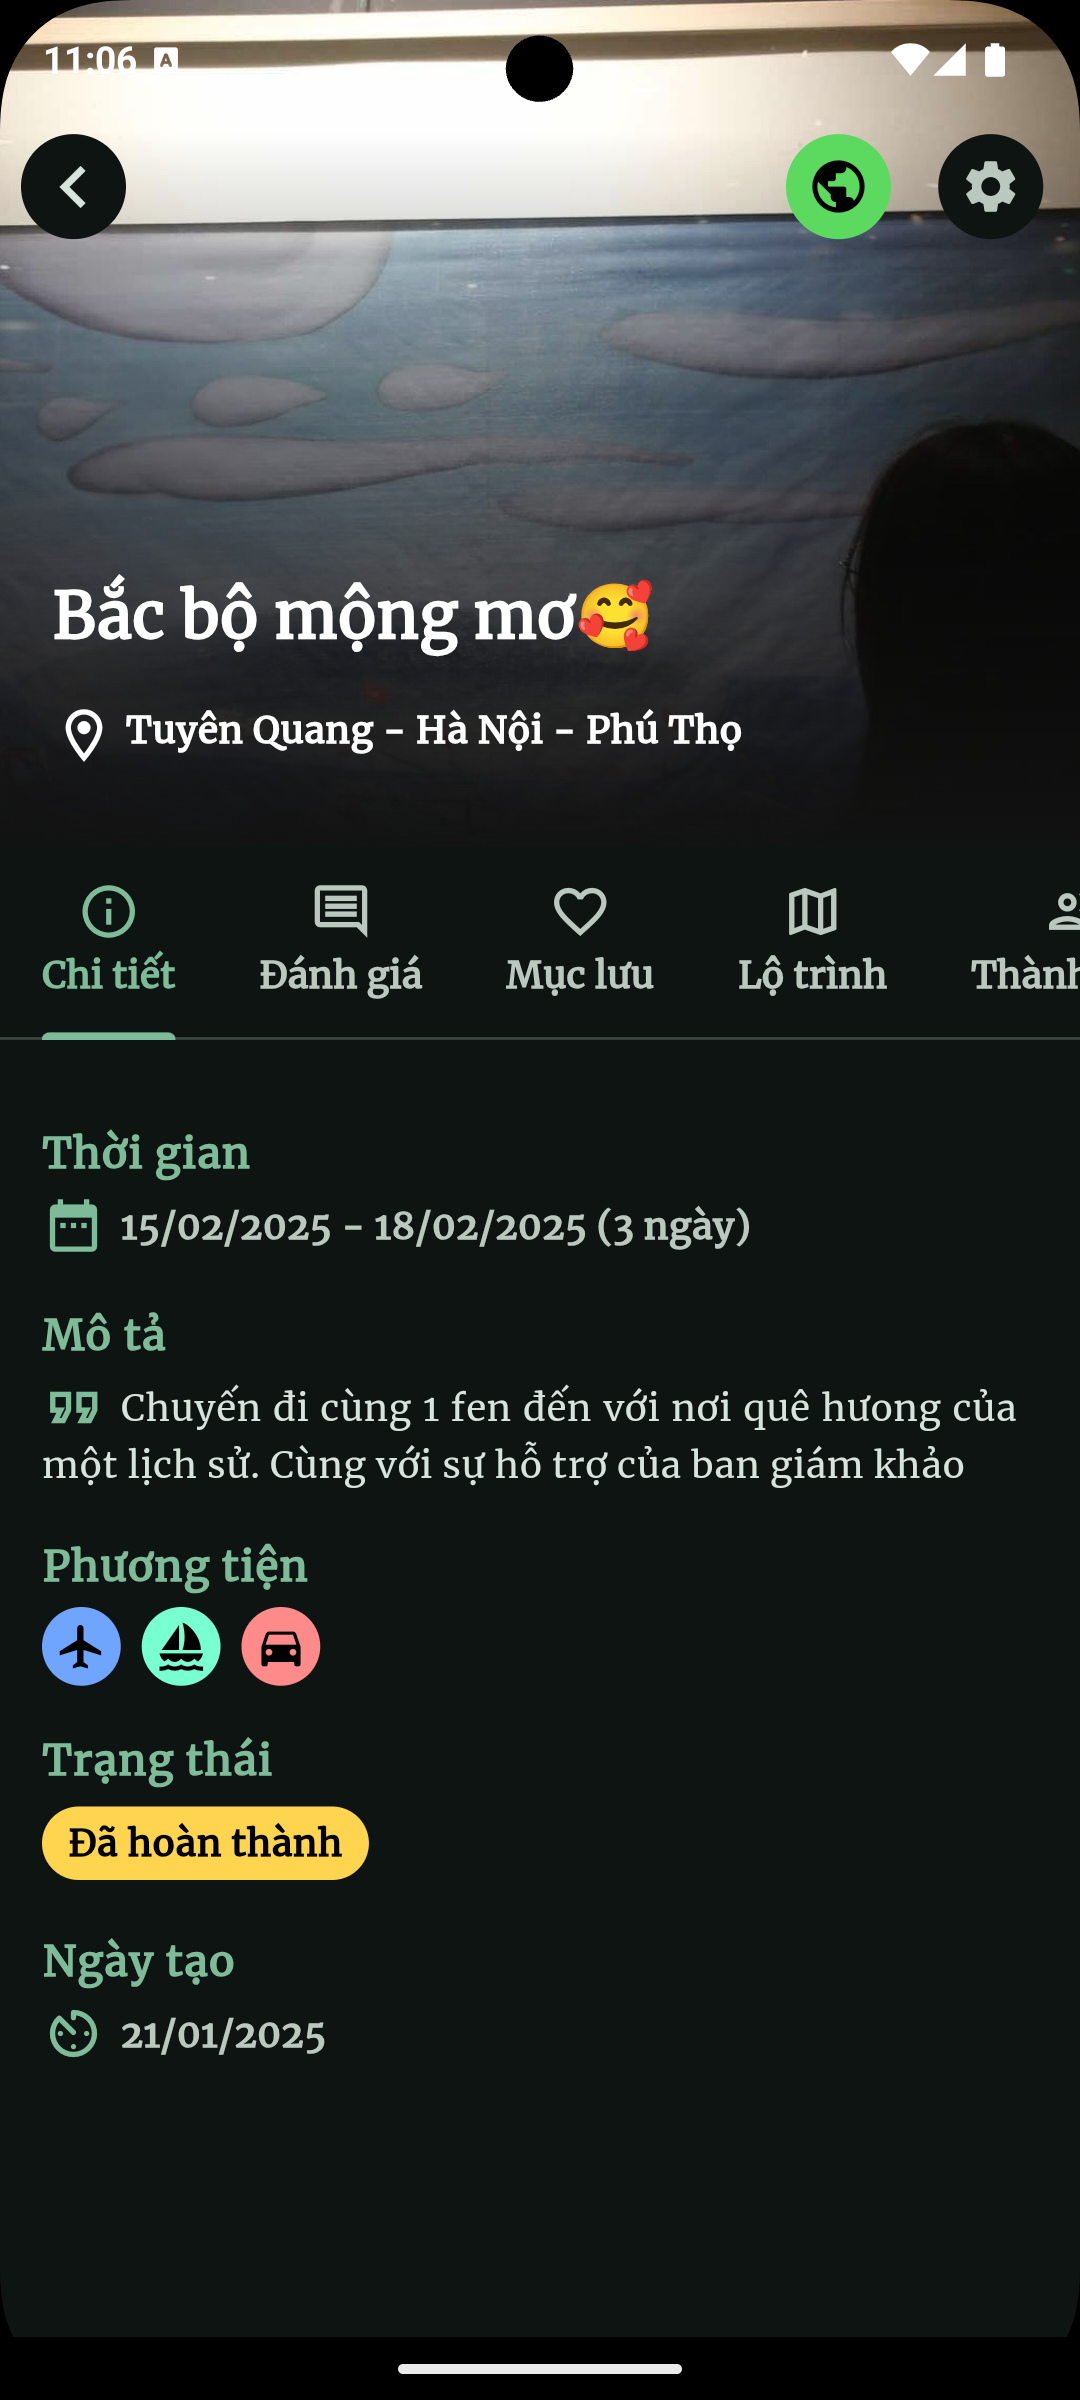
\includegraphics[width=1\linewidth]{figures/c4/system_func/tripinfo.png}
        \caption{Thông tin chuyến đi}
        \label{fig:func_trip_info}
    \end{subfigure}
    \hfill
    \begin{subfigure}{0.326\textwidth}
        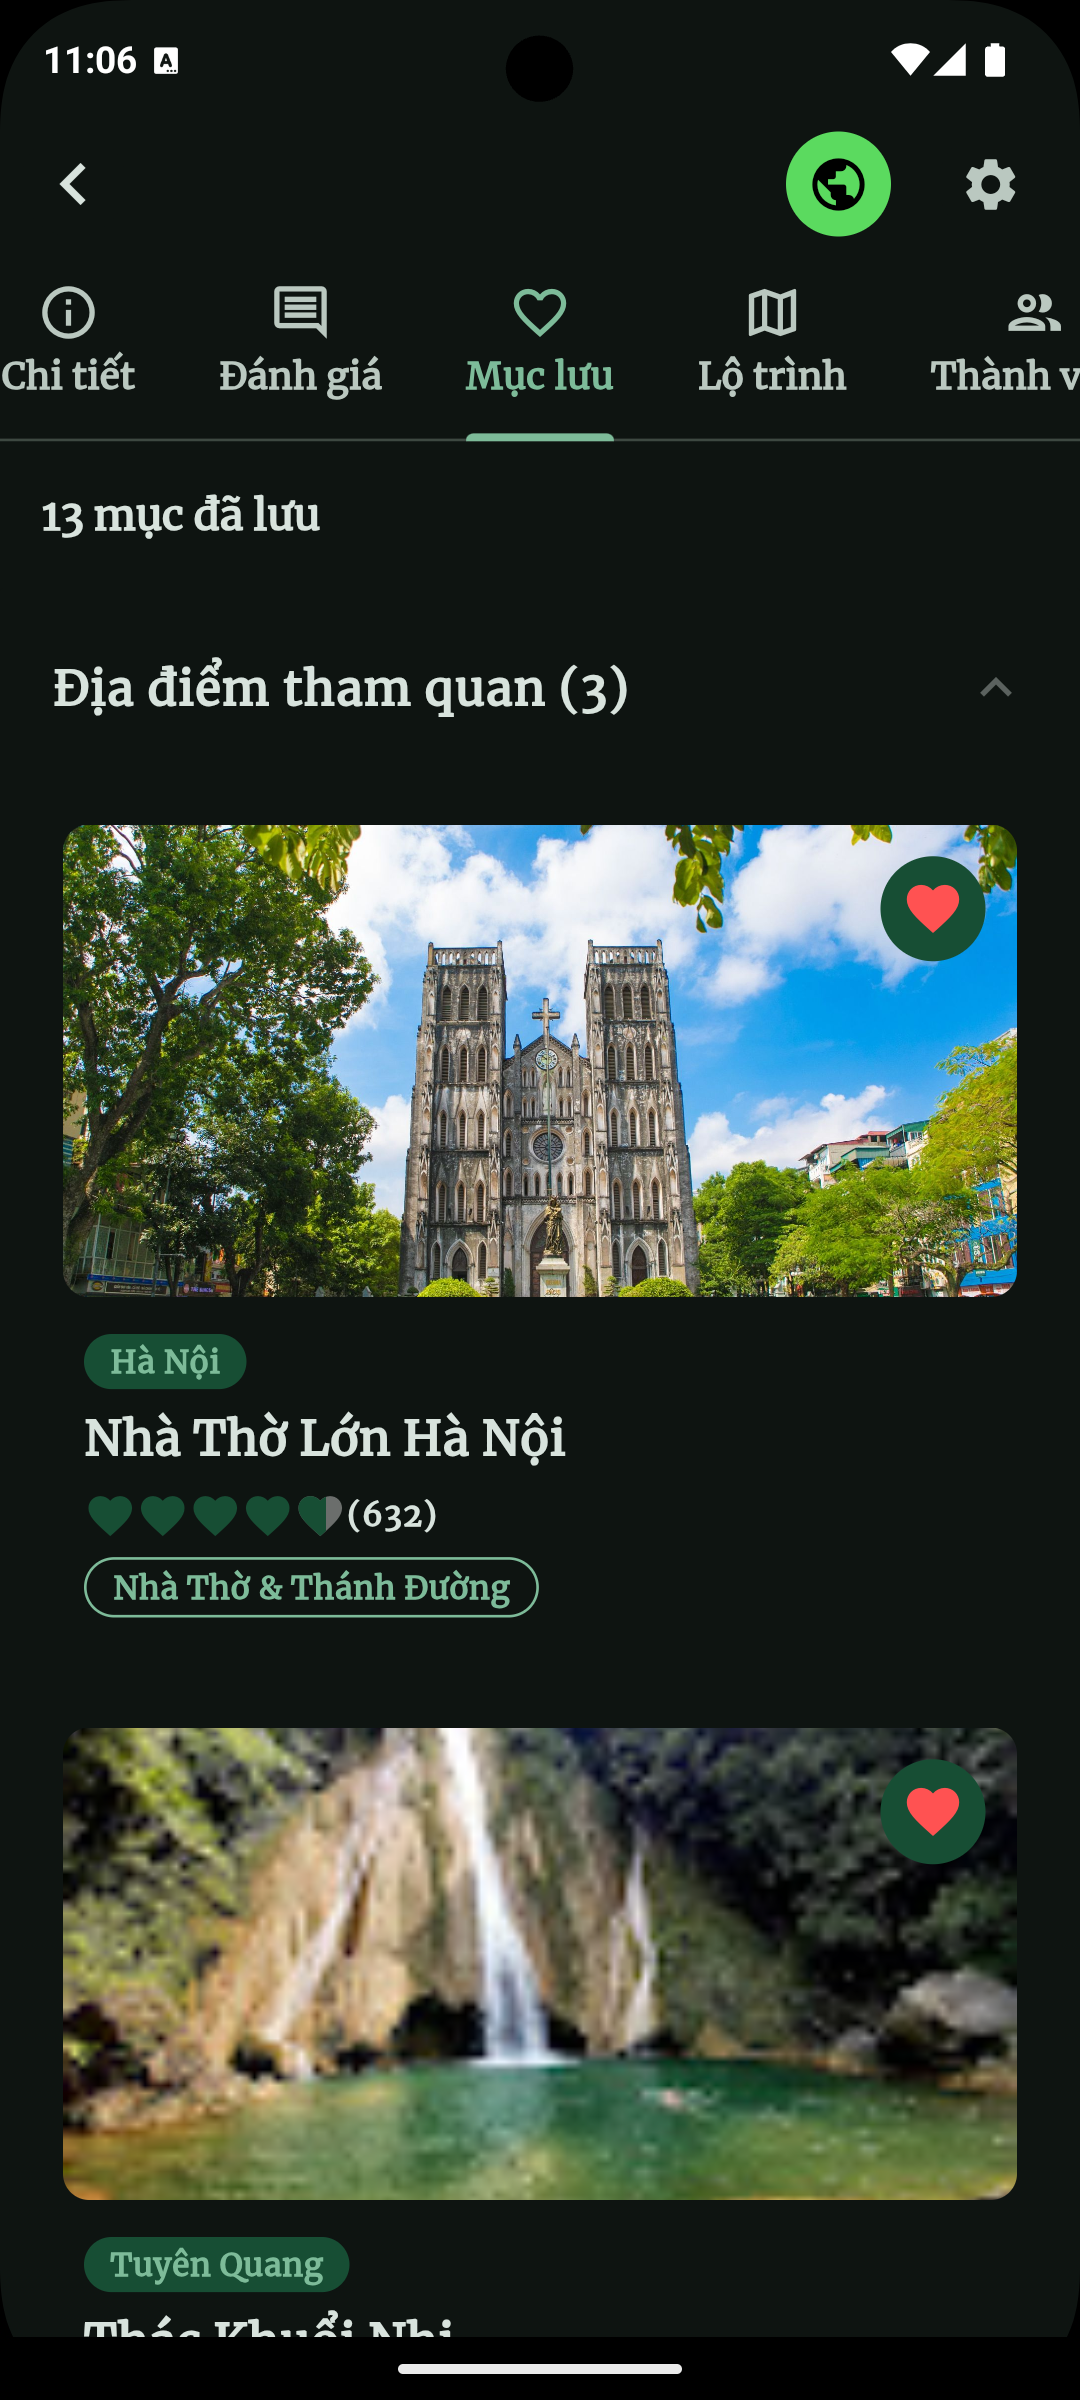
\includegraphics[width=1\linewidth]{figures/c4/system_func/save_service.png}
        \caption{Địa điểm đã lưu}
        \label{fig:func_saved_service}
    \end{subfigure}
    \hfill
    \begin{subfigure}{0.326\textwidth}
        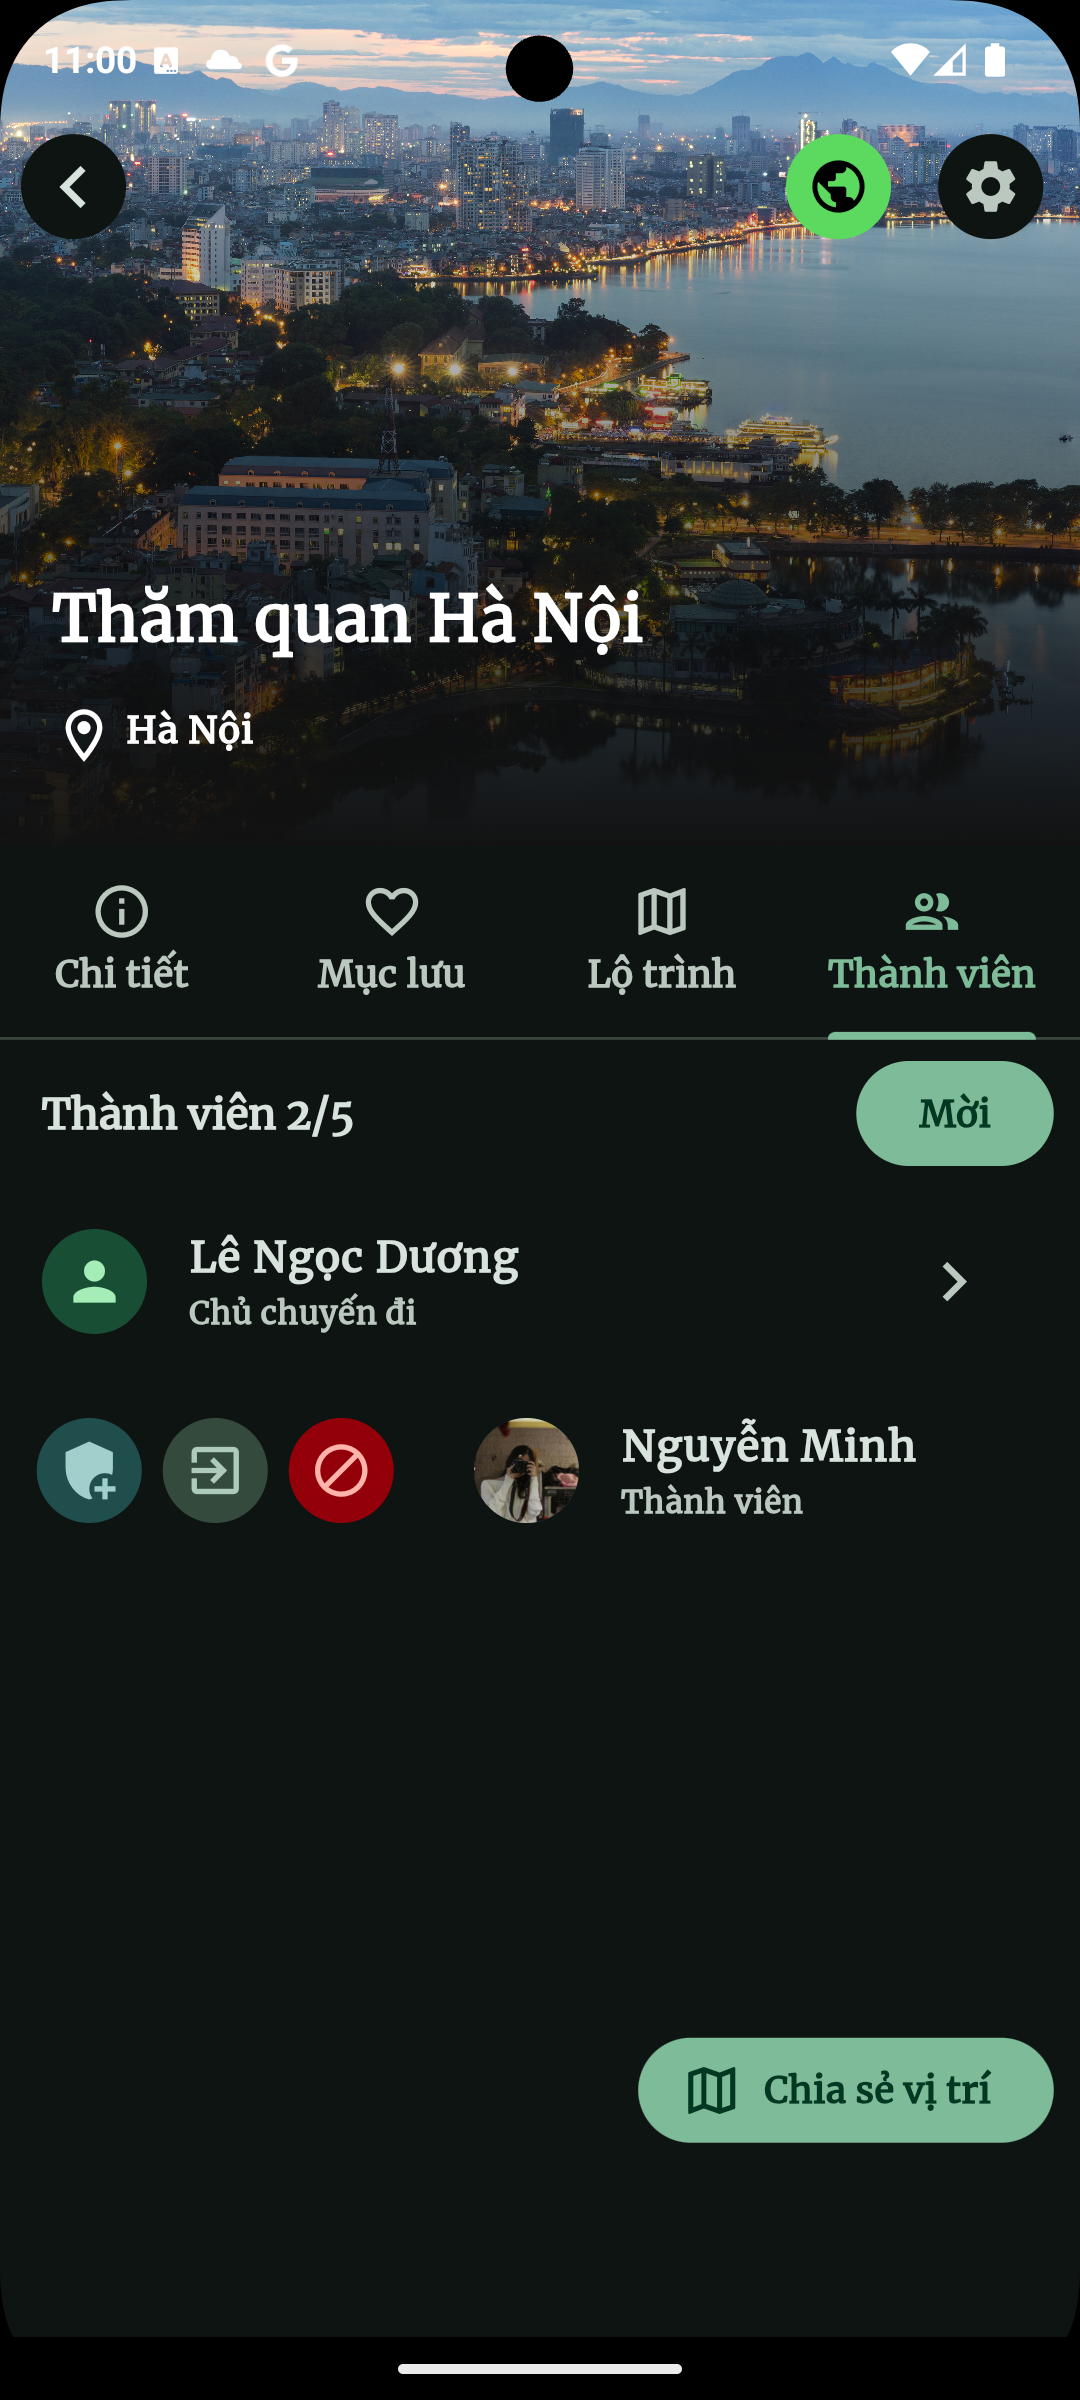
\includegraphics[width=1\linewidth]{figures/c4/system_func/manage_member.png}
        \caption{Quản lý thành viên}
        \label{fig:func_manage_member}
    \end{subfigure}
    \caption{Giao diện quản lý thông tin chuyến đi.}
    \label{fig:trip-management-1}
\end{figure}

\noindent \noindent Chức năng cốt lõi là tạo và quản lý lịch trình chi tiết cho chuyến đi (Hình~\ref{fig:trip-management-2}). Người dùng có thể xem danh sách các mục trong lịch trình (Hình~\ref{fig:func_itinerary_list}), thêm các hoạt động mới với thời gian, địa điểm cụ thể (Hình~\ref{fig:func_add_itinerary}), và xem trực quan lịch trình theo ngày trên bản đồ (Hình~\ref{fig:func_itinerary_map}).

\begin{figure}[H]
    \centering
    \begin{subfigure}{0.326\textwidth}
        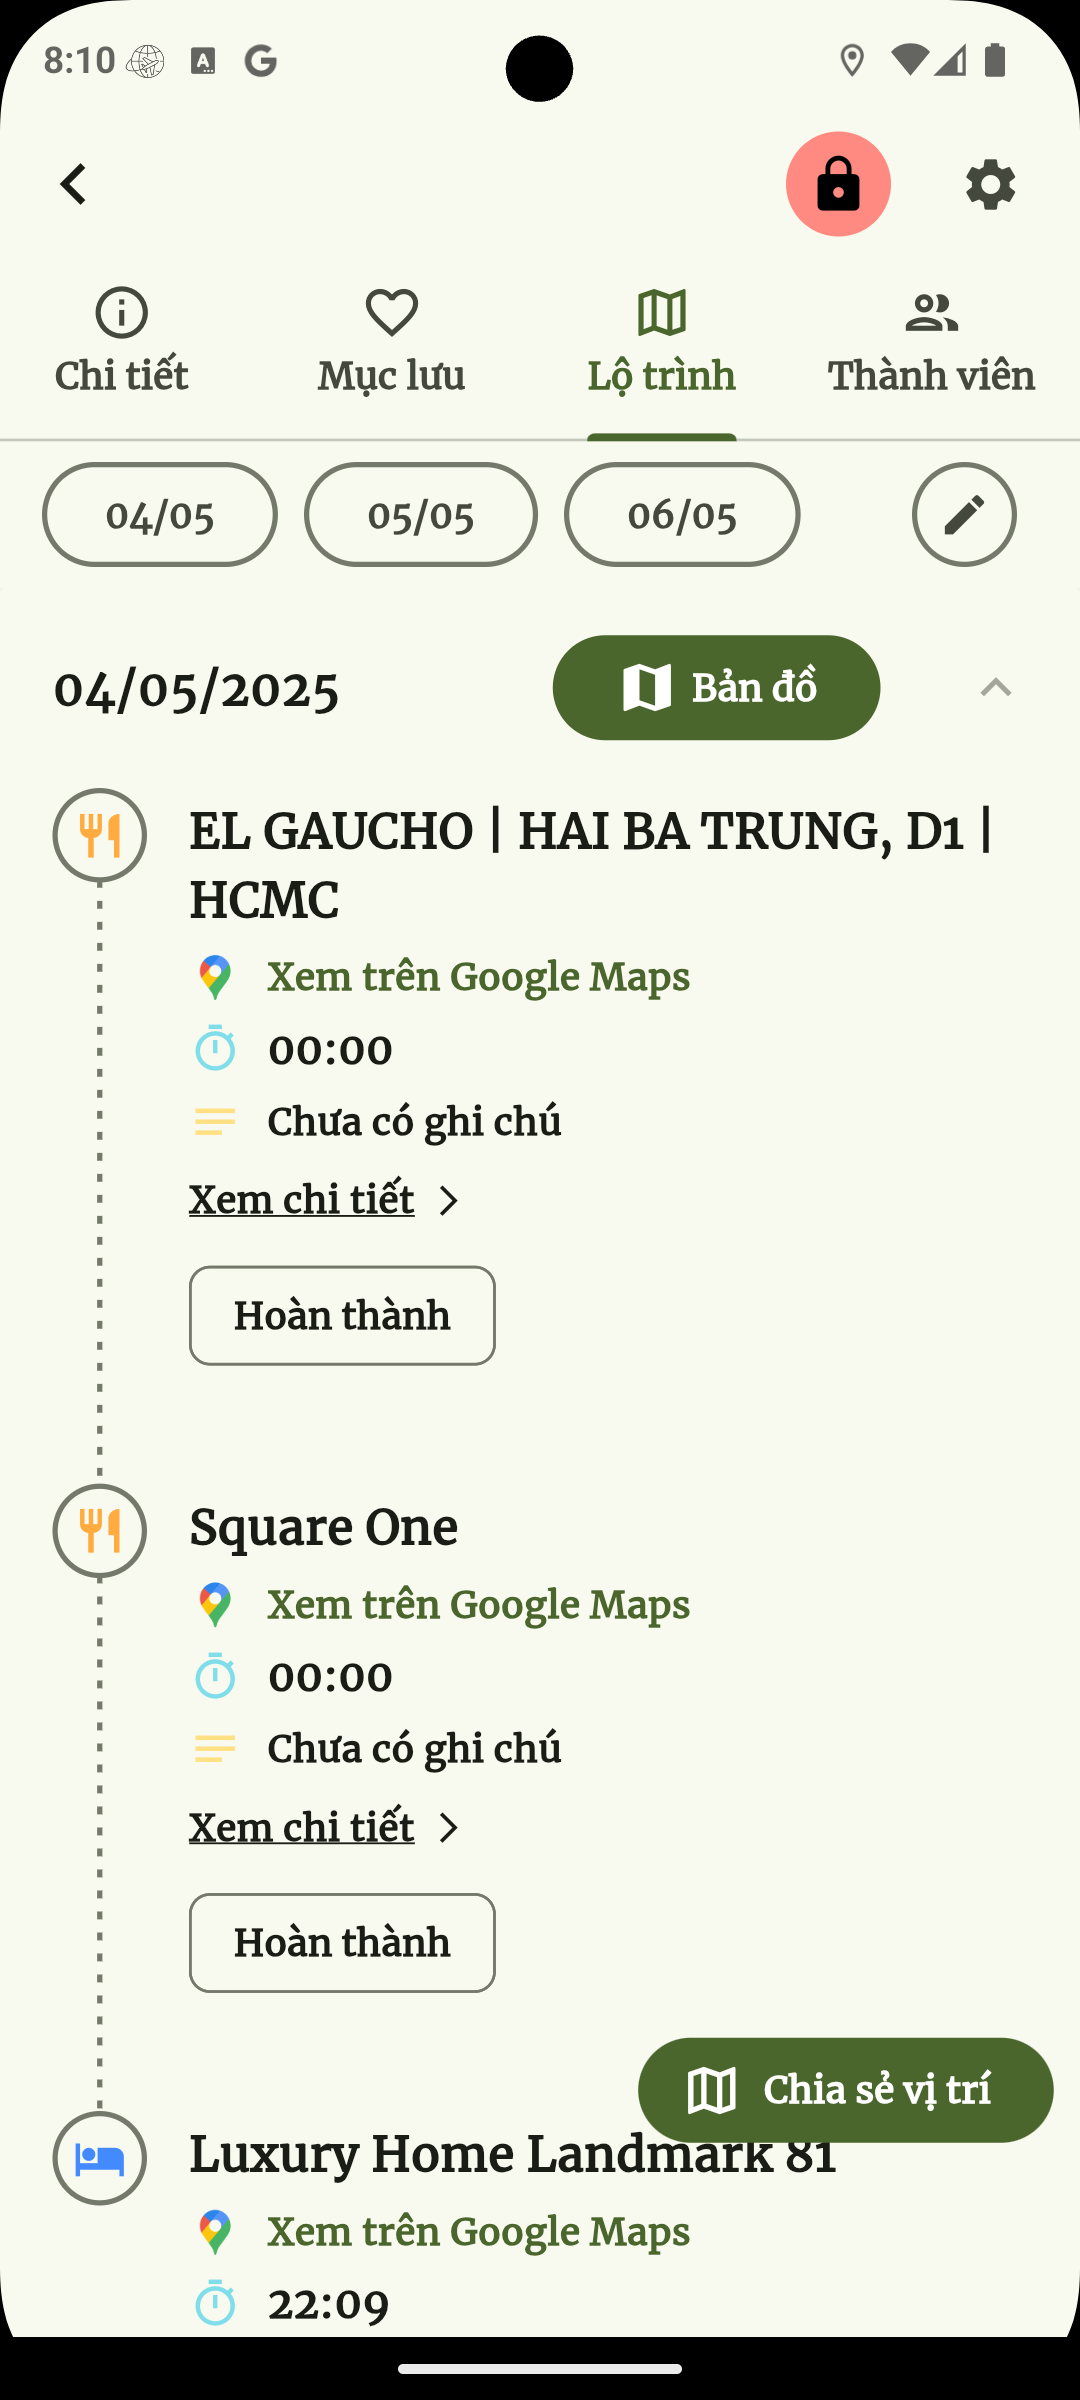
\includegraphics[width=1\linewidth]{figures/c4/system_func/itinerary.png}
        \caption{Danh sách lịch trình}
        \label{fig:func_itinerary_list}
    \end{subfigure}
    \hfill
    \begin{subfigure}{0.326\textwidth}
        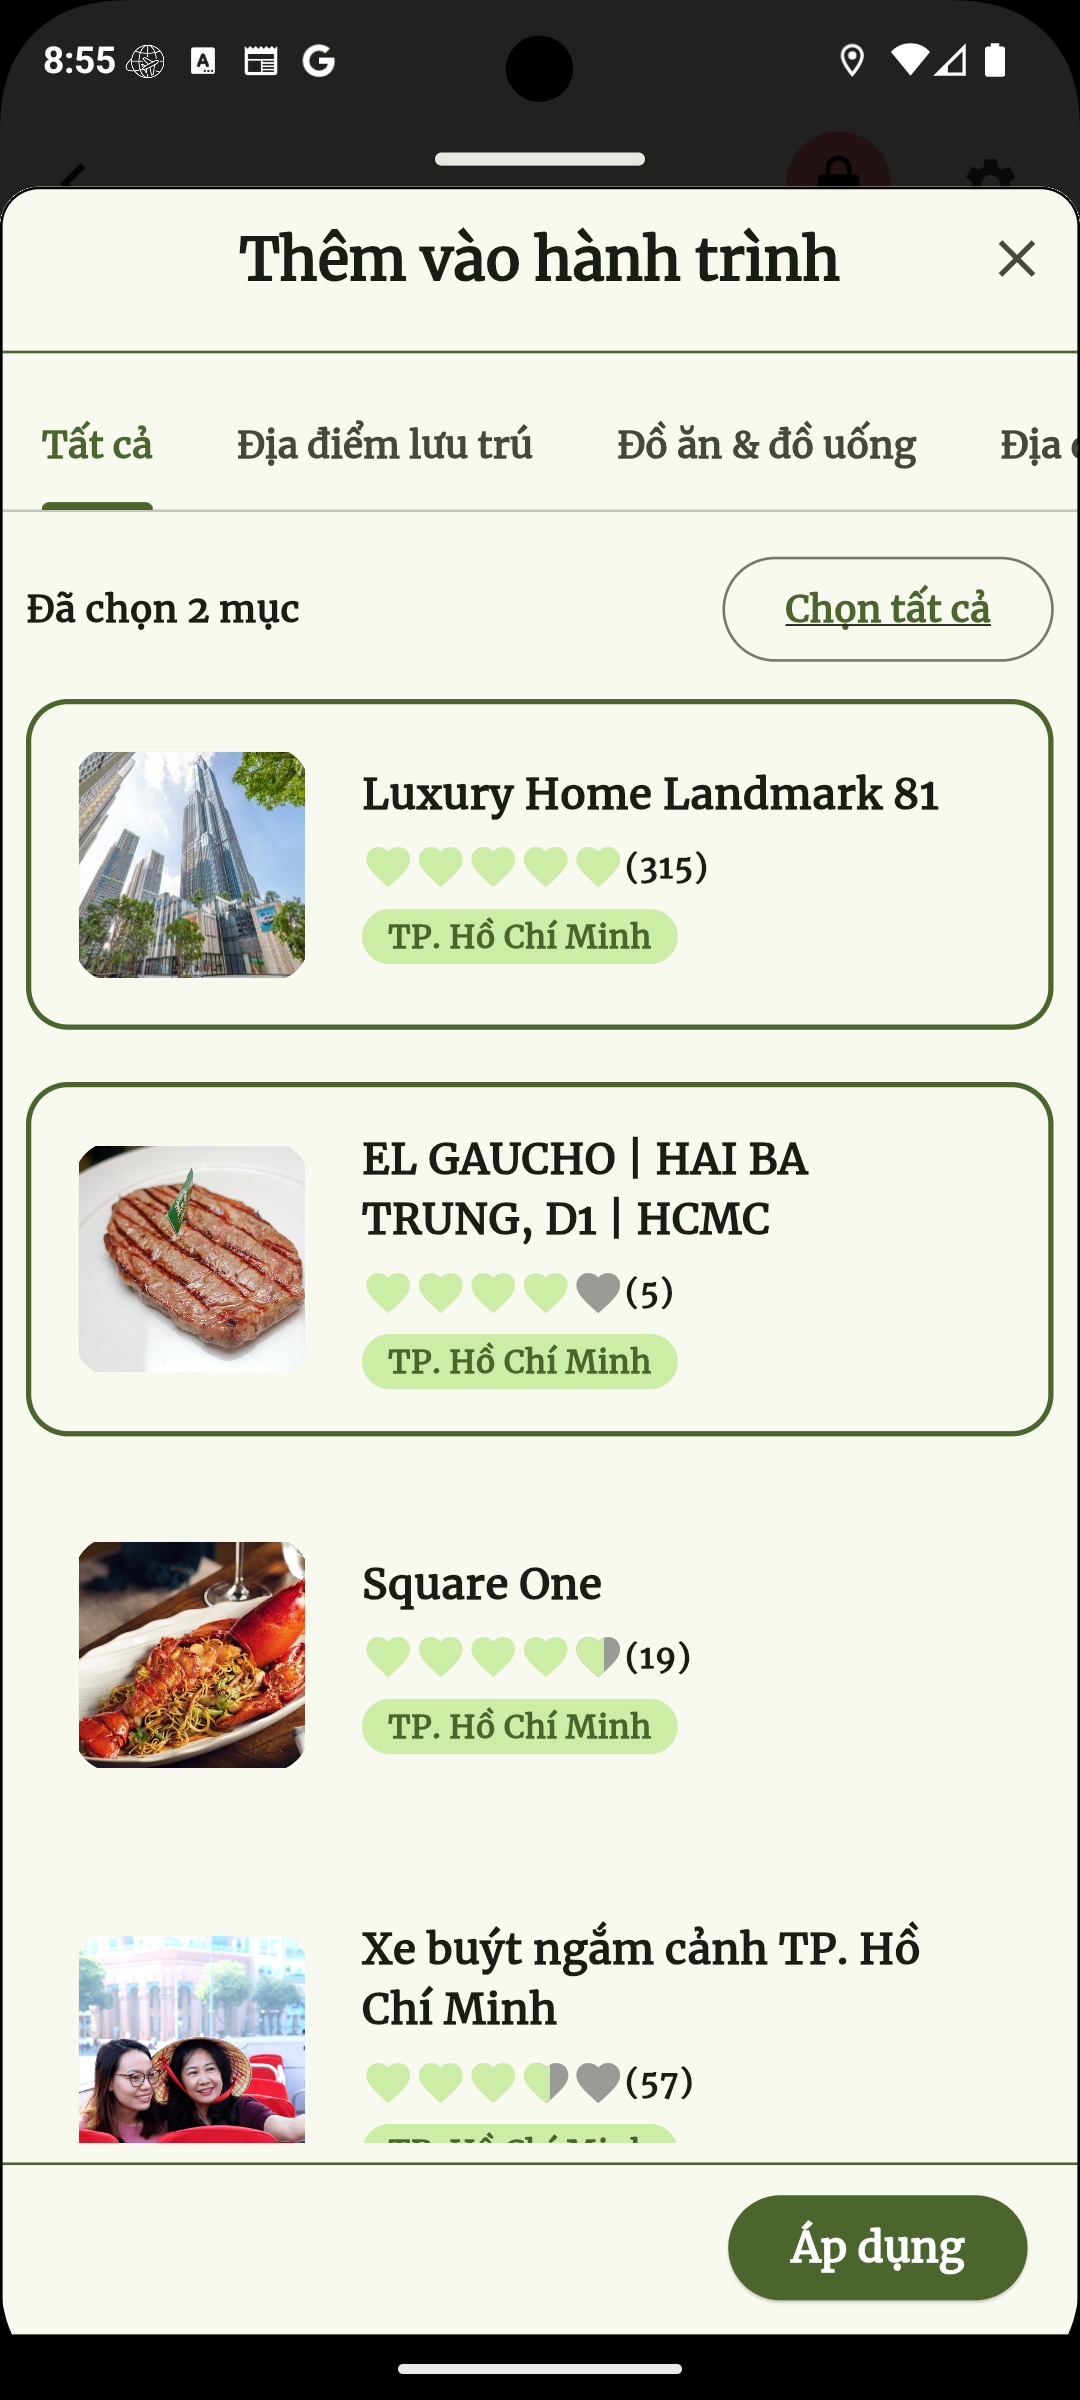
\includegraphics[width=1\linewidth]{figures/c4/system_func/itinerary_1.png}
        \caption{Thêm mục lịch trình}
        \label{fig:func_add_itinerary}
    \end{subfigure}
    \hfill
    \begin{subfigure}{0.326\textwidth}
        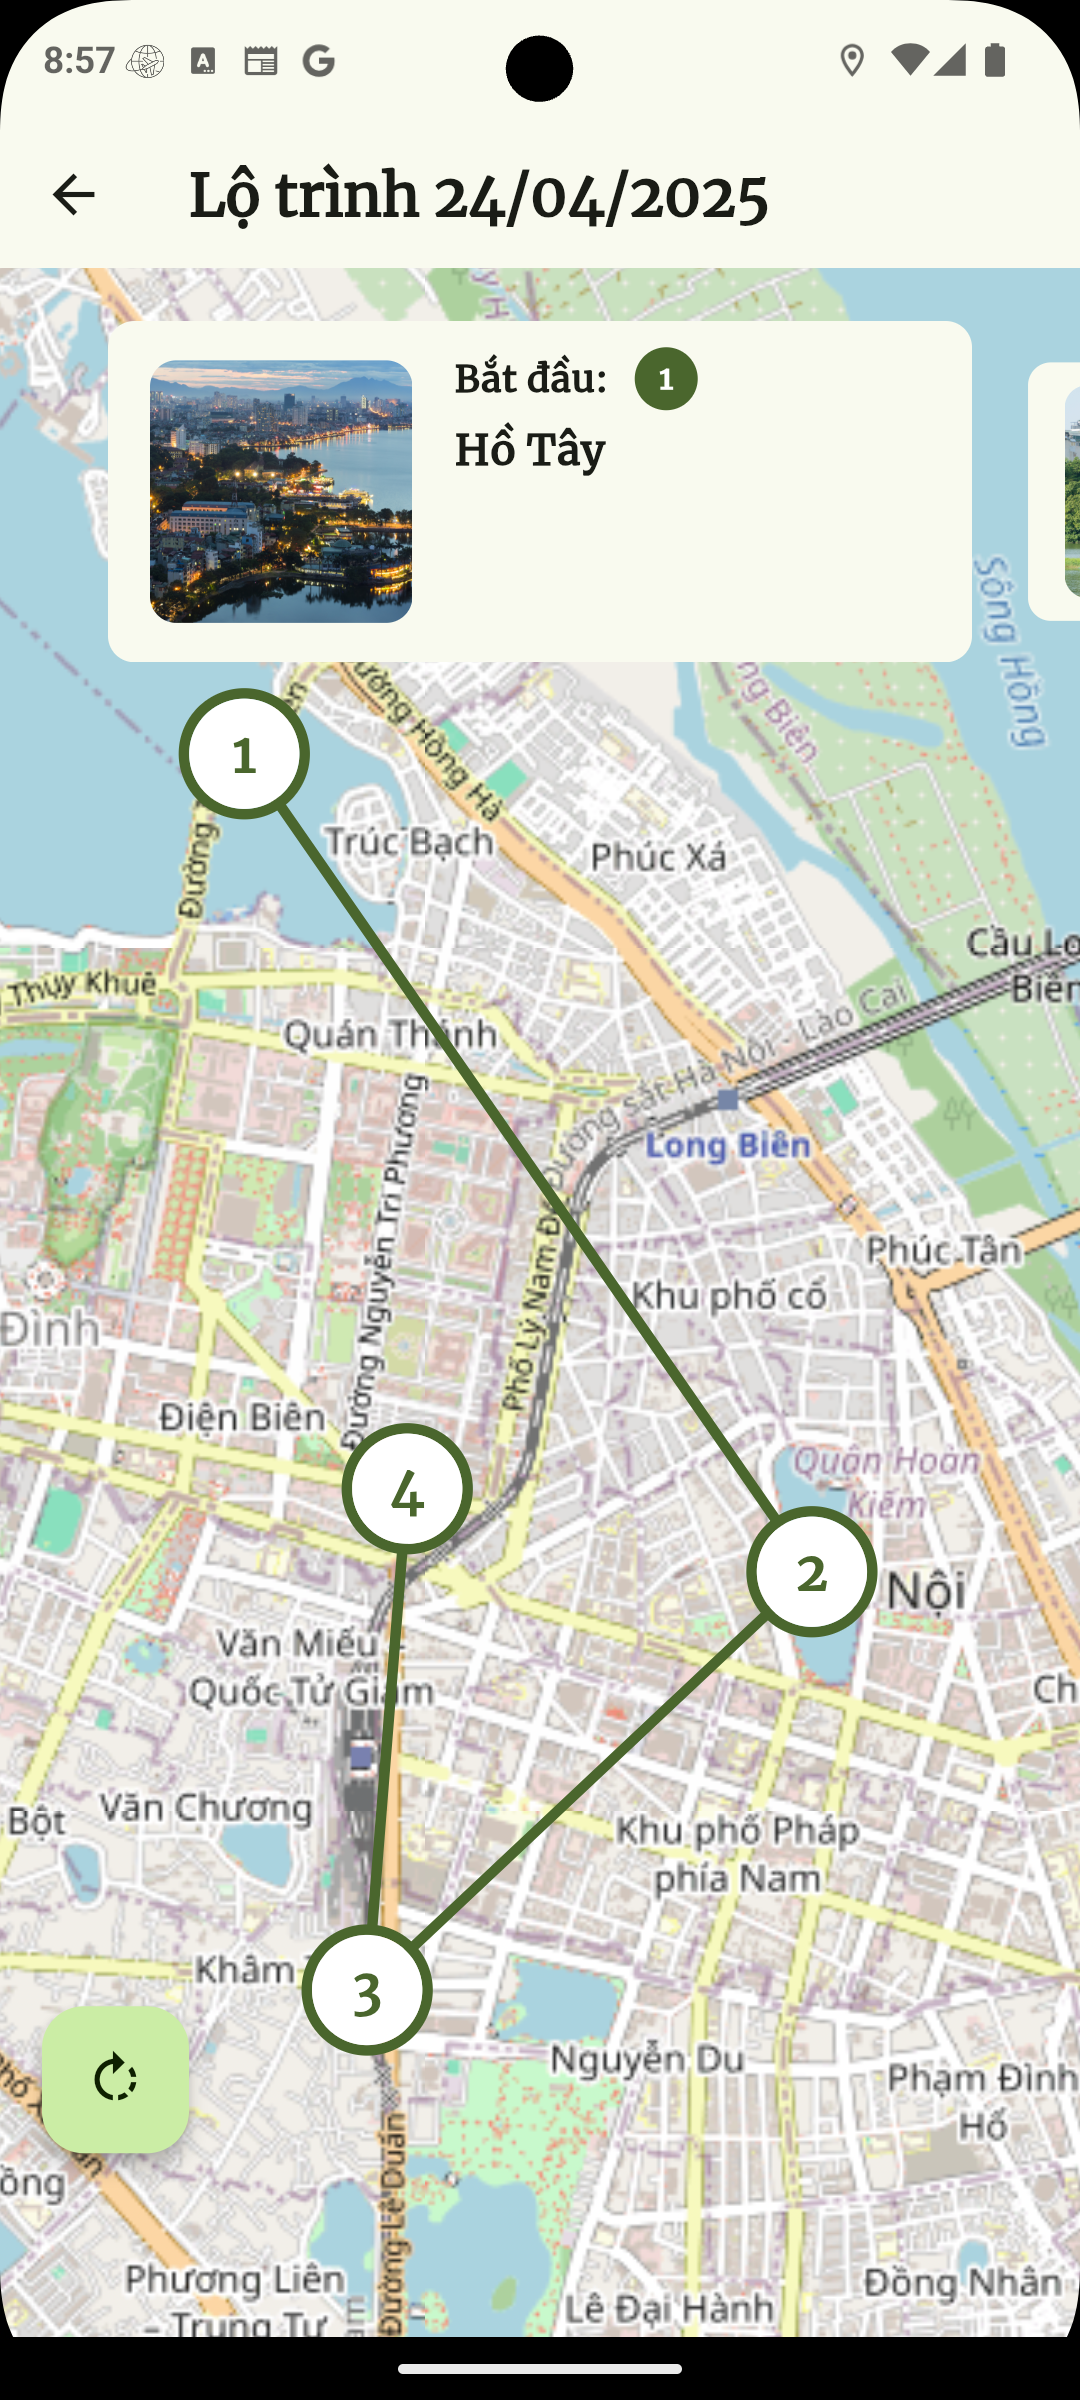
\includegraphics[width=1\linewidth]{figures/c4/system_func/itinerary_map.png}
        \caption{Xem lịch trình trên bản đồ}
        \label{fig:func_itinerary_map}
    \end{subfigure}
    \caption{Giao diện quản lý lịch trình chuyến đi.}
    \label{fig:trip-management-2}
\end{figure}

\noindent \noindent Tùy thuộc vào trạng thái chuyến đi, hệ thống cung cấp các tính năng phù hợp (Hình~\ref{fig:trip-management-3}). Khi chuyến đi ``đang diễn ra", thành viên có thể chia sẻ vị trí thời gian thực (Hình~\ref{fig:func_share_loc}) và đánh dấu hoàn thành các mục lịch trình. Sau khi chuyến đi kết thúc, người dùng có thể đánh giá chung về chuyến đi (Hình~\ref{fig:func_trip_rating}) và đánh giá các thành viên khác (Hình~\ref{fig:func_member_rating}).

\begin{figure}[H]
    \centering
    \begin{subfigure}{0.326\textwidth}
        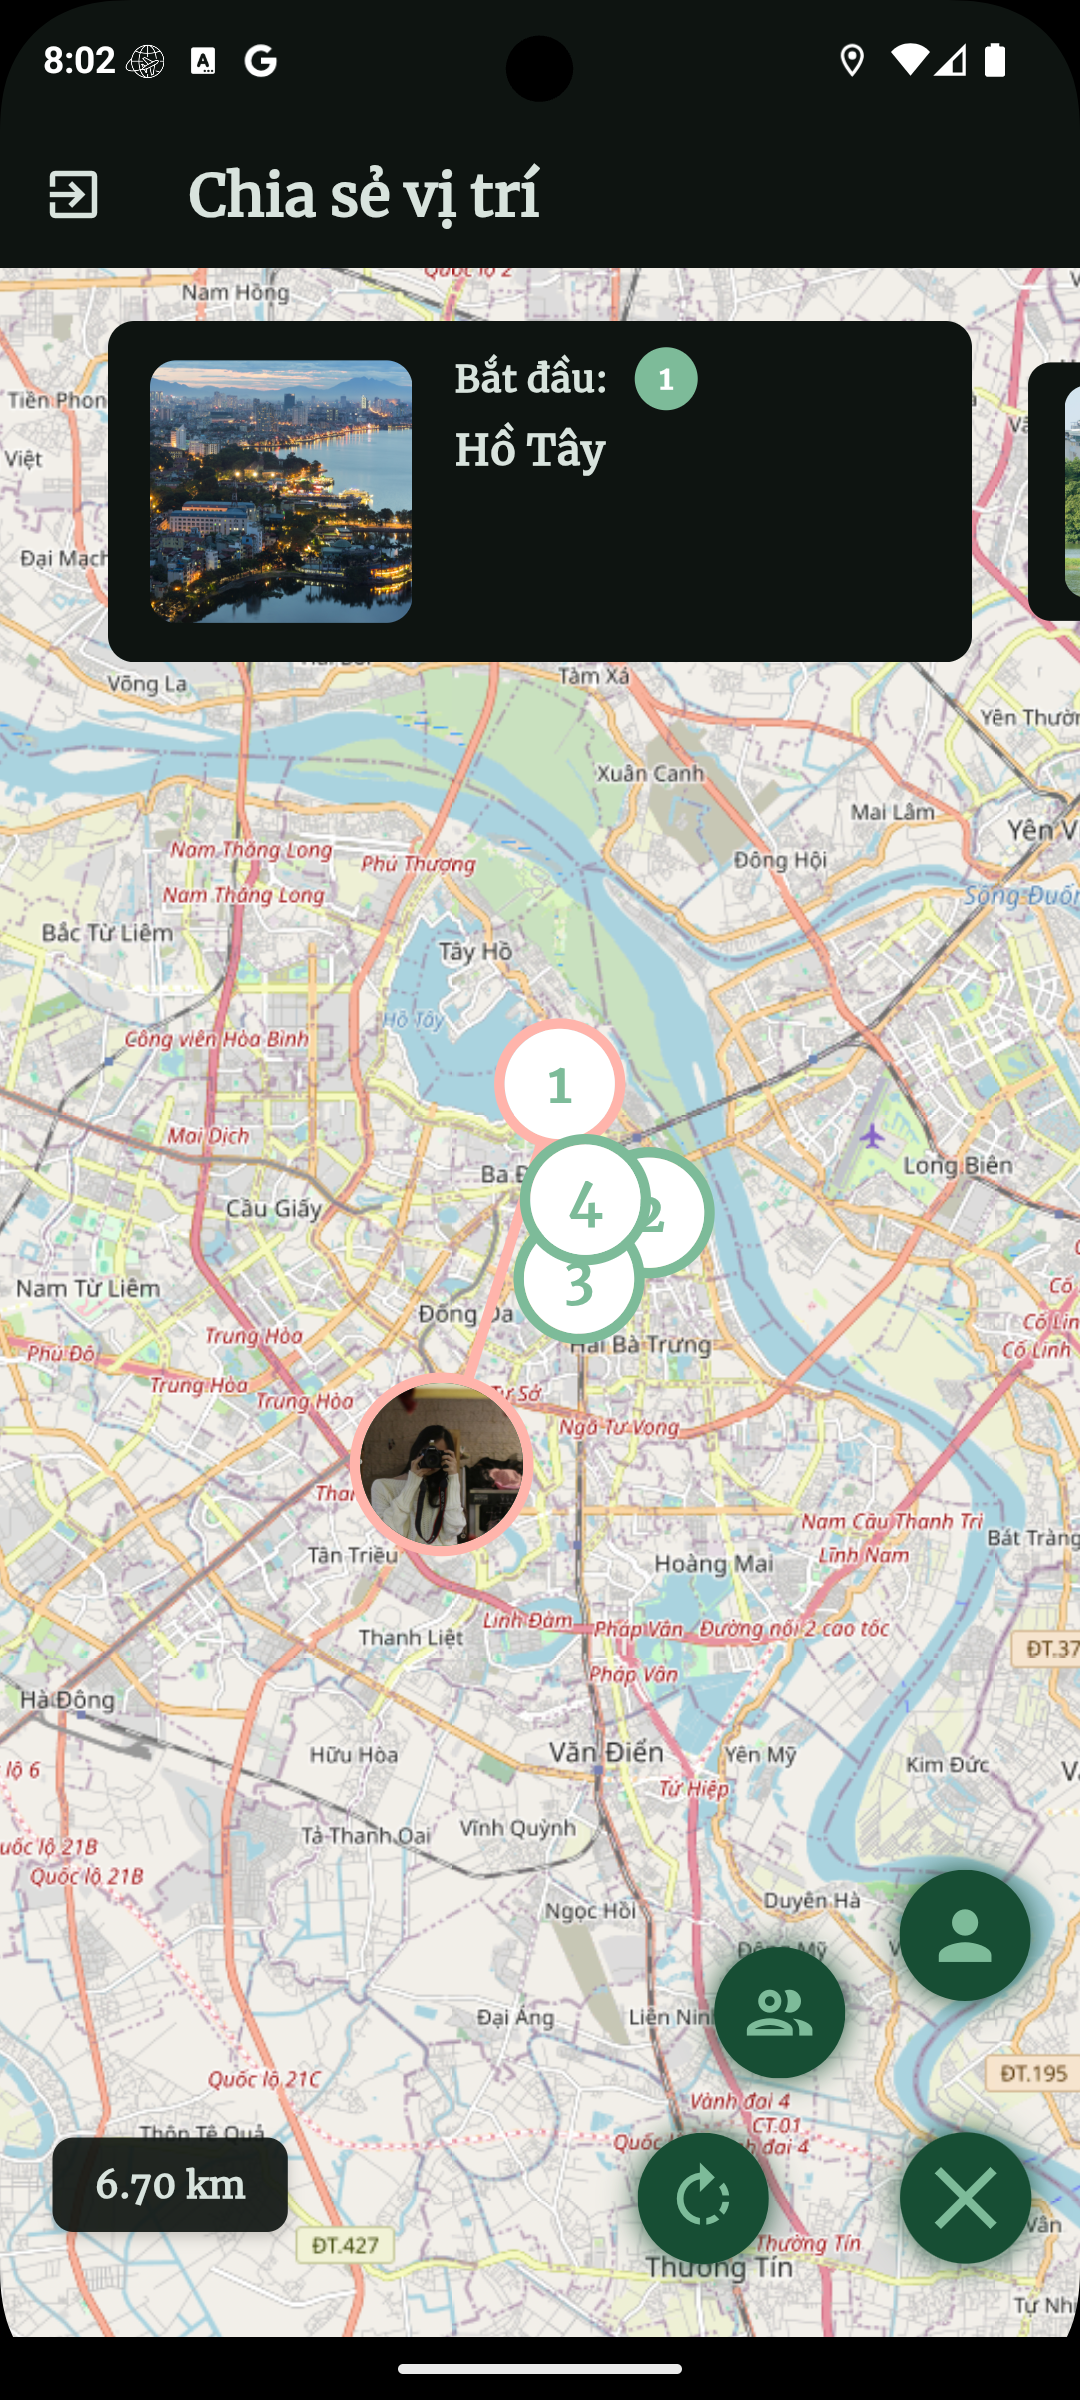
\includegraphics[width=1\linewidth]{figures/c4/system_func/shared_loc_2.png}
        \caption{Chia sẻ vị trí}
        \label{fig:func_share_loc}
    \end{subfigure}
    \hfill
    \begin{subfigure}{0.326\textwidth}
        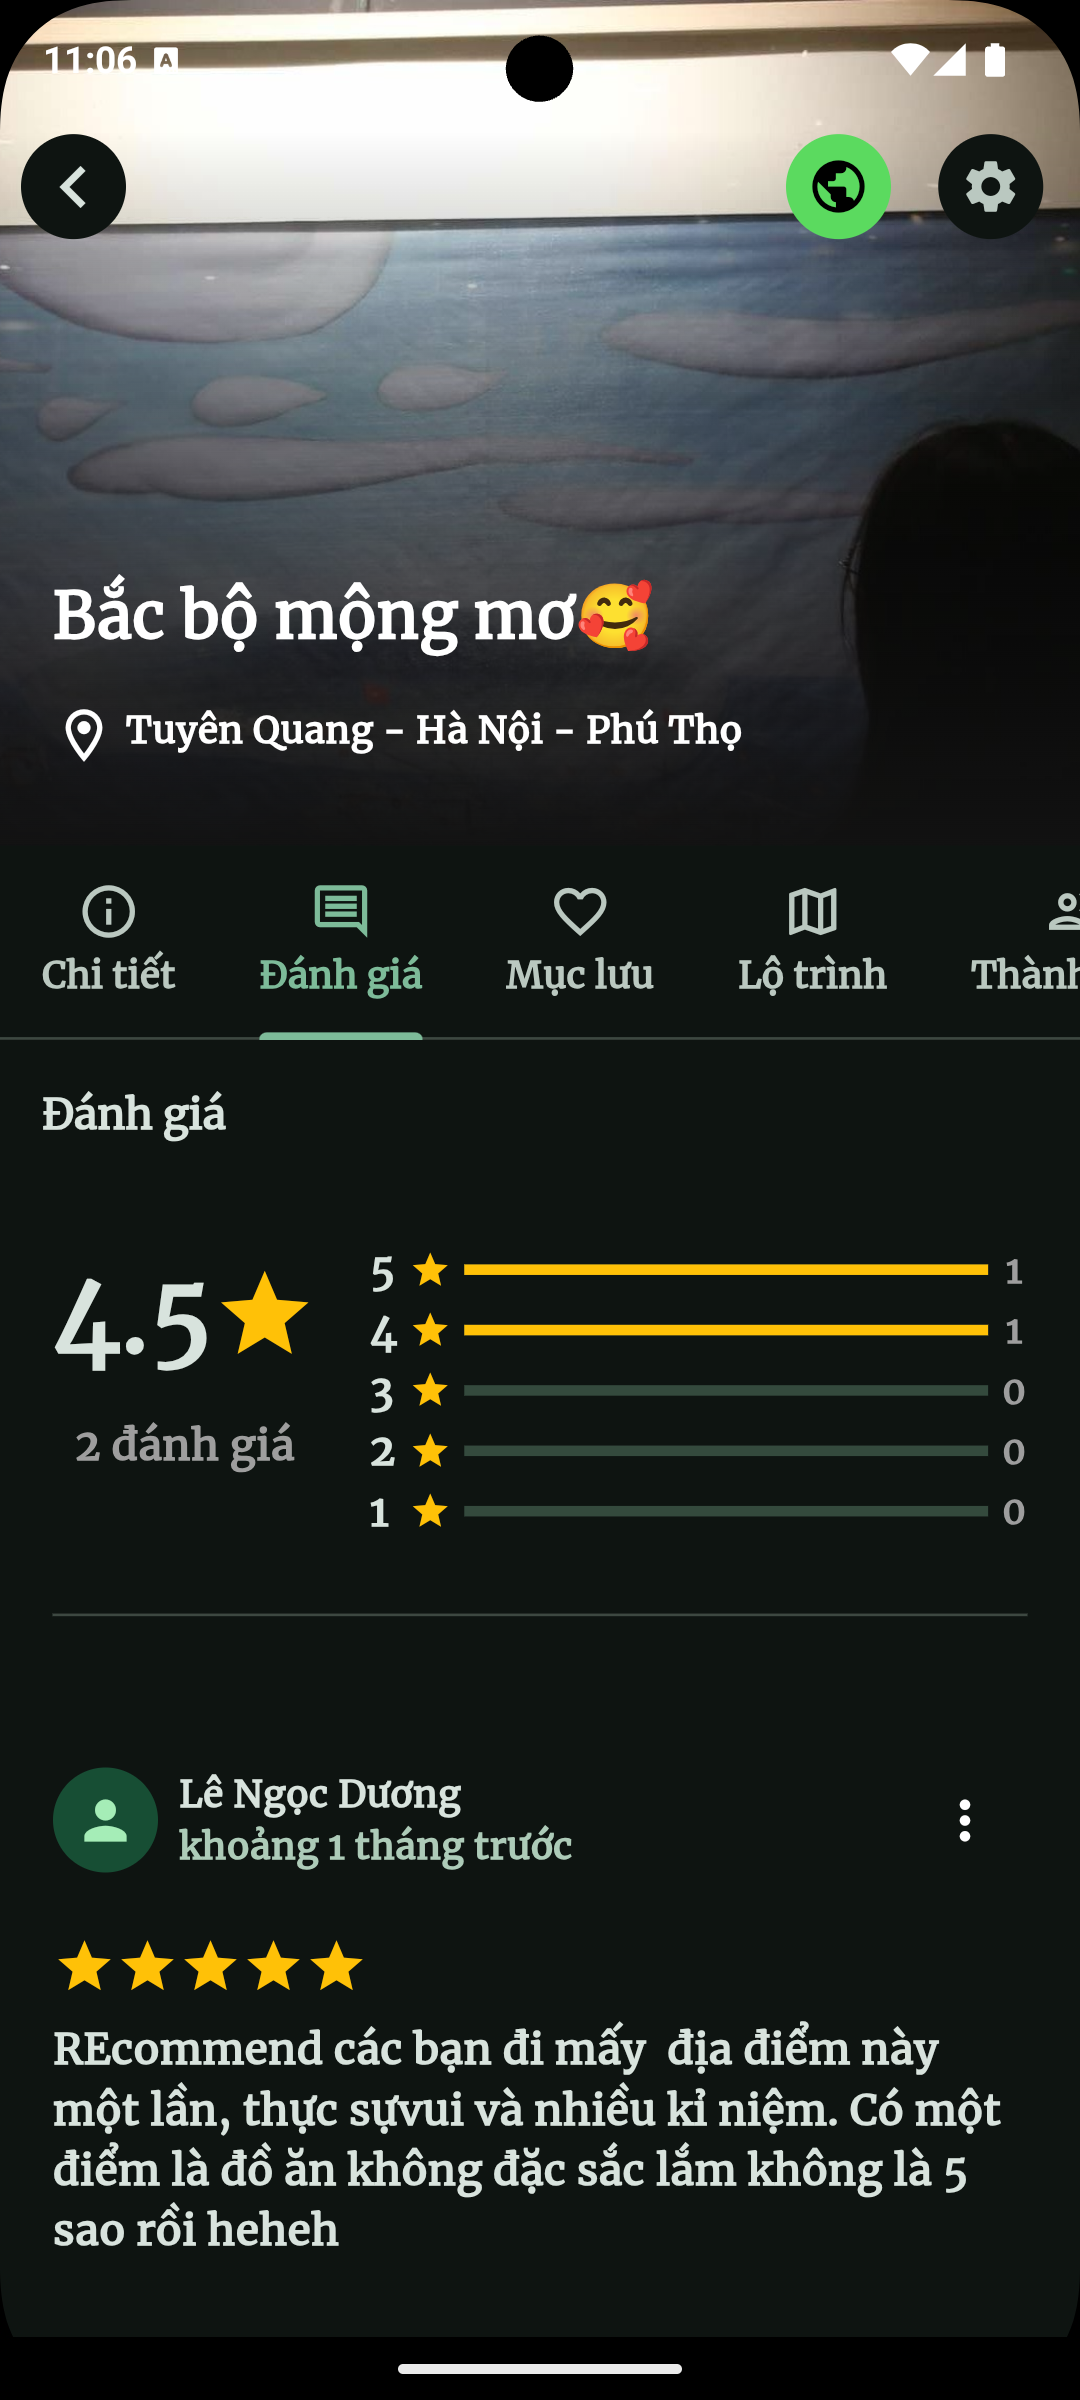
\includegraphics[width=1\linewidth]{figures/c4/system_func/trip_rating.png}
        \caption{Đánh giá chuyến đi}
        \label{fig:func_trip_rating}
    \end{subfigure}
    \hfill
    \begin{subfigure}{0.326\textwidth}
        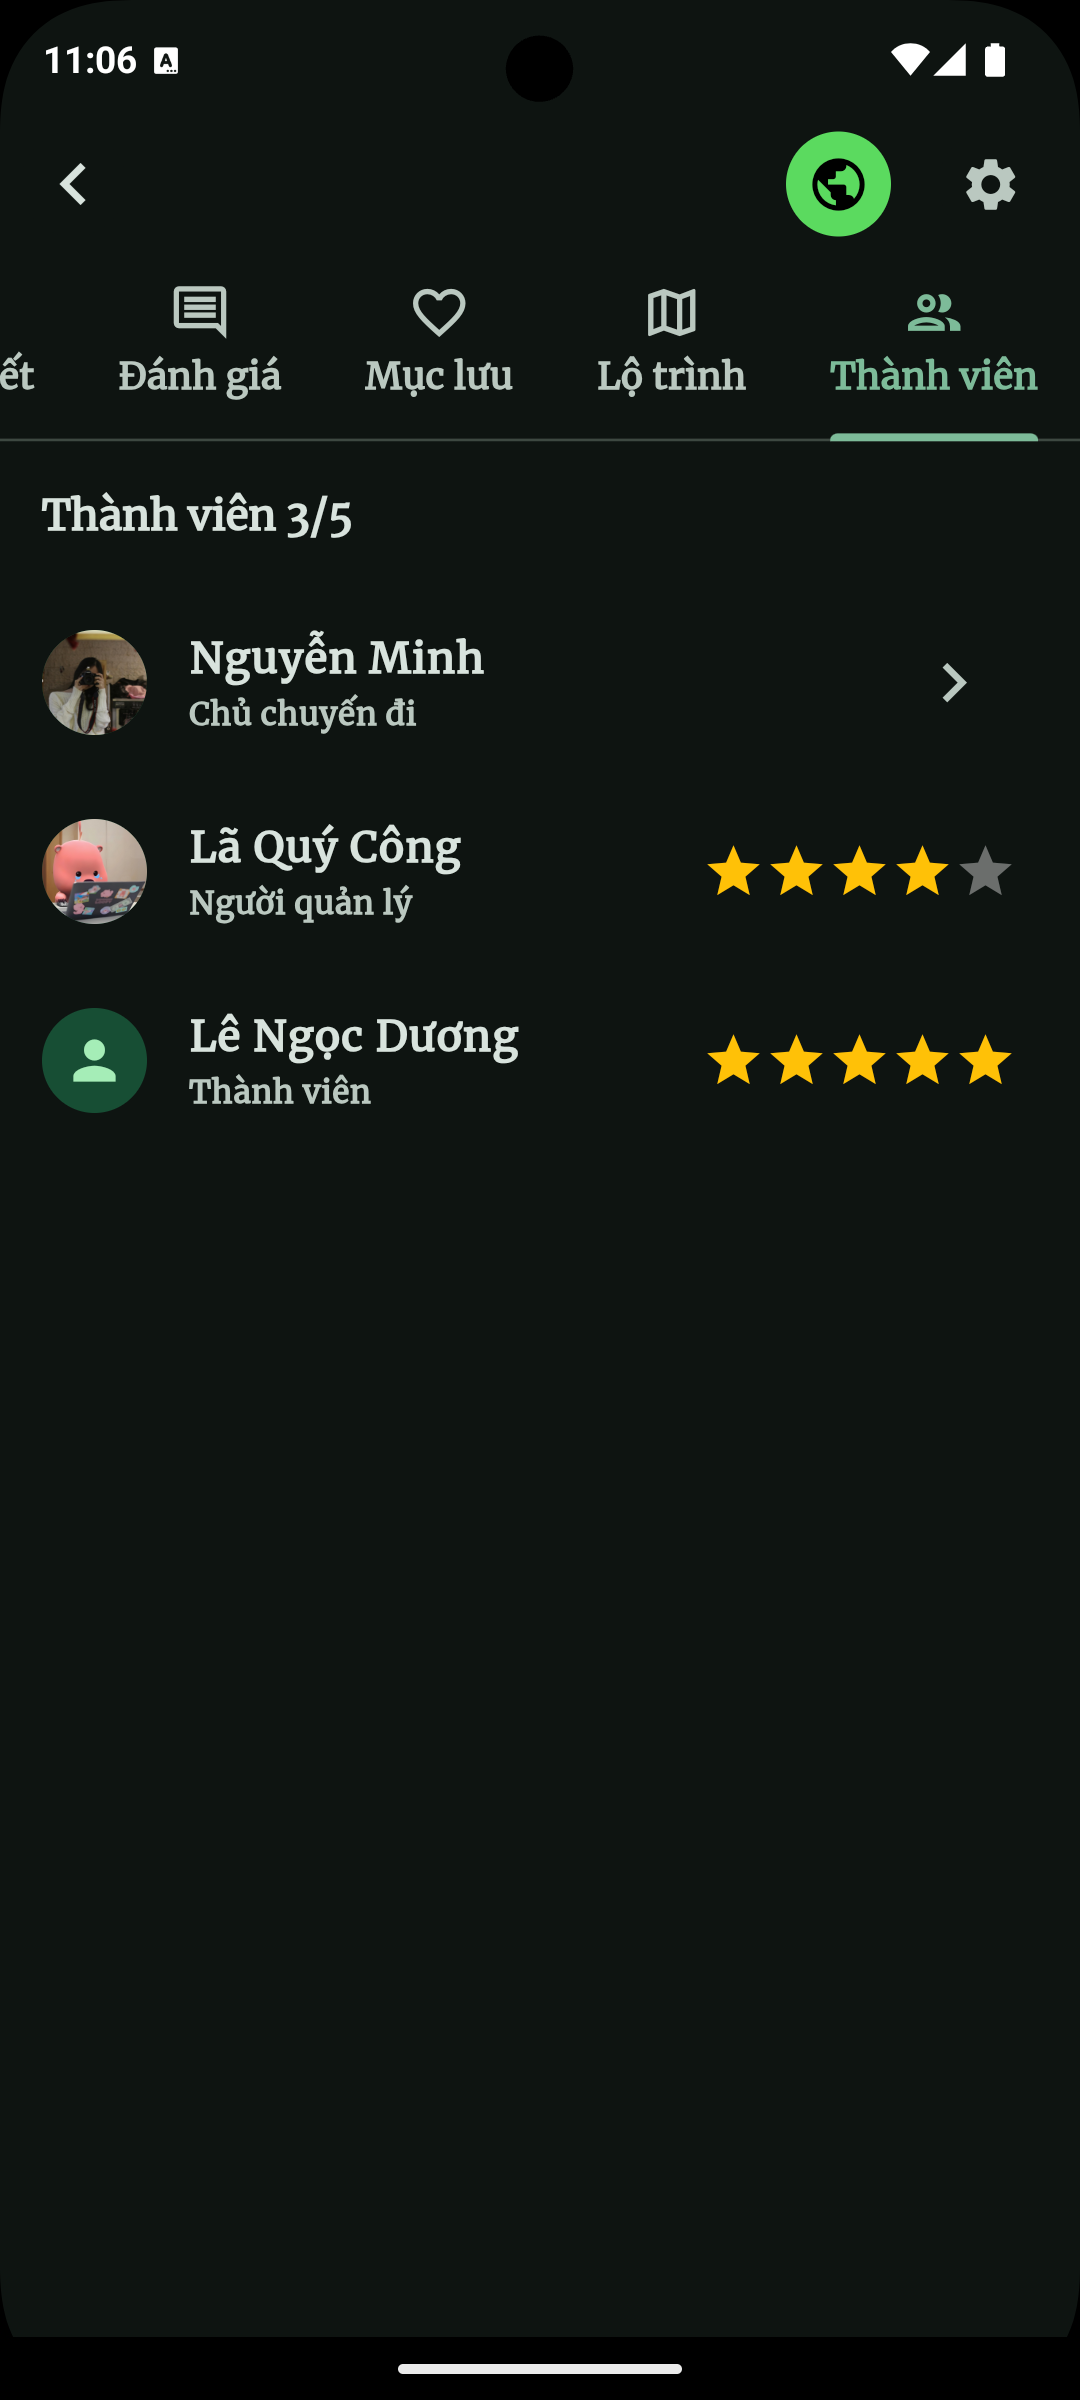
\includegraphics[width=1\linewidth]{figures/c4/system_func/rating_member.png}
        \caption{Đánh giá thành viên}
        \label{fig:func_member_rating}
    \end{subfigure}
    \caption{Các chức năng trong và sau chuyến đi.}
    \label{fig:trip-management-3}
\end{figure}

\subsection{Tin nhắn và Tổng hợp Lịch trình}
\noindent Người dùng có thể nhắn tin với các thành viên trong cùng chuyến đi hoặc nhắn tin riêng với người dùng khác. Hệ thống cung cấp các tính năng nhắn tin cơ bản như gửi/gỡ tin nhắn, hiển thị trạng thái ``đã xem", và phản hồi tin nhắn (reaction) trong thời gian thực (Hình~\ref{fig:messaging-1}), với giao diện nhắn tin chính (Hình~\ref{fig:func_messages}), danh sách các cuộc hội thoại (Hình~\ref{fig:func_inbox}), và ví dụ về phản hồi tin nhắn (Hình~\ref{fig:func_react}).

\begin{figure}[H]
    \centering
    \begin{subfigure}{0.326\textwidth}
        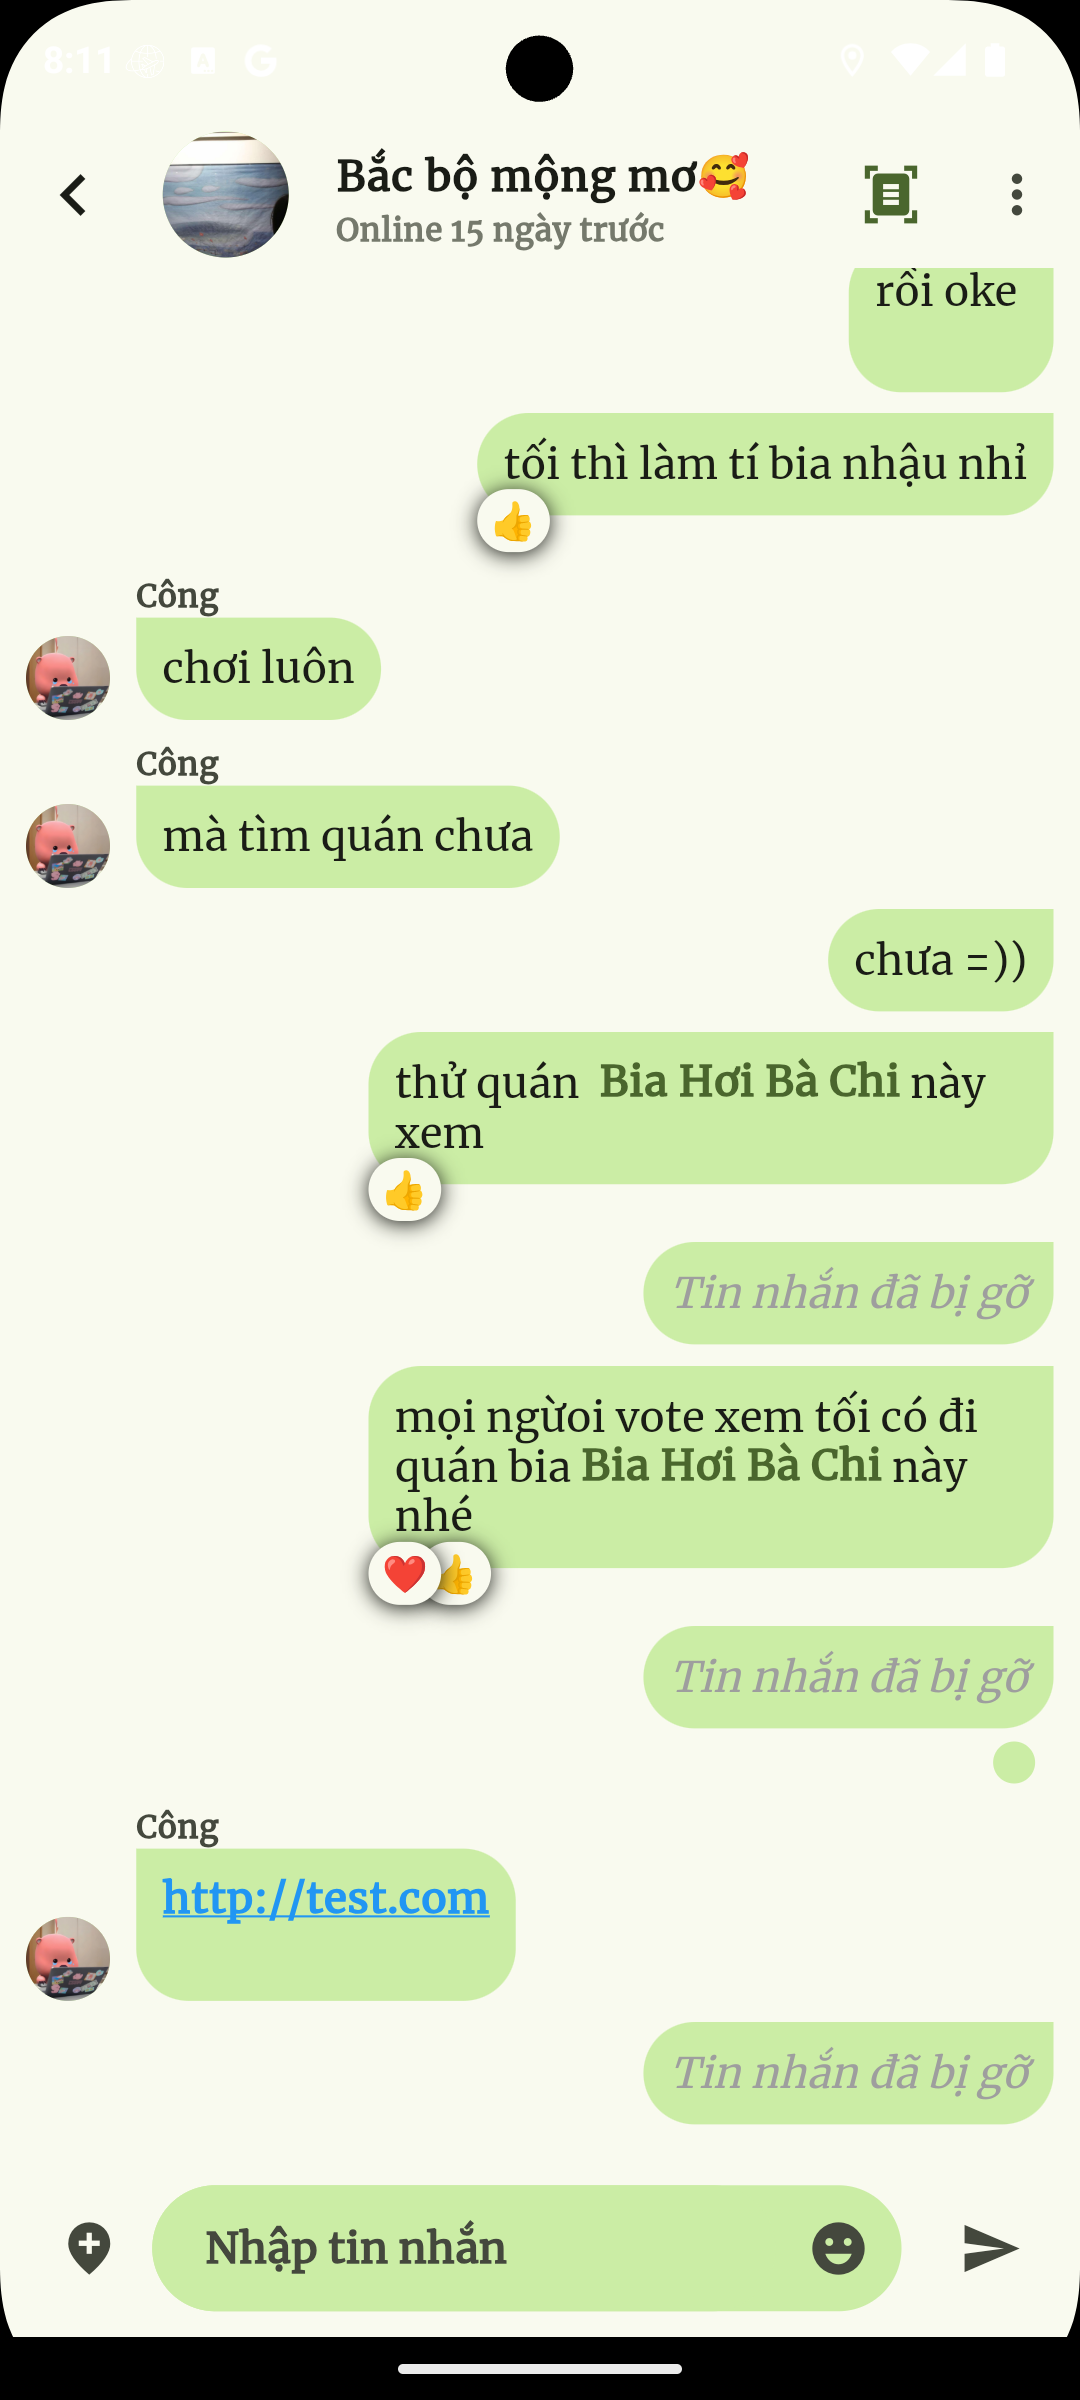
\includegraphics[width=1\linewidth]{figures/c4/system_func/inbox.png}
        \caption{Giao diện nhắn tin}
        \label{fig:func_messages}
    \end{subfigure}
    \hfill
    \begin{subfigure}{0.326\textwidth}
        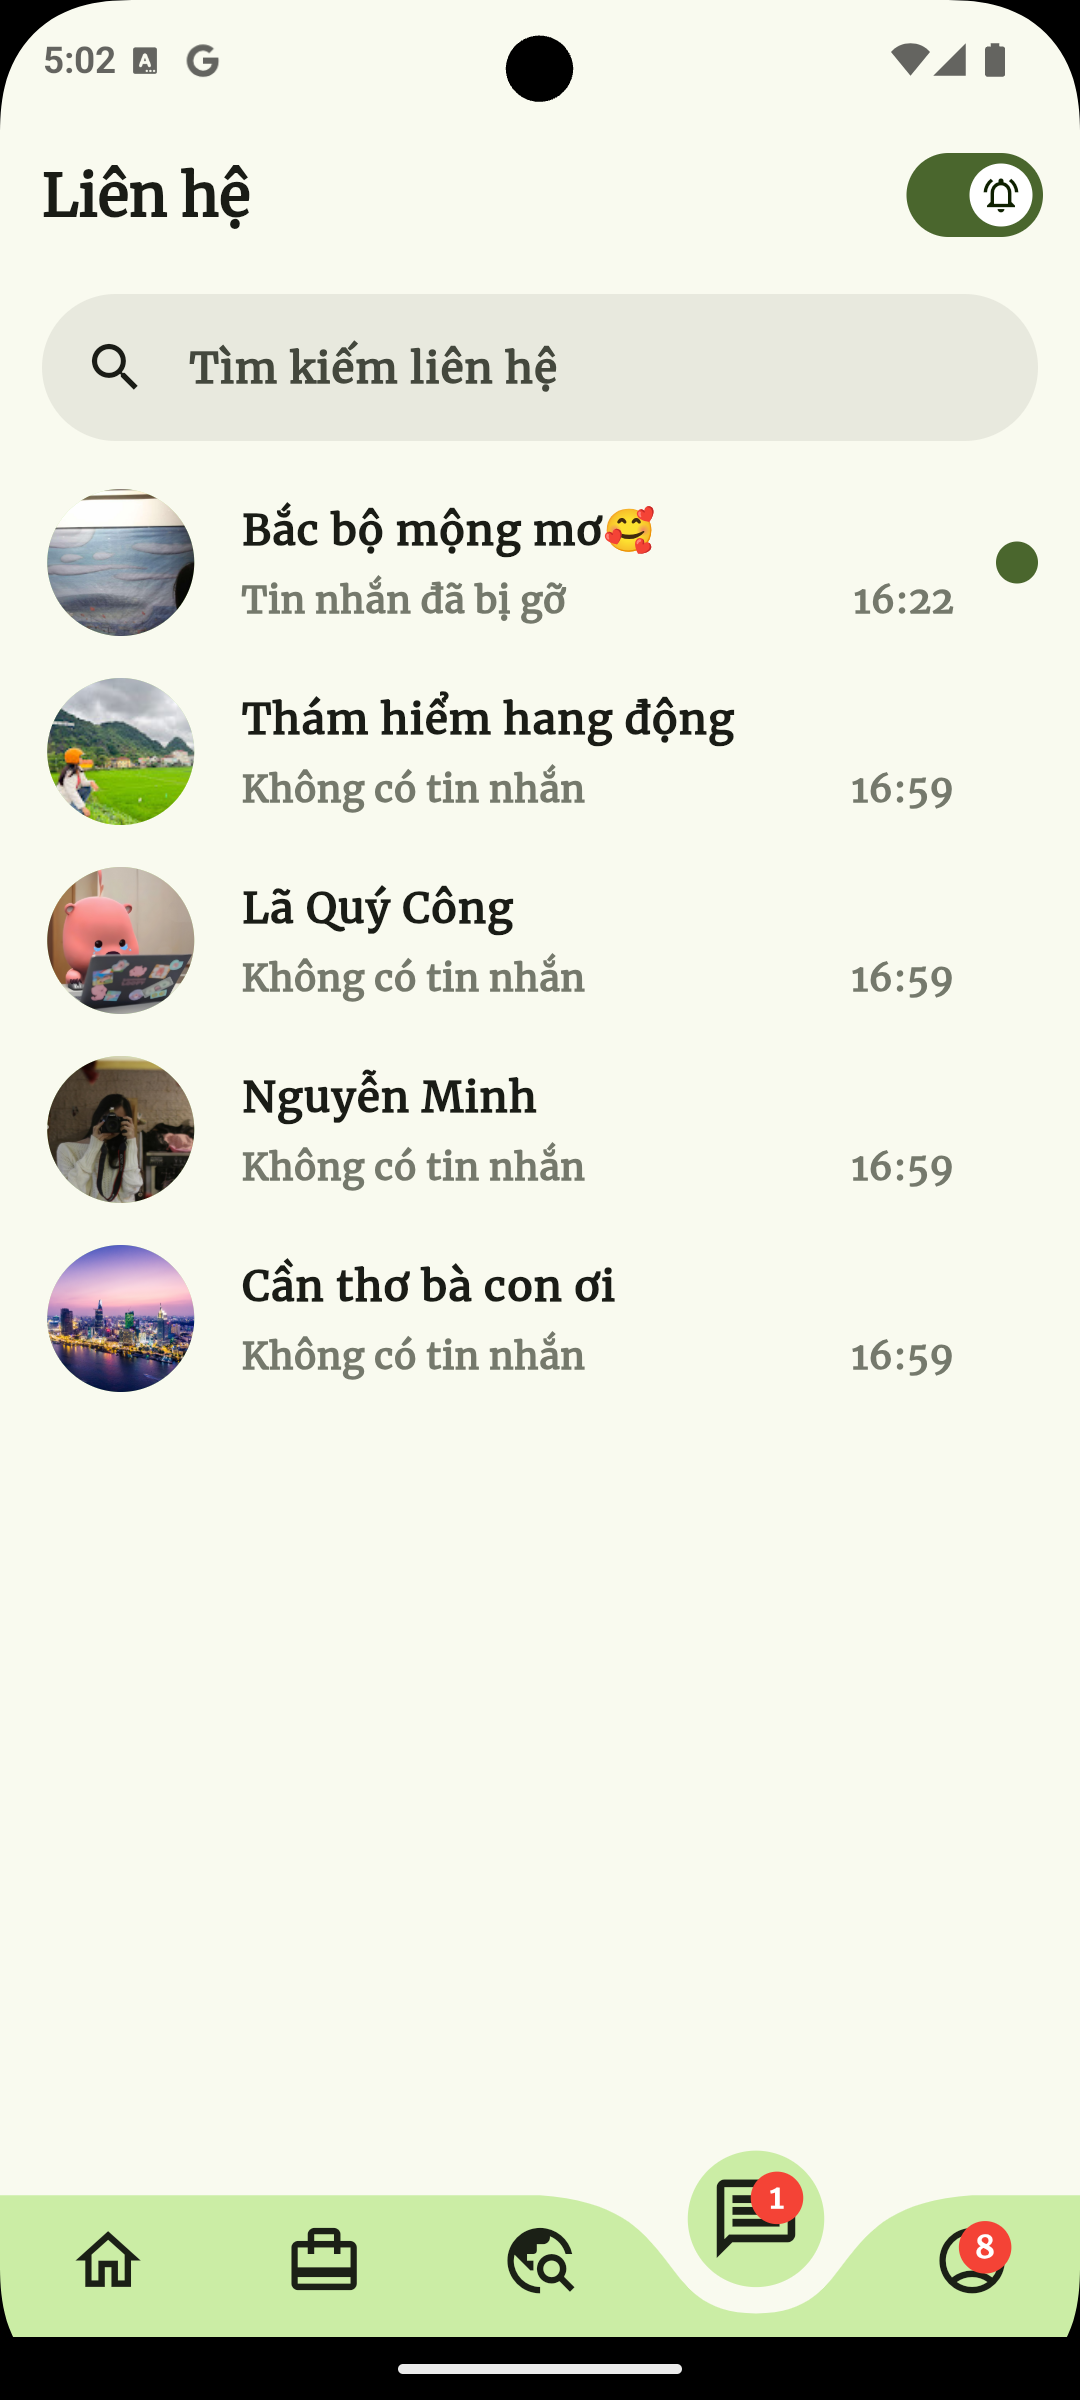
\includegraphics[width=1\linewidth]{figures/c4/system_func/messages.png}
        \caption{Danh sách hội thoại}
        \label{fig:func_inbox}
    \end{subfigure}
    \hfill
    \begin{subfigure}{0.326\textwidth}
        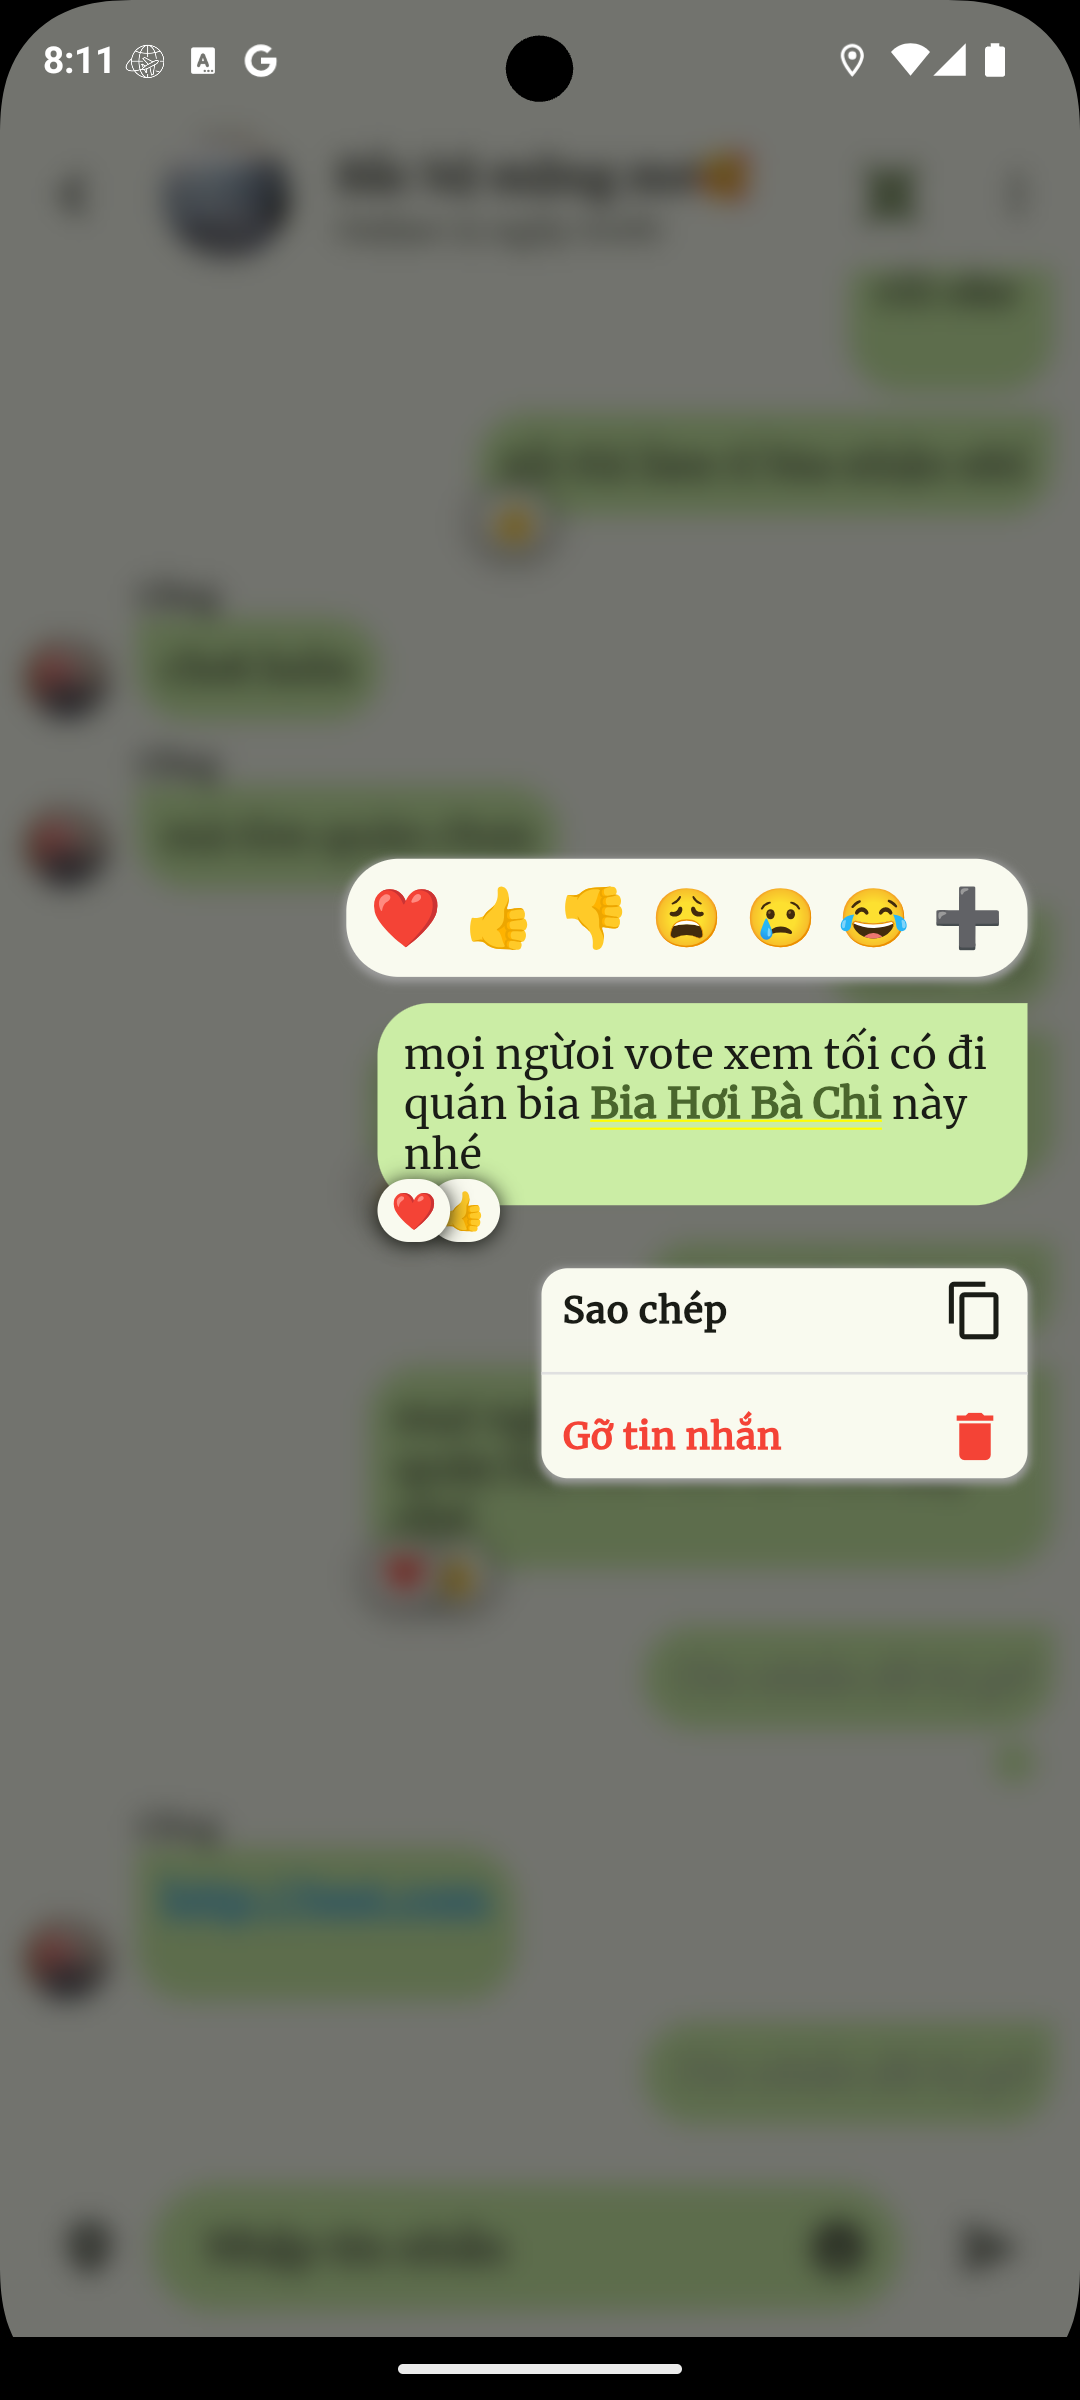
\includegraphics[width=1\linewidth]{figures/c4/system_func/react.png}
        \caption{React tin nhắn/Vote}
        \label{fig:func_react}
    \end{subfigure}
    \caption{Giao diện nhắn tin cơ bản.}
    \label{fig:messaging-1}
\end{figure}

\noindent \noindent Điểm đặc biệt của VieVu là các tính năng AI tích hợp trong giao diện nhắn tin (Hình~\ref{fig:messaging-2}). Người dùng có thể gắn thẻ (tag) địa điểm trực tiếp vào tin nhắn để thảo luận (Hình~\ref{fig:func_tag_loc}). Hệ thống tự động phân tích nội dung hội thoại và cho phép người dùng xem bản tóm tắt các ý chính (Recap - Hình~\ref{fig:func_recap}). Quan trọng nhất, người dùng có thể yêu cầu hệ thống tổng hợp toàn bộ cuộc thảo luận thành một bản nháp lịch trình chi tiết (Hình~\ref{fig:func_summary_result}), bản nháp này sau đó có thể được chuyển thành lịch trình chính thức của chuyến đi.

\begin{figure}[H]
    \centering
    \begin{subfigure}{0.326\textwidth}
        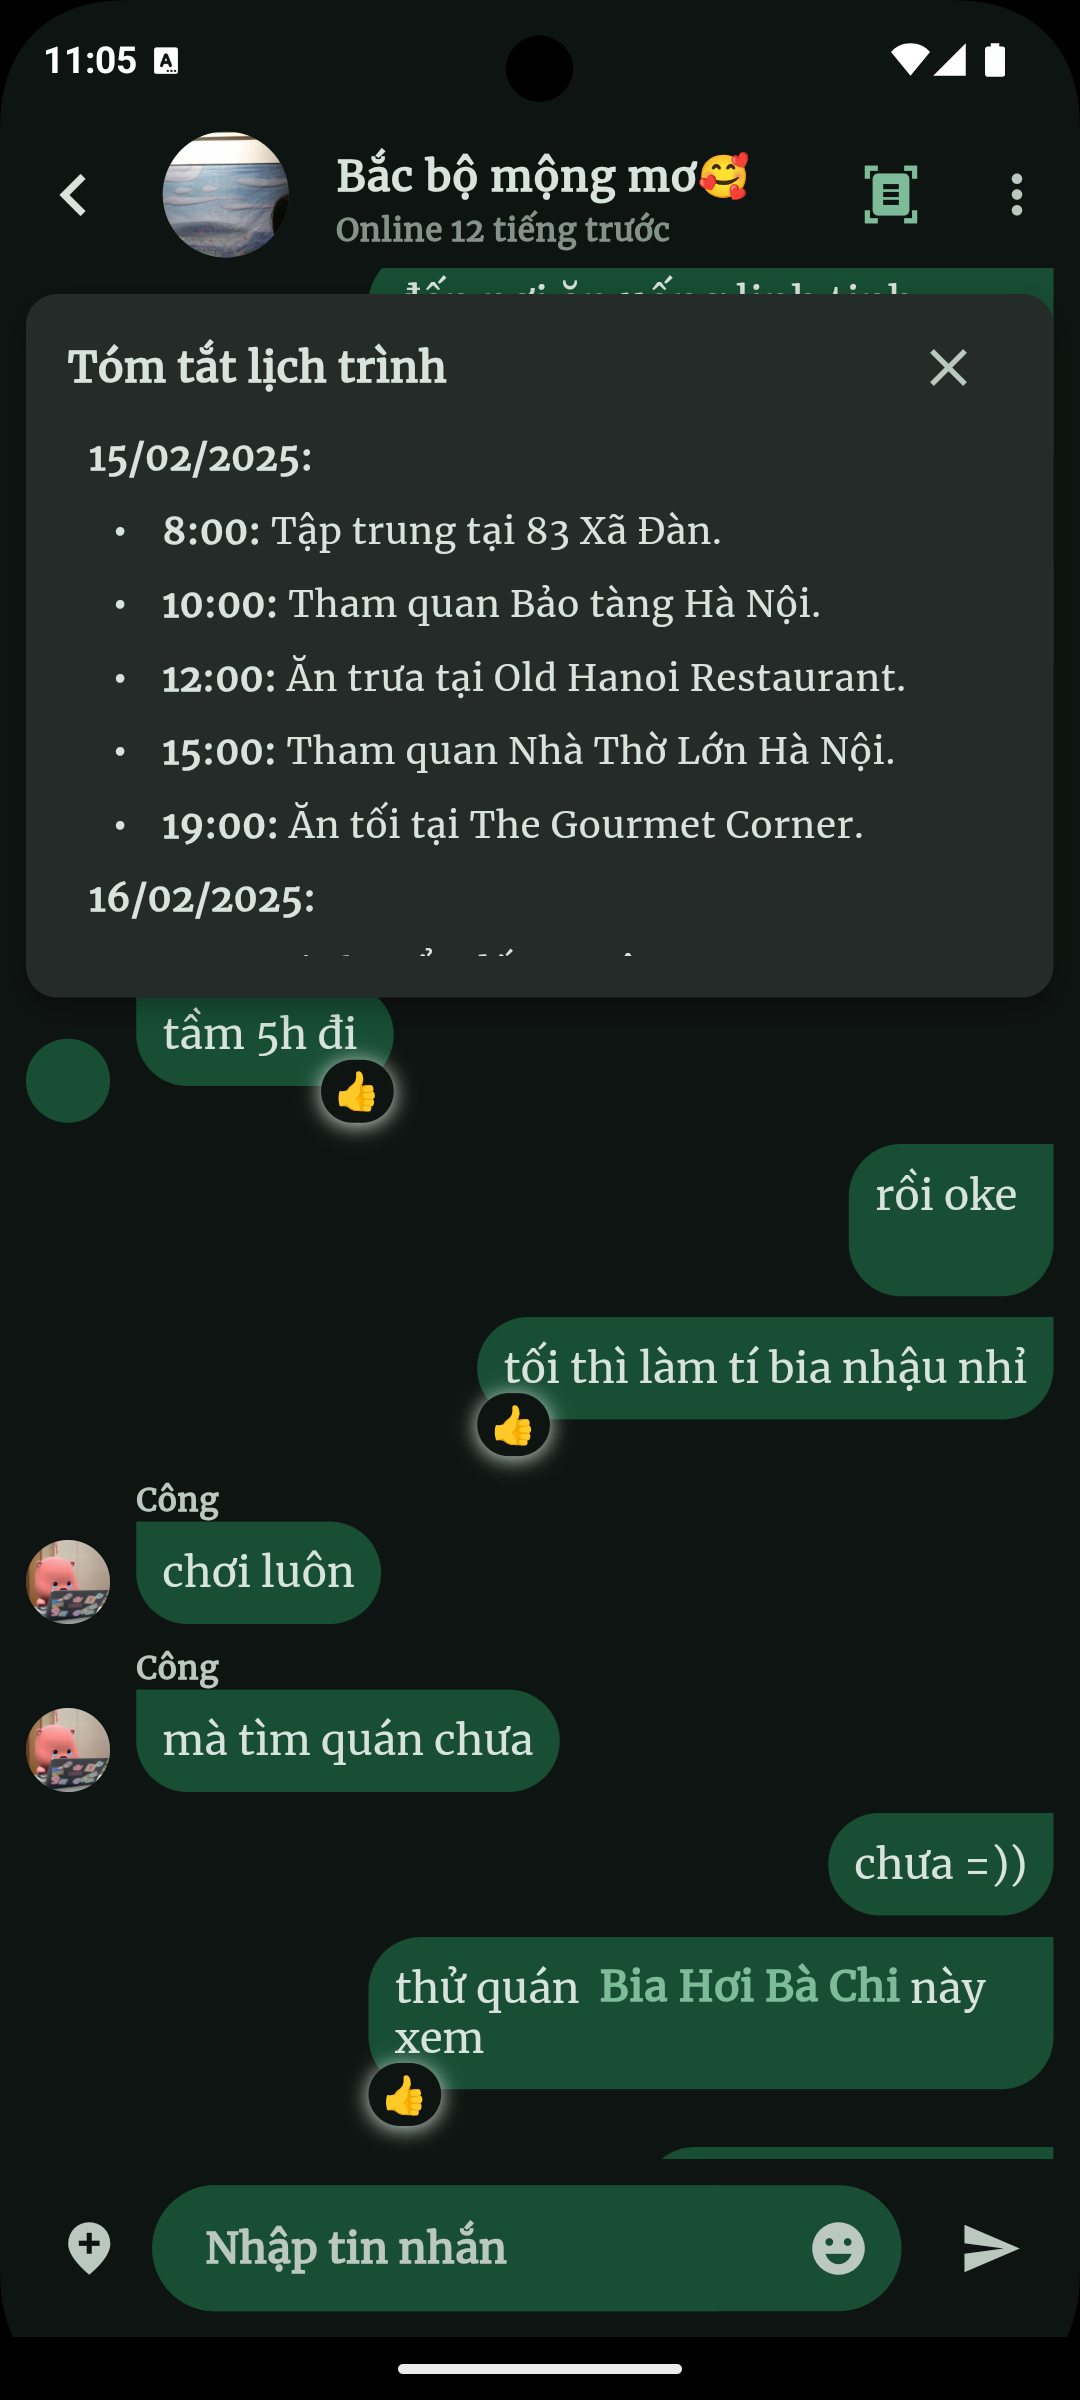
\includegraphics[width=1\linewidth]{figures/c4/system_func/recap.png}
        \caption{Xem tóm tắt (Recap)}
        \label{fig:func_recap}
    \end{subfigure}
    \hfill
    \begin{subfigure}{0.326\textwidth}
        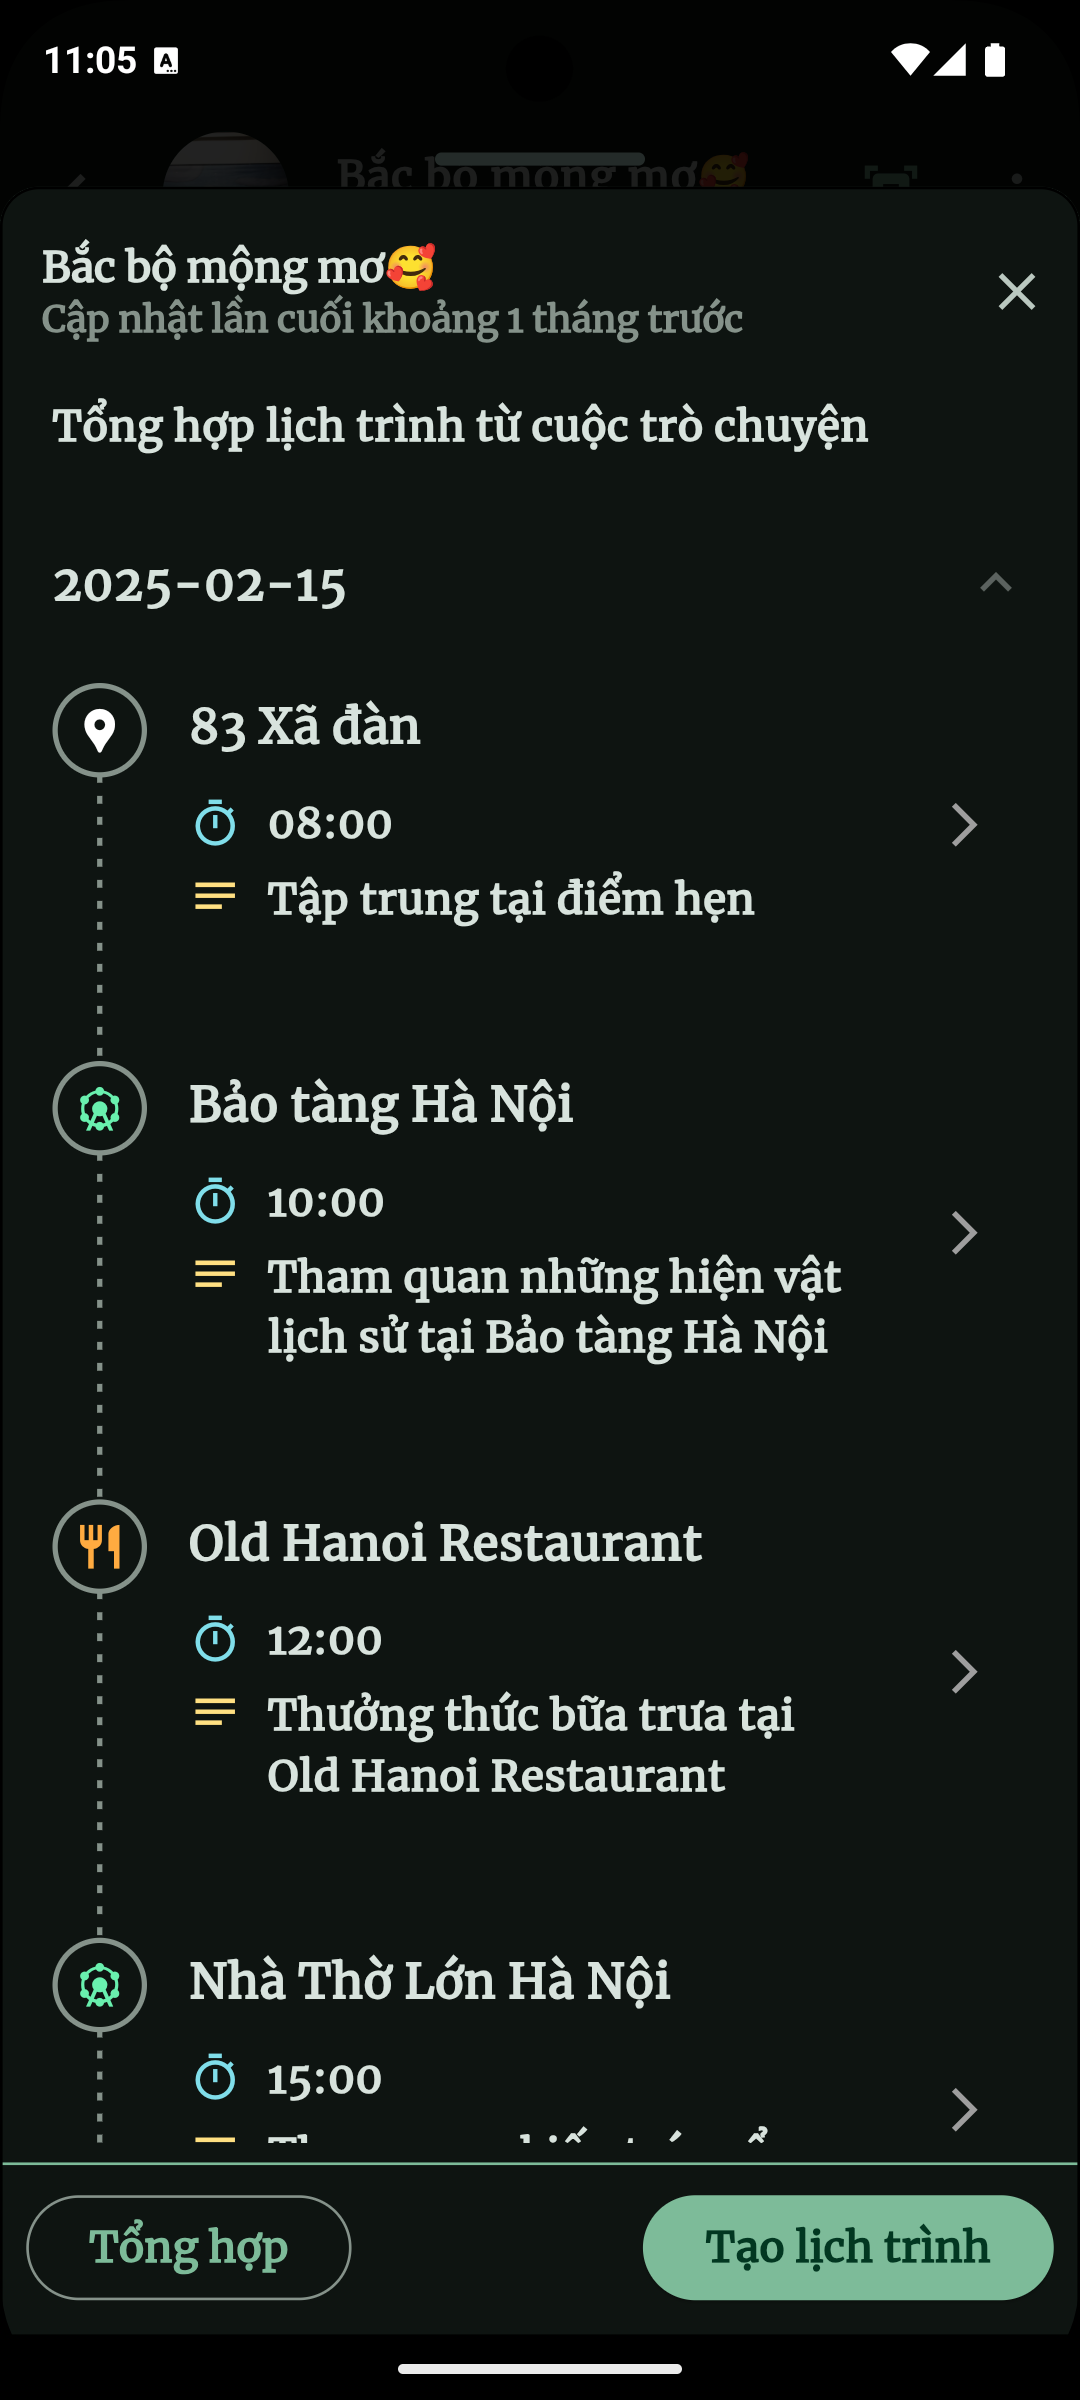
\includegraphics[width=1\linewidth]{figures/c4/system_func/summa.png}
        \caption{Lịch trình tổng hợp}
        \label{fig:func_summary_result}
    \end{subfigure}
    \hfill
    \begin{subfigure}{0.326\textwidth}
        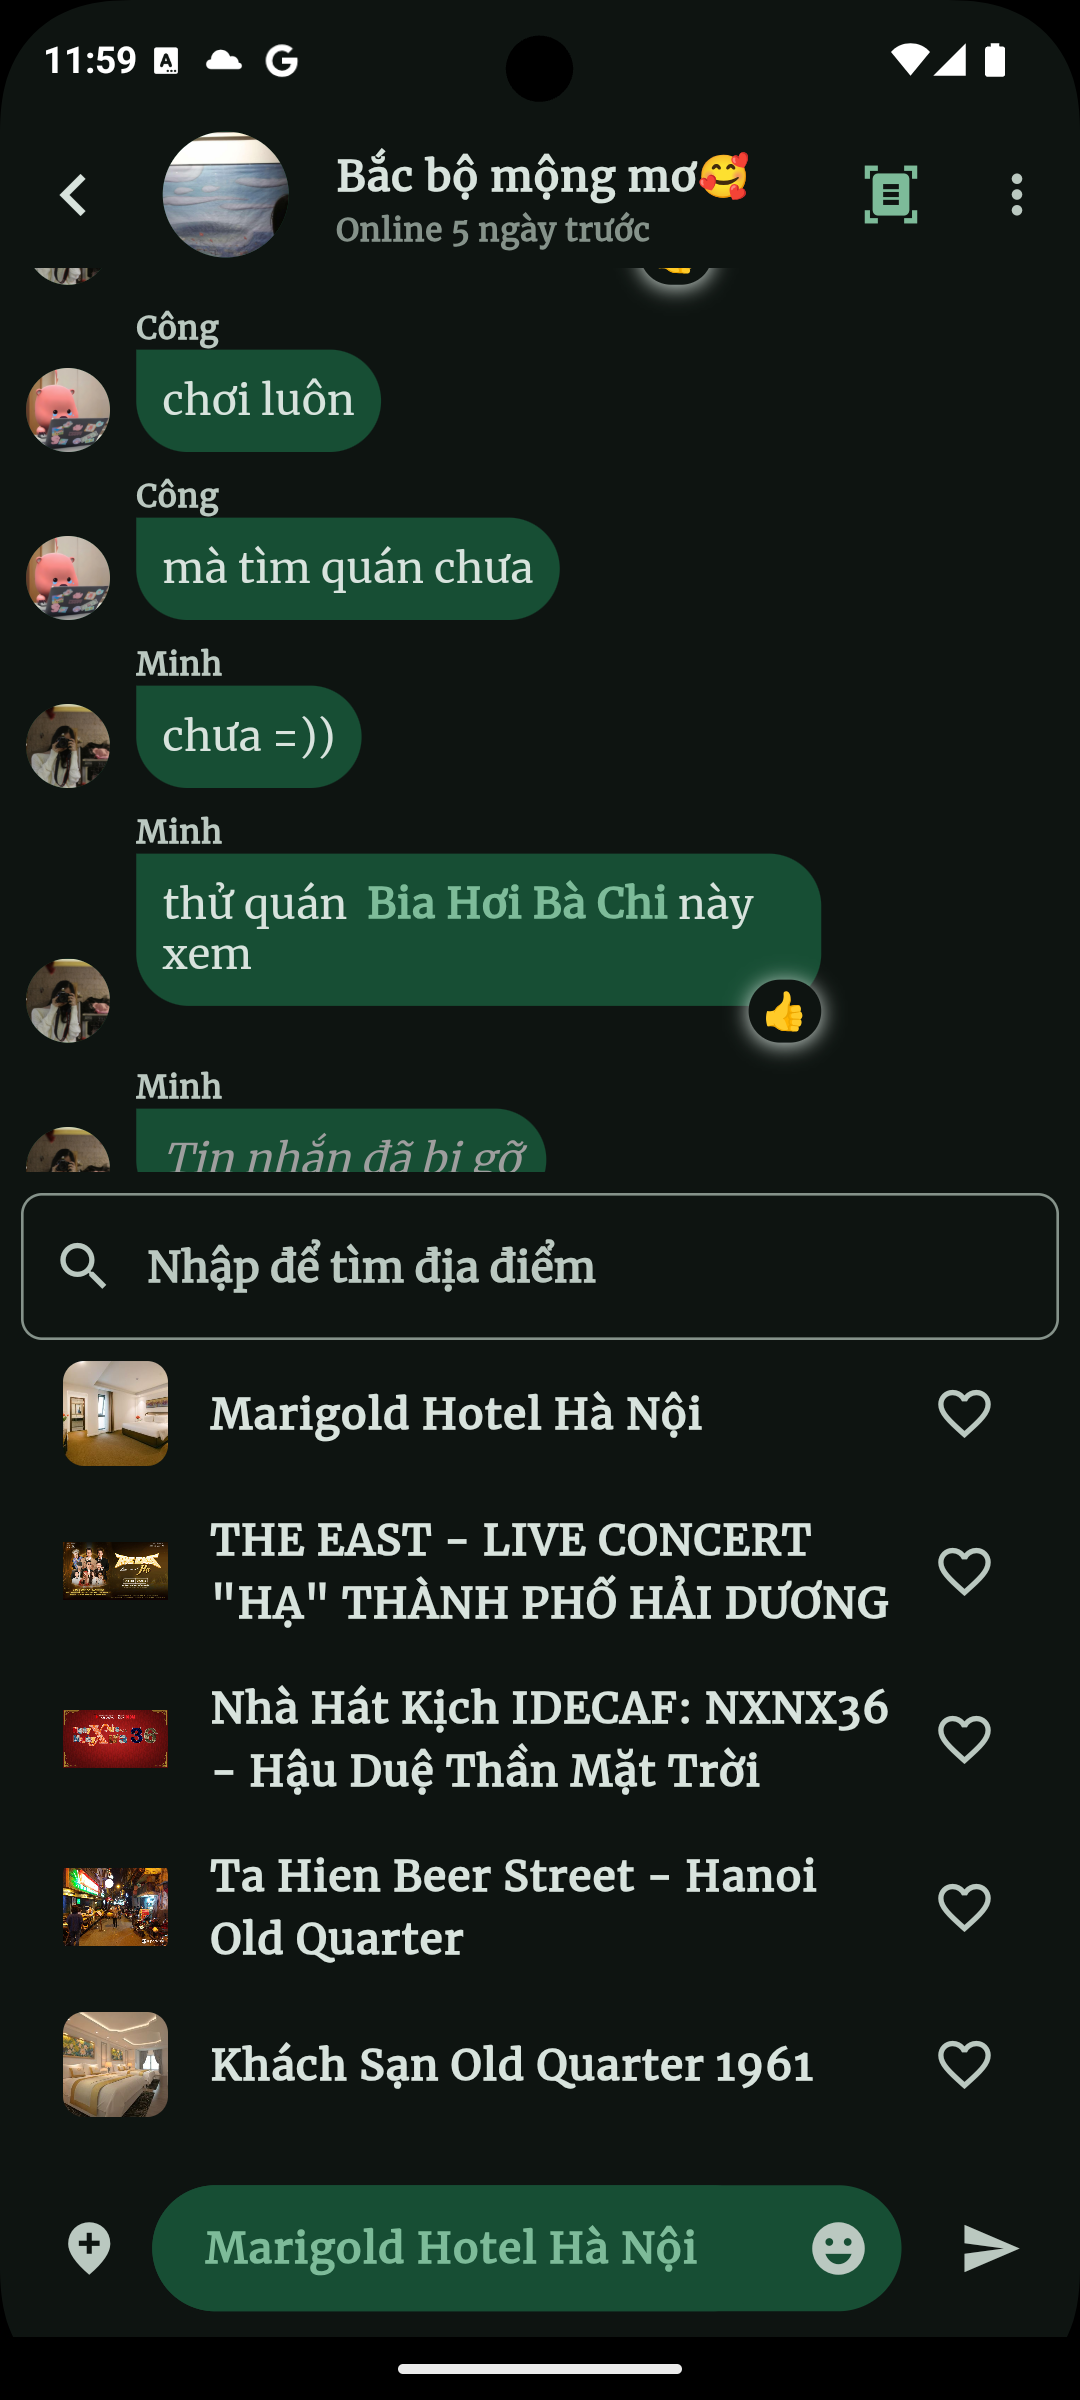
\includegraphics[width=1\linewidth]{figures/c4/system_func/tag_loc.png}
        \caption{Gắn thẻ địa điểm}
        \label{fig:func_tag_loc}
    \end{subfigure}
    \caption{Các tính năng AI trong nhắn tin.}
    \label{fig:messaging-2}
\end{figure}

\subsection{Các chức năng khác}
\noindent Ngoài các chức năng chính đã nêu, hệ thống VieVu còn cung cấp một số tiện ích khác nhằm nâng cao trải nghiệm người dùng (Hình~\ref{fig:other-functions}). Chức năng gợi ý địa điểm (Hình~\ref{fig:func_recommend}) đề xuất các lựa chọn phù hợp dựa trên sở thích và hành vi người dùng. Hệ thống thông báo đẩy (Hình~\ref{fig:func_noti}) giúp người dùng cập nhật các sự kiện quan trọng. Người dùng cũng có thể tùy chỉnh giao diện sáng/tối của ứng dụng (Hình~\ref{fig:func_theme}).

\begin{figure}[H]
    \centering
    \begin{subfigure}{0.326\textwidth}
        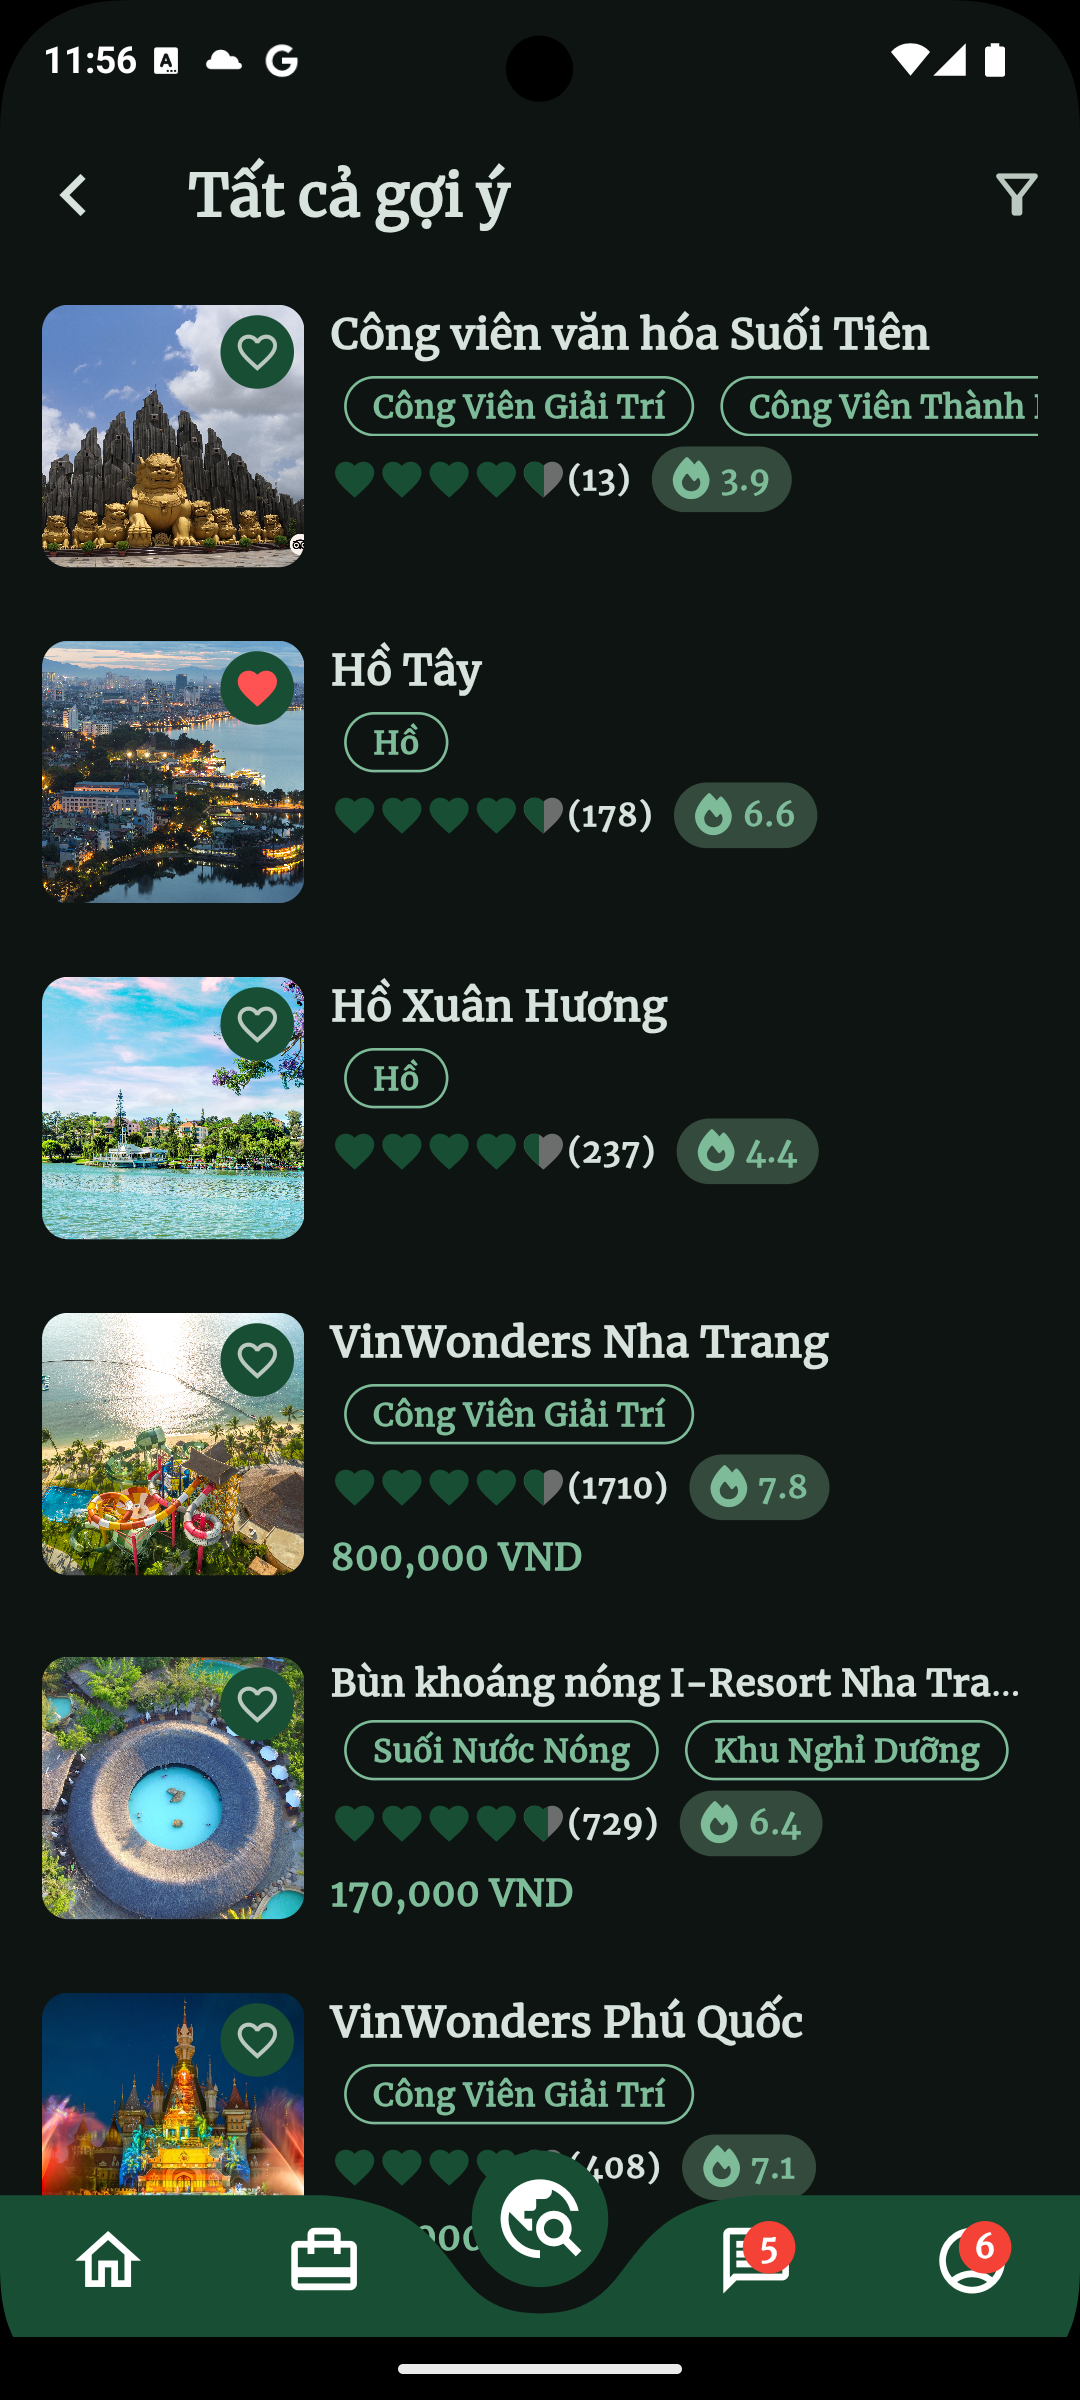
\includegraphics[width=1\linewidth]{figures/c4/system_func/recommend.png}
        \caption{Gợi ý địa điểm}
        \label{fig:func_recommend}
    \end{subfigure}
    \hfill
    \begin{subfigure}{0.326\textwidth}
        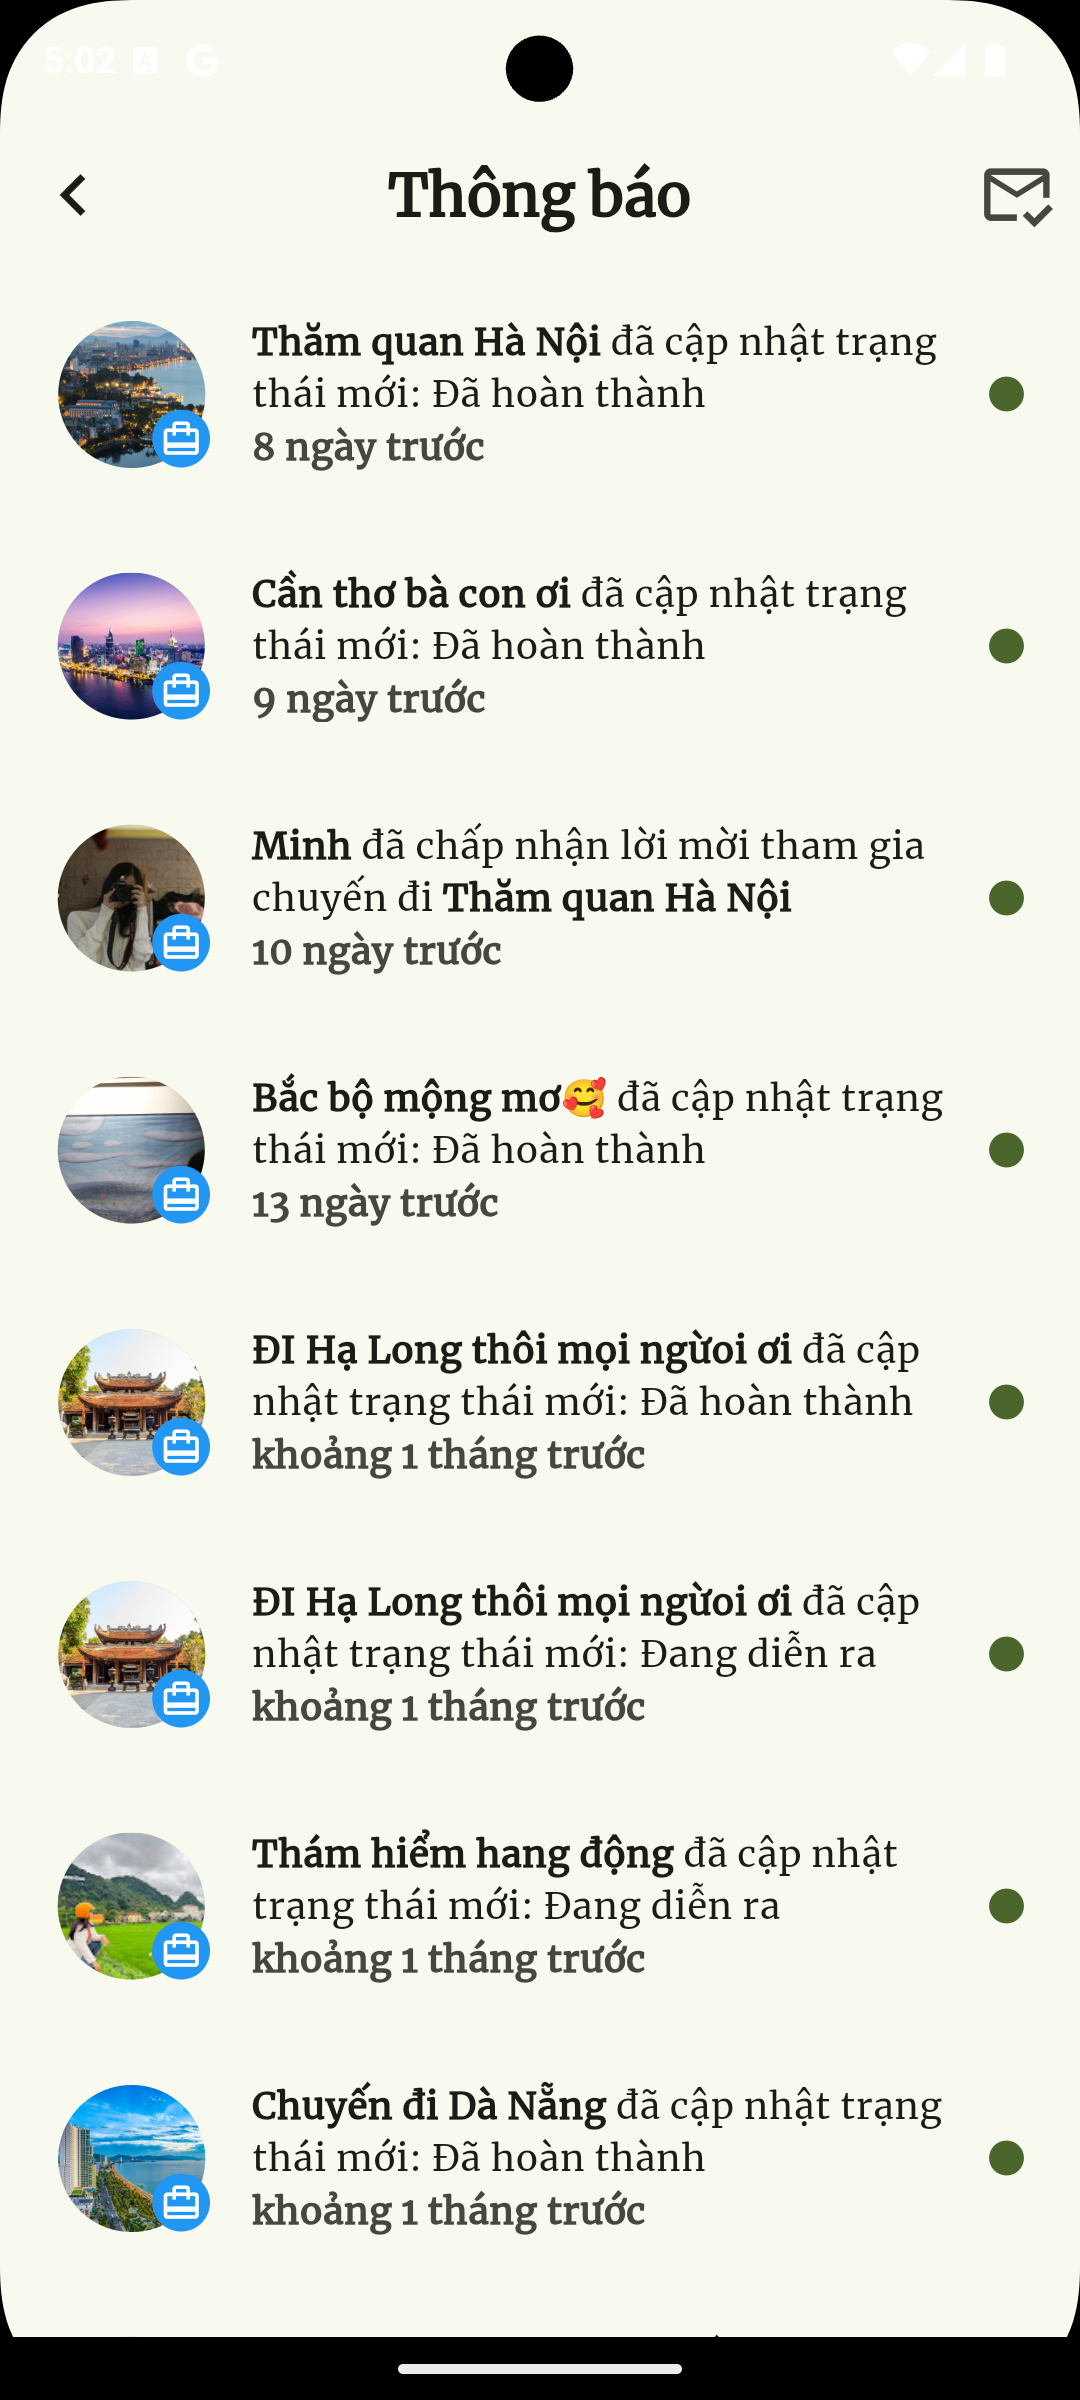
\includegraphics[width=1\linewidth]{figures/c4/system_func/noti.png}
        \caption{Thông báo}
        \label{fig:func_noti}
    \end{subfigure}
    \hfill
    \begin{subfigure}{0.326\textwidth}
        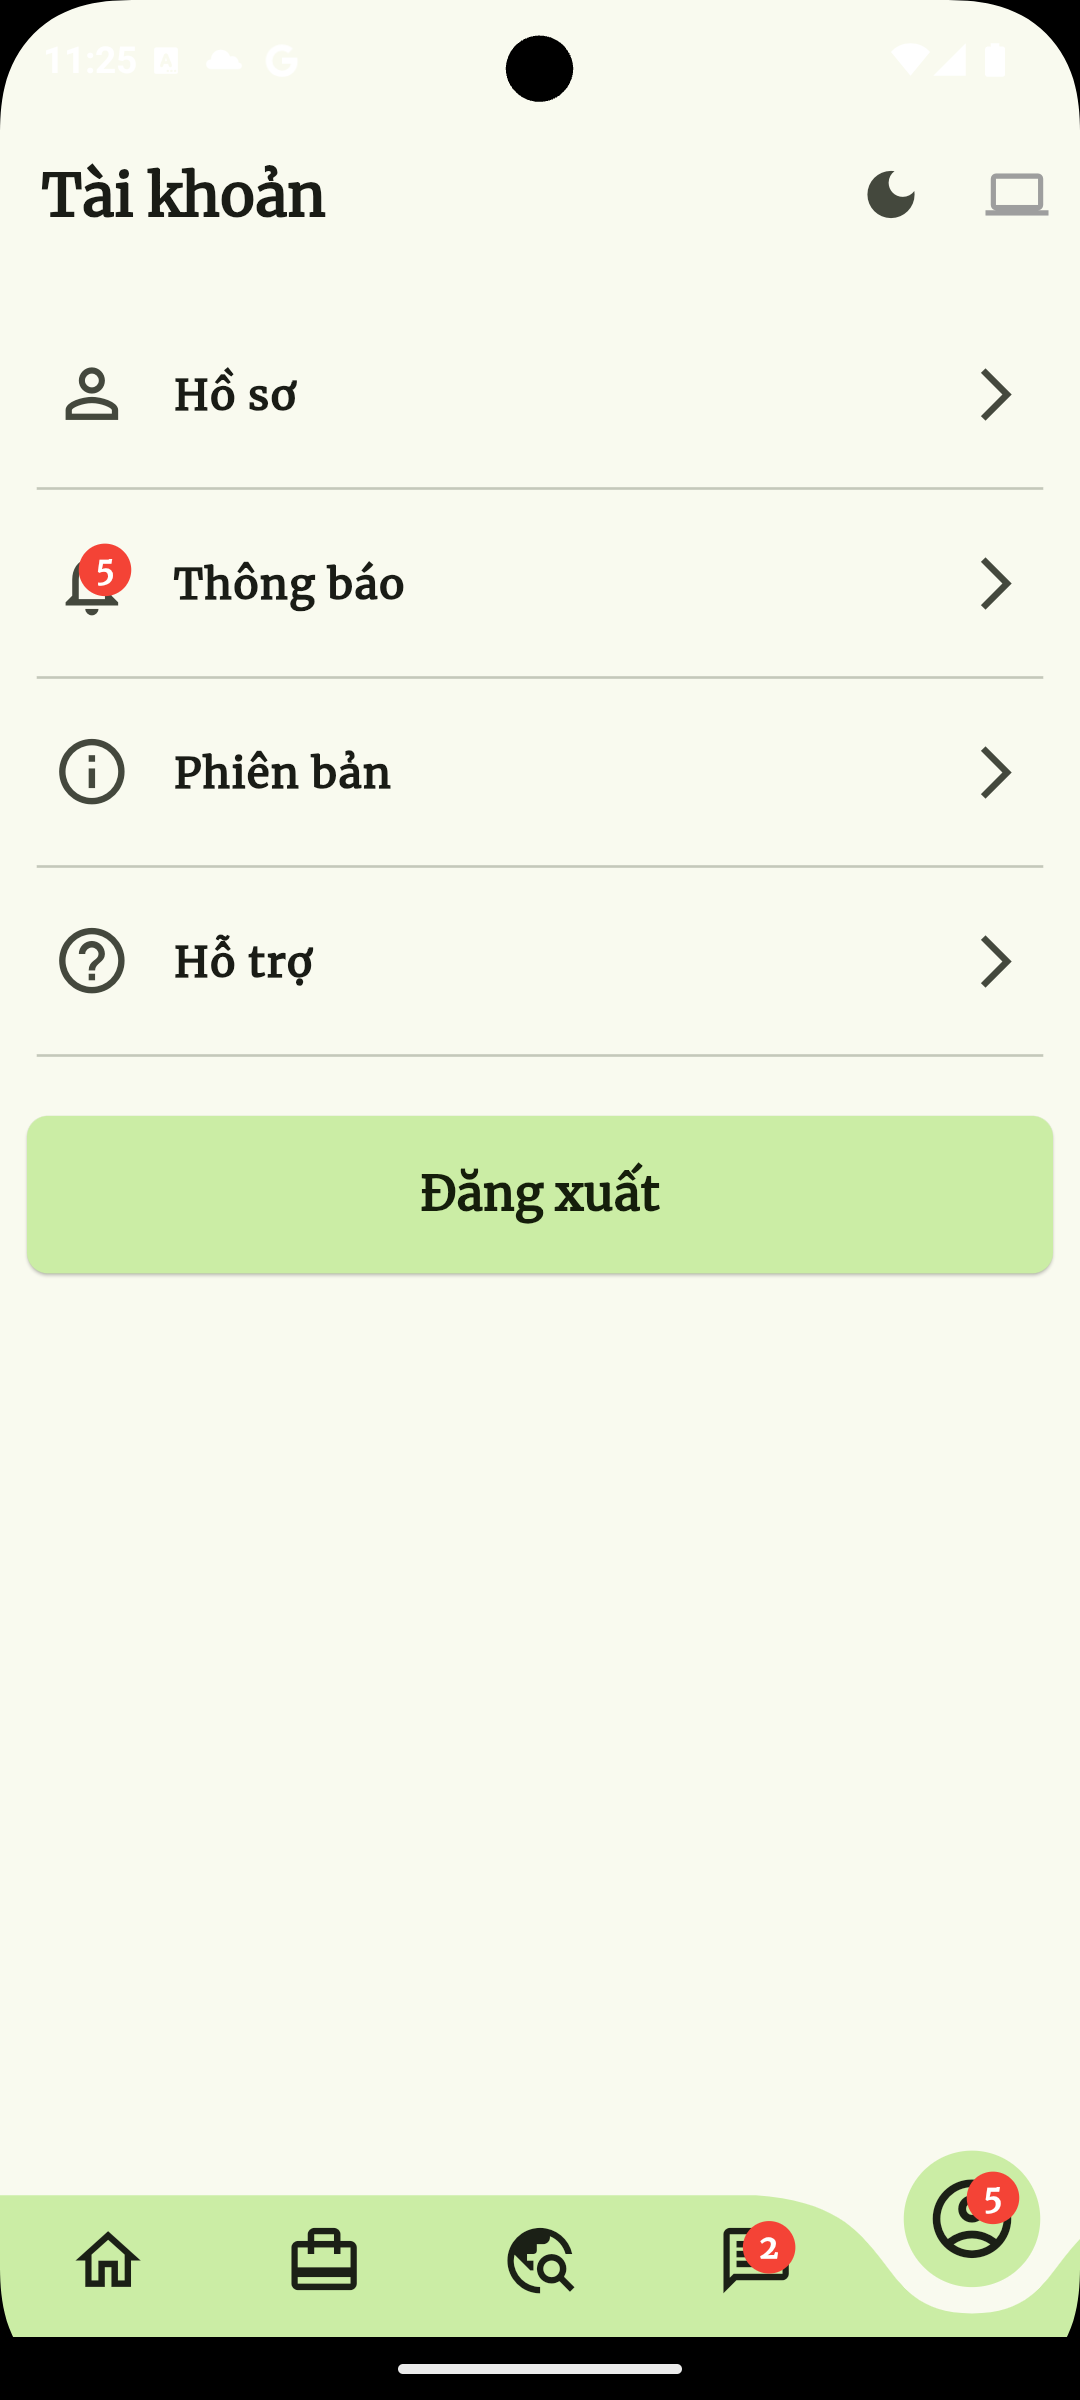
\includegraphics[width=1\linewidth]{figures/c4/system_func/theme.png}
        \caption{chọn theme màu}
        \label{fig:func_theme}
    \end{subfigure}
    \caption{Một số chức năng khác.}
    \label{fig:other-functions}
\end{figure}